\ifx \notincludehead\undefined
	\newcommand*{\No}{\textnumero}
	\documentclass[russian, utf8, 12pt, pointsubsection,floatsubsection]{eskdtext}
	\usepackage[russian]{babel}

	\ifx\pdfoutput\undefined  
		\def\pdfoutput{0}
	\fi

	\ifnum\pdfoutput=0 
		\sloppy
		%	\usepackage[dvips]{graphicx}       % загрузка графики под dvi  
		\textheight=250mm                  % для DVI высота печатного текста
		\textwidth=165mm                   % ширина печатного текста
	\else
		%	\usepackage[pdftex]{graphicx}      % загрузка графики под pdf
		\usepackage{cmap}                  % чтоб работал поиск по PDF 
		% гиперссылки в PDF
		\usepackage[unicode, pdftex, colorlinks, linkcolor=blue]{hyperref} 
		\pdfcompresslevel=9                % сжимаем PDF 
		%	\textheight=240mm                  % для PDF высота печатного текста
		%	\textwidth=165mm                   % ширина печатного текста
	\fi 

	\usepackage{eskdchngsheet}
	\usepackage[T2A]{fontenc}
	%\usepackage[cp1251]{inputenc}
	\usepackage{amstext}
	\usepackage{amsmath}
	\usepackage{listings}
	\usepackage{rotating}
	\usepackage{pmasc}
	\usepackage{todonotes}
	
	
	\usepackage{datetime}
	
% 	\usepackage{CJK} % ПОДДЕРЖКА КИТАЙСКОГО ЯЗЫКА  xeCJK
    

	\usepackage{placeins}    % пакет позволяет вставлять плавающие объекты (рисунки) в том месте, 
                         % где это необходимо. Для вывода рисунка после него встаить команду \FloatBarrier

	\usepackage{array}
	\usepackage{longtable}   % подключение длинных таблиц
	\usepackage{indentfirst} % идентификация первых абзацев после секционирования
	\usepackage{fancyhdr}                    % расширенный формат страниц
	\usepackage{ulem}        % подчеркивания текста \uline\uuline\uwave\sout \xout
	%\voffset=-25mm   % -25                   % сдвиг страницы вверх
	%\hoffset=-15mm   % -10                   % сдвиг страницы влево

	\usepackage{floatflt} % для рисунков
	\usepackage{wrapfig}  % для рисунков

	\sloppy                             % подавление дополнительных переносов
	\righthyphenmin=2                   % можно переносить
	
	\ESKDclassCode{ТП}
	\ESKDtitle{Программная система планирования производства ПС ПП «Opti-Corrugated» \FIRMA}

	\usepackage{lscape}

	% для Первой спецификации
	\ESKDdocName{Технический рабочий проект\\ Пояснительная записка.}
	\ESKDsignature{\ESKDNUM}
	\ESKDcolumnII{\ESKDNUM}
	\ESKDcolumnI{Программная документация. ТЗ. Ред.1}

	\ESKDgroup{ООО <<Опти-Софт>>}
	\ESKDauthor{Косицын Д.П.}
	\ESKDtitleAgreedBy{Директор ООО <<Опти-Софт>>}{Шабаев А.И.}
% 	\ESKDtitleDesignedBy{Зам. директора <<Опти-Софт>>}{Косицын Д.П.}
    % \ESKDtitleDesignedBy{Консультант}{Жернаков Р.В.}
    \ESKDtitleDesignedBy{Консультант}{Головешкина А.А.}	    % \ESKDtitleDesignedBy{Программист}{Эльвест К.В.}
    \ESKDtitleDesignedBy{Начальник отдела разработки гофротары}{Сошкин Р.В.}


	\ESKDtitleApprovedBy{Генеральный директор \FIRMA}{\DIRECTOR}
	%\ESKDtitleApprovedBy{\rule{72pt}{1pt}}{\rule{72pt}{1pt}}
% 	\ESKDtitleAgreedBy{Директор по производству}{Малышев Д.А.}
% 	\ESKDtitleAgreedBy{Коммерческий директор}{Каншин А.В.}
% 	\ESKDtitleAgreedBy{Финансовый директор}{Ерофеева М.А.}
% 	\ESKDtitleAgreedBy{Начальник отдела автоматизации}{Тюкин И.В.}

	%\ESKDtitleAgreedBy{\rule{72pt}{1pt}}{\rule{72pt}{1pt}}

	\ESKDdate{2024/04/20}

%	\newcommand*{\No}{\textnumero}

	% для нумерации в длинных enumerate: a, b,...y, z, aa,ab,..
	%\usepackage{alphalph}  
	%\renewcommand{\theenumi}{\alphalph{\value{enumi}}}
\fi

\def \notincludehead{}

%  Текущая версия 
\newcommand{\VERSION}{1.0} 
\newcommand{\FIRMA}{АО «АВА плюс два»}
\newcommand{\firma}{АО «АВА плюс два»}
\newcommand{\CURADDRESS}{644044, Российская Федерация, город Омск, улица Электрификаторов, 5}
\newcommand{\ADDRESS}{644044, Российская Федерация, город Омск, улица Электрификаторов, 5}
\newcommand{\ESKDNUM}{65698922.425120.050.ТЗ.\VERSION}
\newcommand{\DIRECTOR}{Аноков И.В.}
\newcommand{\curobject}{}
\newcommand{\agreement}{№ОС.К.32-24 от 09.07.2024г.}



%\newcommand*{\No}{\textnumero}
\begin{document}

	% титульный лист 
 	\maketitle
 	
   	\begin{center}
		\large \textbf{ИСТОРИЯ ИЗМЕНЕНИЙ} \normalsize
	\end{center}
\begin{longtable}{|p{70mm}|p{20mm}|p{20mm}|p{50mm}|}
\hline
{\bf \parbox[c][5mm]{70mm}{\centering Причина}} & {\bf \parbox[c]{20mm}{\centering Дата}} & {\bf \parbox[c]{20mm}{\centering Версия}} & {\bf \parbox[c]{50mm}{\centering Автор}} \\
\hline
\parbox[c][9mm]{70mm}{Первая редакция} & {\parbox{20mm}{20.11.2024}} & \parbox{20mm}{1.1} & {\parbox{50mm}{Косицын Д.П.}} \\
\hline
% \parbox[c][9mm]{70mm}{Замечания по обмену с ERP} & {\parbox{20mm}{11.10.2023}} & \parbox{20mm}{1.4} & {\parbox{50mm}{Жернаков Р.В.}} \\
% \hline
\parbox[c][9mm]{70mm}{Выслано} & {\parbox{20mm}{09.12.2023}} & \parbox{20mm}{1.1} & {\parbox{50mm}{Жернаков Р.В.}} \\
\hline
% \parbox[c][12mm]{70mm}{Внесены исправления по замечаниям. Выслано} & {\parbox{20mm}{\today}} & \parbox{20mm}{\VERTION} & {\parbox{50mm}{Жернаков Р.В.}} \\
% \hline
% \caption{}\label{}
\end{longtable}  
	
\newpage
	% содержание ЕСКД
% 		\begin{center}
		\large \textbf{СОДЕРЖАНИЕ} \normalsize
	\end{center}
	\begin{longtable}{|p{10mm}|p{10mm}|p{30mm}|p{60mm}|p{10mm}|p{25mm}|} 
	\hline

	\rotatebox{90}{\textbf{Номер строки}} &
	\rotatebox{90}{\textbf{Формат}} &
	\textbf{Обозначение} & \textbf{Наименование} & 
	\rotatebox{90}{\textbf{Кол-во листов}} & 
	\textbf{Примечание}\\
	\hline
	
	1 & A4 & & Оглавление &  & \\
	\hline
	2 & A4 & & Общие положения &  & \\
	\hline
	3 & A4 & & Назначение и цели создания системы &  & \\
	 \hline
	4 & A4 & & Характеристика объекта автоматизации &  & \\
	\hline
	5 & A4 & & Описание требований к системе &  & \\
	\hline
%	 4 & A4 & & Состав и содержание работ &  & \\
%	\hline
%	5 & A4 & & Порядок контроля и приемки работ &  & \\
%	\hline
%	 6 & A4 & & Требования к документированию &  & \\
%	\hline
%	 7 & A4 & & Приложения &  & \\
%	\hline
	\end{longtable}
%  	\newpage

	% оглавление 
	\scriptsize
	\setcounter{tocdepth}{4}
	\tableofcontents
	\normalsize
	\newpage



% Основные роли

\newcommand{\gofro}   {\blue{@ГТ}\xspace}
\newcommand{\erp}     {\blue{@1С:УПП}\xspace}
\newcommand{\buh}     {\blue{@1C:Бухгалтерия}\xspace}
\newcommand{\syncro}  {\blue{@SYNCRO}\xspace}
% \newcommand{\crm}  {\blue{@Битрикс24}\xspace}


\newcommand{\manager}{!МенеджерПоПродажам}
\newcommand{\tehnolog}{!Технолог}
% \newcommand{\designer}{\green{!Дизайнер}\xspace}
\newcommand{\planner}{!Планировщик}
% % \newcommand{\montaznik}{\green{!Монтажник}\xspace}
\newcommand{\operator}{!МашинистЛинии}
\newcommand{\linkoperator}{!ОператорРаската}
% % \newcommand{\supplier}{\green{!МенеджерПоСнабжению}\xspace}
% \newcommand{\purchase}{\green{!СпециалистПоЗакупкам}\xspace}
% \newcommand{\logistician}{\green{!МенеджерПоЛогистике}\xspace}
\newcommand{\processengineer}{!ДиректорПоПроизводству}
\newcommand{\auditor}{!Бухгалтер}
\newcommand{\gaoperator}{!МашинистГА}
% \newcommand{\kladovshik}{\green{!Кладовщик}\xspace}
\newcommand{\master}{!МастерСмены}
% \newcommand{\driver}{\green{!ВодительПогрузчика}\xspace}
\newcommand{\director}{!Директор}
\newcommand{\laborant}{!КонтролерПоКачеству}
% \newcommand{\okk}{\green{!ОКК}\xspace}
    


	% документ
	\section{Общие положения}
	\ifx \notincludehead\undefined
	\newcommand*{\No}{\textnumero}
	\documentclass[russian, utf8, 12pt, pointsubsection,floatsubsection]{eskdtext}
	\usepackage[russian]{babel}

	\ifx\pdfoutput\undefined  
		\def\pdfoutput{0}
	\fi

	\ifnum\pdfoutput=0 
		\sloppy
		%	\usepackage[dvips]{graphicx}       % загрузка графики под dvi  
		\textheight=250mm                  % для DVI высота печатного текста
		\textwidth=165mm                   % ширина печатного текста
	\else
		%	\usepackage[pdftex]{graphicx}      % загрузка графики под pdf
		\usepackage{cmap}                  % чтоб работал поиск по PDF 
		% гиперссылки в PDF
		\usepackage[unicode, pdftex, colorlinks, linkcolor=blue]{hyperref} 
		\pdfcompresslevel=9                % сжимаем PDF 
		%	\textheight=240mm                  % для PDF высота печатного текста
		%	\textwidth=165mm                   % ширина печатного текста
	\fi 

	\usepackage{eskdchngsheet}
	\usepackage[T2A]{fontenc}
	%\usepackage[cp1251]{inputenc}
	\usepackage{amstext}
	\usepackage{amsmath}
	\usepackage{listings}
	\usepackage{rotating}
	\usepackage{pmasc}
	\usepackage{todonotes}
	
	
	\usepackage{datetime}
	
% 	\usepackage{CJK} % ПОДДЕРЖКА КИТАЙСКОГО ЯЗЫКА  xeCJK
    

	\usepackage{placeins}    % пакет позволяет вставлять плавающие объекты (рисунки) в том месте, 
                         % где это необходимо. Для вывода рисунка после него встаить команду \FloatBarrier

	\usepackage{array}
	\usepackage{longtable}   % подключение длинных таблиц
	\usepackage{indentfirst} % идентификация первых абзацев после секционирования
	\usepackage{fancyhdr}                    % расширенный формат страниц
	\usepackage{ulem}        % подчеркивания текста \uline\uuline\uwave\sout \xout
	%\voffset=-25mm   % -25                   % сдвиг страницы вверх
	%\hoffset=-15mm   % -10                   % сдвиг страницы влево

	\usepackage{floatflt} % для рисунков
	\usepackage{wrapfig}  % для рисунков

	\sloppy                             % подавление дополнительных переносов
	\righthyphenmin=2                   % можно переносить
	
	\ESKDclassCode{ТП}
	\ESKDtitle{Программная система планирования производства ПС ПП «Opti-Corrugated» \FIRMA}

	\usepackage{lscape}

	% для Первой спецификации
	\ESKDdocName{Технический рабочий проект\\ Пояснительная записка.}
	\ESKDsignature{\ESKDNUM}
	\ESKDcolumnII{\ESKDNUM}
	\ESKDcolumnI{Программная документация. ТЗ. Ред.1}

	\ESKDgroup{ООО <<Опти-Софт>>}
	\ESKDauthor{Косицын Д.П.}
	\ESKDtitleAgreedBy{Директор ООО <<Опти-Софт>>}{Шабаев А.И.}
% 	\ESKDtitleDesignedBy{Зам. директора <<Опти-Софт>>}{Косицын Д.П.}
    % \ESKDtitleDesignedBy{Консультант}{Жернаков Р.В.}
    \ESKDtitleDesignedBy{Консультант}{Головешкина А.А.}	    % \ESKDtitleDesignedBy{Программист}{Эльвест К.В.}
    \ESKDtitleDesignedBy{Начальник отдела разработки гофротары}{Сошкин Р.В.}


	\ESKDtitleApprovedBy{Генеральный директор \FIRMA}{\DIRECTOR}
	%\ESKDtitleApprovedBy{\rule{72pt}{1pt}}{\rule{72pt}{1pt}}
% 	\ESKDtitleAgreedBy{Директор по производству}{Малышев Д.А.}
% 	\ESKDtitleAgreedBy{Коммерческий директор}{Каншин А.В.}
% 	\ESKDtitleAgreedBy{Финансовый директор}{Ерофеева М.А.}
% 	\ESKDtitleAgreedBy{Начальник отдела автоматизации}{Тюкин И.В.}

	%\ESKDtitleAgreedBy{\rule{72pt}{1pt}}{\rule{72pt}{1pt}}

	\ESKDdate{2024/04/20}

%	\newcommand*{\No}{\textnumero}

	% для нумерации в длинных enumerate: a, b,...y, z, aa,ab,..
	%\usepackage{alphalph}  
	%\renewcommand{\theenumi}{\alphalph{\value{enumi}}}
\fi




%\section {Общие сведения}

\begin{itemize}

    \item Полное наименование: Программная Система Планирования Производством «Opti-Corrugated» (Гофротара).

    \item Краткое наименование: ПС ПП, ПС ПП «Opti-Corrugated», ПС ПП Гофротара.

    \item ЗАКАЗЧИК~--- \FIRMA.

\CURADDRESS.  

    \item ИСПОЛНИТЕЛЬ: ООО <<Опти-Софт>>
Адрес: 185003, г. Петрозаводск, пр. Ленина, 31.

    \item Основание для выполнения работ: договор {№ОС.К.27-23 от 10 мая 2023г.} между \FIRMA и ООО <<Опти-Софт>>.
%\todo{Требуется уточнение}
    \item Сведения об источниках и порядке финансирования работ: финансирование за счёт средств ЗАКАЗЧИКА.

    \item Порядок сдачи работ по разработке: согласно дополнительному договору на разработку ПС ПП.

\end{itemize}

\ifx \notincludehead\undefined
\normalsize
\end{document}
\fi


	\section{Назначение и цели создания системы}
	\ifx \notincludehead\undefined
	\newcommand*{\No}{\textnumero}
	\documentclass[russian, utf8, 12pt, pointsubsection,floatsubsection]{eskdtext}
	\usepackage[russian]{babel}

	\ifx\pdfoutput\undefined  
		\def\pdfoutput{0}
	\fi

	\ifnum\pdfoutput=0 
		\sloppy
		%	\usepackage[dvips]{graphicx}       % загрузка графики под dvi  
		\textheight=250mm                  % для DVI высота печатного текста
		\textwidth=165mm                   % ширина печатного текста
	\else
		%	\usepackage[pdftex]{graphicx}      % загрузка графики под pdf
		\usepackage{cmap}                  % чтоб работал поиск по PDF 
		% гиперссылки в PDF
		\usepackage[unicode, pdftex, colorlinks, linkcolor=blue]{hyperref} 
		\pdfcompresslevel=9                % сжимаем PDF 
		%	\textheight=240mm                  % для PDF высота печатного текста
		%	\textwidth=165mm                   % ширина печатного текста
	\fi 

	\usepackage{eskdchngsheet}
	\usepackage[T2A]{fontenc}
	%\usepackage[cp1251]{inputenc}
	\usepackage{amstext}
	\usepackage{amsmath}
	\usepackage{listings}
	\usepackage{rotating}
	\usepackage{pmasc}
	\usepackage{todonotes}
	
	
	\usepackage{datetime}
	
% 	\usepackage{CJK} % ПОДДЕРЖКА КИТАЙСКОГО ЯЗЫКА  xeCJK
    

	\usepackage{placeins}    % пакет позволяет вставлять плавающие объекты (рисунки) в том месте, 
                         % где это необходимо. Для вывода рисунка после него встаить команду \FloatBarrier

	\usepackage{array}
	\usepackage{longtable}   % подключение длинных таблиц
	\usepackage{indentfirst} % идентификация первых абзацев после секционирования
	\usepackage{fancyhdr}                    % расширенный формат страниц
	\usepackage{ulem}        % подчеркивания текста \uline\uuline\uwave\sout \xout
	%\voffset=-25mm   % -25                   % сдвиг страницы вверх
	%\hoffset=-15mm   % -10                   % сдвиг страницы влево

	\usepackage{floatflt} % для рисунков
	\usepackage{wrapfig}  % для рисунков

	\sloppy                             % подавление дополнительных переносов
	\righthyphenmin=2                   % можно переносить
	
	\ESKDclassCode{ТП}
	\ESKDtitle{Программная система планирования производства ПС ПП «Opti-Corrugated» \FIRMA}

	\usepackage{lscape}

	% для Первой спецификации
	\ESKDdocName{Технический рабочий проект\\ Пояснительная записка.}
	\ESKDsignature{\ESKDNUM}
	\ESKDcolumnII{\ESKDNUM}
	\ESKDcolumnI{Программная документация. ТЗ. Ред.1}

	\ESKDgroup{ООО <<Опти-Софт>>}
	\ESKDauthor{Косицын Д.П.}
	\ESKDtitleAgreedBy{Директор ООО <<Опти-Софт>>}{Шабаев А.И.}
% 	\ESKDtitleDesignedBy{Зам. директора <<Опти-Софт>>}{Косицын Д.П.}
    % \ESKDtitleDesignedBy{Консультант}{Жернаков Р.В.}
    \ESKDtitleDesignedBy{Консультант}{Головешкина А.А.}	    % \ESKDtitleDesignedBy{Программист}{Эльвест К.В.}
    \ESKDtitleDesignedBy{Начальник отдела разработки гофротары}{Сошкин Р.В.}


	\ESKDtitleApprovedBy{Генеральный директор \FIRMA}{\DIRECTOR}
	%\ESKDtitleApprovedBy{\rule{72pt}{1pt}}{\rule{72pt}{1pt}}
% 	\ESKDtitleAgreedBy{Директор по производству}{Малышев Д.А.}
% 	\ESKDtitleAgreedBy{Коммерческий директор}{Каншин А.В.}
% 	\ESKDtitleAgreedBy{Финансовый директор}{Ерофеева М.А.}
% 	\ESKDtitleAgreedBy{Начальник отдела автоматизации}{Тюкин И.В.}

	%\ESKDtitleAgreedBy{\rule{72pt}{1pt}}{\rule{72pt}{1pt}}

	\ESKDdate{2024/04/20}

%	\newcommand*{\No}{\textnumero}

	% для нумерации в длинных enumerate: a, b,...y, z, aa,ab,..
	%\usepackage{alphalph}  
	%\renewcommand{\theenumi}{\alphalph{\value{enumi}}}
\fi



%\section {Назначение и цели создания системы}

\subsection{Назначение системы}
Проект внедрения программной системы планирования производства ПС ПП «Opti-Corrugated» для автоматизации процессов планирования и учета производства на \FIRMA.

Программная Система Планирования Производства  \quad (в дальнейшем ПС ПП, СИСТЕМА) предназначена для планирования и учёта производства продукции из гофрированного картона \FIRMA (в дальнейшем ПРЕДПРИЯТИЕ). Учёт осуществляется на основе ввода информации в ПС ПП по:
\begin{itemize}
    \item Заказам покупателей;
    \item Заказам на производство; 
    \item Вырабатываемой продукции на гофроагрегатах и линиях переработки;
    \item Информации по движению материалов; 
    \item Информации по движению готовой продукции.
\end{itemize}

Данный документ содержит дополнительные функциональные требования пользователей, по которым необходимо внести изменения в работу ПС ПП «Opti-Corrugated» в рамках реализации проекта и внедрения системы на предприятии  \FIRMA, полученных в ходе проведения аудита предприятия и на основании документа
''Программная система планирования производства «Гофротара» \FIRMA. Отчет по экспресс-обследованию. \ESKDNUM''.


\subsection{Цели и задачи работ по разработке ПС ПП}

В качестве основных целей модернизации ПС ПП выделяются следующие:
\begin{itemize}
%    \item Переход на более современную версию системы;
    \item Оптимизация механизмов планирования выполнения производственных заказов;
    \item Снижение отходов производства за счет применения оптимизационных методов планирования раскроев производства;
    \item Снижение сроков выполнения производственных заказов вследствие снижения простоя технологического оборудования и уплотнения производственной программы;
    \item Объединение в единое информационное пространство технологических и производственных подразделений;
    \item Получение реальной информации по ключевым показателям работы предприятия в целом;
    \item Снижение затрат на процедуры планирования и контроля за счет автоматизации соответствующих производственных процессов.
    \item Интеграция с учетными системами 1С:Бухгалтерия и 1С:УПП.
    %\item Повышение эффективности использования производственного оборудования за счет разработки и применения планово-предупредительных ремонтов.
    \item Снижение затрат на процедуры планирования и контроля за счет автоматизации соответствующих производственных процессов.
%    \item Интеграция с существующими на предприятии информационными системами: бухгалтерскими, экономическими, производственными, технологическими (1С: Предприятие).
     \item Интеграция с технологическим оборудованием: гофроагрегат Fosber
\end{itemize}





\subsection{Граница проекта и карта рабочих мест}

\scriptsize
\begin{longtable}{|p{8mm}|p{40mm}|p{90mm}|c|}
\hline
\parbox[c][9mm]{8mm}{\raggedright} & \parbox[c]{45mm}{\centeringПользователь} & \parbox[c]{106mm}{\centering Модули рабочего места} & \parbox[c]{24mm}{\centeringКоличество 
рабочих мест} \\
\hline
\parbox[c][5mm]{8mm}{1} & \parbox{45mm}{\director} & \parbox{106mm}{} & \parbox{24mm}{1} \\
\hline
\parbox[c][5mm]{8mm}{} & \parbox{45mm}{} & \parbox{106mm}{Контроль всех модулей системы} & \parbox{24mm}{} \\
\hline
\parbox[c][5mm]{8mm}{2} & \parbox{45mm}{\manager} & \parbox{106mm}{} & \parbox{24mm}{3} \\
\hline
\parbox[c][5mm]{8mm}{} & \parbox{45mm}{} & \parbox{106mm}{Планирование отгрузки готовой гофропродукции} & \parbox{24mm}{} \\
% \hline
% \parbox[c][5mm]{8mm}{} & \parbox{45mm}{} & \parbox{106mm}{Расчет предварительной стоимости продукции} & \parbox{24mm}{} \\
\hline
\parbox[c][5mm]{8mm}{} & \parbox{45mm}{} & \parbox{106mm}{Продажа готовой продукции} & \parbox{24mm}{} \\
\hline
\parbox[c][5mm]{8mm}{} & \parbox{45mm}{} & \parbox{106mm}{Учет требований к новым технологическим картам} & \parbox{24mm}{} \\
% \hline
% \parbox[c][5mm]{8mm}{3} & \parbox{45mm}{Инженер по транспорту} & \parbox{106mm}{} & \parbox{24mm}{1} \\
% \hline
% \parbox[c][5mm]{8mm}{} & \parbox{45mm}{} & \parbox{106mm}{Планирование и заказ транспорта} & \parbox{24mm}{} \\
% \hline
% \parbox[c][5mm]{8mm}{4} & \parbox{45mm}{Планировщик} & \parbox{106mm}{} & \parbox{24mm}{2} \\
% \hline
% \parbox[c][5mm]{8mm}{} & \parbox{45mm}{} & \parbox{106mm}{Планирование работы линий переработки} & \parbox{24mm}{} \\
% \hline
% \parbox[c][5mm]{8mm}{} & \parbox{45mm}{} & \parbox{106mm}{Учет требований к новым технологическим картам} & \parbox{24mm}{} \\
% \hline
% \parbox[c][5mm]{8mm}{4} & \parbox{45mm}{Специалист по закупкам} & \parbox{106mm}{} & \parbox{24mm}{2} \\
% \hline
% \parbox[c][5mm]{8mm}{} & \parbox{45mm}{} & \parbox{106mm}{Учет закупки сырья под раскрои ГА} & \parbox{24mm}{} \\
\hline
\parbox[c][5mm]{8mm}{5} & \parbox{45mm}{\planner} & \parbox{106mm}{} & \parbox{24mm}{1} \\
\hline
\parbox[c][5mm]{8mm}{} & \parbox{45mm}{} & \parbox{106mm}{Планирование работы гофроагрегата и линий переработки} & \parbox{24mm}{} \\
\hline
\parbox[c][5mm]{8mm}{} & \parbox{45mm}{} & \parbox{106mm}{Планирование потребностей в материалах под раскрои ГА} & \parbox{24mm}{} \\
\hline
\parbox[c][5mm]{8mm}{} & \parbox{45mm}{} & \parbox{106mm}{Учет закупки сырья под раскрои ГА} & \parbox{24mm}{} \\
\hline
\parbox[c][5mm]{8mm}{6} & \parbox{45mm}{Бухгалтерия} & \parbox{106mm}{} & \parbox{24mm}{1} \\
\hline
\parbox[c][5mm]{8mm}{} & \parbox{45mm}{} & \parbox{106mm}{Оперативная выгрузка данных из Гофротары} & \parbox{24mm}{} \\
\hline
\parbox[c][5mm]{8mm}{7} & \parbox{45mm}{\laborant} & \parbox{106mm}{} & \parbox{24mm}{1} \\
\hline
\parbox[c][5mm]{8mm}{} & \parbox{45mm}{} & \parbox{106mm}{Контроль качества готовой продукции} & \parbox{24mm}{} \\
\hline
\parbox[c][5mm]{8mm}{8} & \parbox{45mm}{\tehnolog} & \parbox{106mm}{} & \parbox{24mm}{2} \\
\hline
\parbox[c][5mm]{8mm}{} & \parbox{45mm}{} & \parbox{106mm}{Учет требований к новым технологическим картам} & \parbox{24mm}{} \\
\hline
\parbox[c][5mm]{8mm}{} & \parbox{45mm}{} & \parbox{106mm}{Учет и планирование технологической оснастки} & \parbox{24mm}{} \\
%\hline
%\parbox[c][5mm]{8mm}{9} & \parbox{45mm}{Учетчик на ГА} & \parbox{106mm}{} & \parbox{24mm}{1} \\
\hline

\parbox[c][5mm]{8mm}{9} & \parbox{45mm}{\gaoperator} & \parbox{106mm}{} & \parbox{24mm}{1} \\
\hline
\parbox[c][5mm]{8mm}{} & \parbox{45mm}{} & \parbox{106mm}{Учет выработки на гофроагрегате} & \parbox{24mm}{} \\
\hline
\parbox[c][5mm]{8mm}{10} & \parbox{45mm}{\operator} & \parbox{106mm}{} & \parbox{24mm}{8} \\
\hline
\parbox[c][5mm]{8mm}{} & \parbox{45mm}{} & \parbox{106mm}{Учет выработки на технологических линиях} & \parbox{24mm}{} \\
\hline
\parbox[c][5mm]{8mm}{11} & \parbox{45mm}{\master} & \parbox{106mm}{} & \parbox{24mm}{1} \\
\hline
\parbox[c][5mm]{8mm}{} & \parbox{45mm}{} & \parbox{106mm}{Контроль выработки на технологических линиях и} \newline {гофроагрегатах} & \parbox{24mm}{} \\
\hline
\parbox[c][5mm]{8mm}{} & \parbox{45mm}{} & \parbox{106mm}{Распределение сырья по выработке на линиях и гофроагрегате} & \parbox{24mm}{} \\
\hline
\parbox[c][5mm]{8mm}{} & \parbox{45mm}{} & \parbox{106mm}{Распределение трудозатрат работников на гофроагрегате и} \newline {технологических линиях} & \parbox{24mm}{} \\
\hline
%\parbox[c][5mm]{8mm}{11} & \parbox{45mm}{Экономист} & \parbox{106mm}{} & \parbox{24mm}{1} \\
%\hline
%\parbox[c][5mm]{8mm}{} & \parbox{45mm}{} & \parbox{106mm}{Расчет нормативной стоимости изделия} & \parbox{24mm}{} \\
%\hline

%\hline
%\parbox[c][5mm]{8mm}{7} & \parbox{45mm}{Кладовщик} & \parbox{106mm}{} & \parbox{24mm}{2} \\
%\hline
%\parbox[c][5mm]{8mm}{} & \parbox{45mm}{} & \parbox{106mm}{Прием, учет, хранение и выдача ТМЦ} & \parbox{24mm}{} \\
%\hline
%\parbox[c][5mm]{8mm}{} & \parbox{45mm}{} & \parbox{106mm}{Отгрузка готовой продукции} & \parbox{24mm}{} \\
%\hline
\parbox[c][5mm]{8mm}{12} & \parbox{45mm}{\processengineer} & \parbox{106mm}{} & \parbox{24mm}{1} \\
\hline
\parbox[c][5mm]{8mm}{} & \parbox{45mm}{} & \parbox{106mm}{Контроль выработки на технологических линиях и} \newline {гофроагрегатах} & \parbox{24mm}{} \\
\hline
% \parbox[c][5mm]{8mm}{} & \parbox{45mm}{} & \parbox{106mm}{Распределение сырья по выработке на линиях и гофроагрегате} & \parbox{24mm}{} \\
% \hline
%\parbox[c][5mm]{8mm}{} & \parbox{45mm}{} & \parbox{106mm}{Распределение трудозатрат работников на гофроагрегате и технологических линиях} & \parbox{24mm}{} \\
%\hline
%\parbox[c][5mm]{8mm}{10} & \parbox{45mm}{Бухгалтерия} & \parbox{106mm}{} & \parbox{24mm}{3} \\
%\hline
%\parbox[c][5mm]{8mm}{} & \parbox{45mm}{} & \parbox{106mm}{Оперативная выгрузка данных из Гофротары} & \parbox{24mm}{} \\
%\hline
%\parbox[c][5mm]{8mm}{11} & \parbox{45mm}{Экономист} & \parbox{106mm}{} & \parbox{24mm}{1} \\
%\hline
%\parbox[c][5mm]{8mm}{} & \parbox{45mm}{} & \parbox{106mm}{Предварительная калькуляция стоимости изделия} & \parbox{24mm}{} \\
%\hline
%\parbox[c][5mm]{8mm}{} & \parbox{45mm}{} & \parbox{106mm}{Расчет нормативной стоимости изделия} & \parbox{24mm}{} \\
%\hline
%\parbox[c][5mm]{8mm}{12} & \parbox{45mm}{Начальник производства} & \parbox{106mm}{} & \parbox{24mm}{1} \\
%\hline
%\parbox[c][5mm]{8mm}{} & \parbox{45mm}{} & \parbox{106mm}{Контроль выработки на технологических линиях и гофроагрегатах} & \parbox{24mm}{} \\

%\hline
%\parbox[c][5mm]{8mm}{24} & \parbox{40mm}{Инженер по ремонту оборудования} & %\parbox{106mm}{} & \parbox{24mm}{1} \\
%\hline
%\parbox[c][5mm]{8mm}{} & \parbox{45mm}{} & \parbox{106mm}{Управление ремонтам оборудования} & \parbox{24mm}{} \\
%\hline
%\parbox[c][5mm]{8mm}{} & \parbox{45mm}{ИТОГО} & \parbox{106mm}{} & \parbox{24mm}{22} \\\hline
%\caption{Карта рабочих мест}\label{tab:arms}
%\end{longtable} 

%\begin{longtable}{|p{8mm}|p{40mm}|p{90mm}|c|}
%\hline
%\parbox[c][9mm]{8mm}{\raggedright} & \parbox[c]{45mm}{\centeringПользователь} & \parbox[c]{106mm}{\centeringМодули рабочего места} & \parbox[c]{24mm}{\centeringКоличество 
%рабочих мест} \\
%\hline
%\parbox[c][5mm]{8mm}{1} & \parbox{45mm}{Генеральный директор} & \parbox{106mm}{} & \parbox{24mm}{1} \\
%\hline
%\parbox[c][5mm]{8mm}{} & \parbox{45mm}{} & \parbox{106mm}{Планирование отгрузки готовой продукции} & \parbox{24mm}{} \\
%\hline
%\parbox[c][5mm]{8mm}{} & \parbox{45mm}{} & \parbox{106mm}{Расчет предварительной стоимости продукции} & \parbox{24mm}{} \\
%\hline
%\parbox[c][5mm]{8mm}{} & \parbox{45mm}{} & \parbox{106mm}{Продажа готовой продукции} & \parbox{24mm}{} \\
%\hline
%\parbox[c][5mm]{8mm}{} & \parbox{45mm}{} & \parbox{106mm}{Учет требований к новым технологическим картам} & \parbox{24mm}{} \\
%\hline
%\parbox[c][5mm]{8mm}{1} & \parbox{45mm}{Менеджер по продажам} & \parbox{106mm}{} & \parbox{24mm}{1} \\
%\hline
%\parbox[c][5mm]{8mm}{} & \parbox{45mm}{} & \parbox{106mm}{Планирование отгрузки готовой продукции} & \parbox{24mm}{} \\
%\hline
%\parbox[c][5mm]{8mm}{} & \parbox{45mm}{} & \parbox{106mm}{Расчет предварительной стоимости продукции} & \parbox{24mm}{} \\
%\hline
%\parbox[c][5mm]{8mm}{} & \parbox{45mm}{} & \parbox{106mm}{Продажа готовой продукции} & \parbox{24mm}{} \\
%\hline
%\parbox[c][5mm]{8mm}{} & \parbox{45mm}{} & \parbox{106mm}{Учет требований к новым технологическим картам} & \parbox{24mm}{} \\
%\hline
%\parbox[c][5mm]{8mm}{2} & \parbox{45mm}{Технологический отдел} & \parbox{106mm}{} & \parbox{24mm}{3} \\
%\hline
%\parbox[c][5mm]{8mm}{} & \parbox{45mm}{} & \parbox{106mm}{Учет требований к новым технологическим картам} & \parbox{24mm}{} \\
%\hline
%\parbox[c][5mm]{8mm}{} & \parbox{45mm}{} & \parbox{106mm}{Учет и планирование технологической оснастки} & \parbox{24mm}{} \\
%\hline
%\parbox[c][5mm]{8mm}{3} & \parbox{45mm}{Планировщик} & \parbox{106mm}{} & \parbox{24mm}{3} \\
%\hline
%\parbox[c][5mm]{8mm}{} & \parbox{45mm}{} & \parbox{106mm}{Планирование работы гофроагрегата и линий переработки} & \parbox{24mm}{} \\
%\hline
%\parbox[c][5mm]{8mm}{} & \parbox{45mm}{} & \parbox{106mm}{Планирование потребностей в материалах под раскрои ГА} & \parbox{24mm}{} \\
%\hline
%\parbox[c][5mm]{8mm}{} & \parbox{45mm}{} & \parbox{106mm}{Учет закупки сырья под раскрои ГА} & \parbox{24mm}{} \\
%\hline
%\parbox[c][5mm]{8mm}{4} & \parbox{45mm}{Учетчик на ГА} & \parbox{106mm}{} & \parbox{24mm}{3} \\
%\hline
%\parbox[c][5mm]{8mm}{} & \parbox{45mm}{} & \parbox{106mm}{Учет выработки на гофроагрегате} & \parbox{24mm}{} \\
%\hline
%\parbox[c][5mm]{8mm}{5} & \parbox{45mm}{Машинист ЛП} & \parbox{106mm}{} & \parbox{24mm}{10} \\
%\hline
%\parbox[c][5mm]{8mm}{} & \parbox{45mm}{} & \parbox{106mm}{Учет выработки на технологических линиях} & \parbox{24mm}{} \\
%\hline
%\parbox[c][5mm]{8mm}{6} & \parbox{45mm}{Менеджер по логистике} & \parbox{106mm}{} & \parbox{24mm}{2} \\
%\hline
%\parbox[c][5mm]{8mm}{} & \parbox{45mm}{} & \parbox{106mm}{Отгрузка готовой продукции} & \parbox{24mm}{} \\
%\hline
%\parbox[c][5mm]{8mm}{7} & \parbox{45mm}{Кладовщик} & \parbox{106mm}{} & \parbox{24mm}{2} \\
%\hline
%\parbox[c][5mm]{8mm}{} & \parbox{45mm}{} & \parbox{106mm}{Прием, учет, хранение и выдача ТМЦ} & \parbox{24mm}{} \\
%\hline
%\parbox[c][5mm]{8mm}{} & \parbox{45mm}{} & \parbox{106mm}{Отгрузка готовой продукции} & \parbox{24mm}{} \\
%\hline
%\parbox[c][5mm]{8mm}{8} & \parbox{45mm}{Лаборант} & \parbox{106mm}{} & \parbox{24mm}{1} \\
%\hline
%\parbox[c][5mm]{8mm}{} & \parbox{45mm}{} & \parbox{106mm}{Контроль качества готовой продукции} & \parbox{24mm}{} \\
%\hline
%\parbox[c][5mm]{8mm}{9} & \parbox{45mm}{Мастер производства} & \parbox{106mm}{} & \parbox{24mm}{2} \\
%\hline
%\parbox[c][5mm]{8mm}{} & \parbox{45mm}{} & \parbox{106mm}{Контроль выработки на технологических линиях и гофроагрегатах} & \parbox{24mm}{} \\
%\hline
%\parbox[c][5mm]{8mm}{} & \parbox{45mm}{} & \parbox{106mm}{Распределение сырья по выработке на линиях и гофроагрегате} & \parbox{24mm}{} \\
%\hline
%\parbox[c][5mm]{8mm}{} & \parbox{45mm}{} & \parbox{106mm}{Распределение трудозатрат работников на гофроагрегате и технологических линиях} & \parbox{24mm}{} \\
%\hline
%\parbox[c][5mm]{8mm}{10} & \parbox{45mm}{Бухгалтерия} & \parbox{106mm}{} & \parbox{24mm}{3} \\
%\hline
%\parbox[c][5mm]{8mm}{} & \parbox{45mm}{} & \parbox{106mm}{Оперативная выгрузка данных из Гофротары} & \parbox{24mm}{} \\
%\hline
%\parbox[c][5mm]{8mm}{12} & \parbox{45mm}{Начальник производства} & \parbox{106mm}{} & \parbox{24mm}{1} \\
%\hline
%\parbox[c][5mm]{8mm}{} & \parbox{45mm}{} & \parbox{106mm}{Контроль выработки на технологических линиях и гофроагрегатах} & \parbox{24mm}{} \\

%\hline
%\parbox[c][5mm]{8mm}{24} & \parbox{40mm}{Инженер по ремонту оборудования} & %\parbox{106mm}{} & \parbox{24mm}{1} \\
%\hline
%\parbox[c][5mm]{8mm}{} & \parbox{45mm}{} & \parbox{106mm}{Управление ремонтам оборудования} & \parbox{24mm}{} \\
%\hline
\parbox[c][5mm]{8mm}{} & \parbox{45mm}{ИТОГО} & \parbox{106mm}{} & \parbox{24mm}{20} \\\hline
\caption{Карта рабочих мест}\label{tab:arms}
\end{longtable}  
\normalsize
\clearpage
%Установка рабочих мест для машинистов оборудования пока не подтверждена.

\clearpage
%Установка рабочих мест для машинистов оборудования пока не подтверждена.

\ifx \notincludehead\undefined
\normalsize
\end{document}
\fi


	\section{Характеристика объекта автоматизации}
	\ifx \notincludehead\undefined
	\newcommand*{\No}{\textnumero}
	\documentclass[russian, utf8, 12pt, pointsubsection,floatsubsection]{eskdtext}
	\usepackage[russian]{babel}

	\ifx\pdfoutput\undefined  
		\def\pdfoutput{0}
	\fi

	\ifnum\pdfoutput=0 
		\sloppy
		%	\usepackage[dvips]{graphicx}       % загрузка графики под dvi  
		\textheight=250mm                  % для DVI высота печатного текста
		\textwidth=165mm                   % ширина печатного текста
	\else
		%	\usepackage[pdftex]{graphicx}      % загрузка графики под pdf
		\usepackage{cmap}                  % чтоб работал поиск по PDF 
		% гиперссылки в PDF
		\usepackage[unicode, pdftex, colorlinks, linkcolor=blue]{hyperref} 
		\pdfcompresslevel=9                % сжимаем PDF 
		%	\textheight=240mm                  % для PDF высота печатного текста
		%	\textwidth=165mm                   % ширина печатного текста
	\fi 

	\usepackage{eskdchngsheet}
	\usepackage[T2A]{fontenc}
	%\usepackage[cp1251]{inputenc}
	\usepackage{amstext}
	\usepackage{amsmath}
	\usepackage{listings}
	\usepackage{rotating}
	\usepackage{pmasc}
	\usepackage{todonotes}
	
	
	\usepackage{datetime}
	
% 	\usepackage{CJK} % ПОДДЕРЖКА КИТАЙСКОГО ЯЗЫКА  xeCJK
    

	\usepackage{placeins}    % пакет позволяет вставлять плавающие объекты (рисунки) в том месте, 
                         % где это необходимо. Для вывода рисунка после него встаить команду \FloatBarrier

	\usepackage{array}
	\usepackage{longtable}   % подключение длинных таблиц
	\usepackage{indentfirst} % идентификация первых абзацев после секционирования
	\usepackage{fancyhdr}                    % расширенный формат страниц
	\usepackage{ulem}        % подчеркивания текста \uline\uuline\uwave\sout \xout
	%\voffset=-25mm   % -25                   % сдвиг страницы вверх
	%\hoffset=-15mm   % -10                   % сдвиг страницы влево

	\usepackage{floatflt} % для рисунков
	\usepackage{wrapfig}  % для рисунков

	\sloppy                             % подавление дополнительных переносов
	\righthyphenmin=2                   % можно переносить
	
	\ESKDclassCode{ТП}
	\ESKDtitle{Программная система планирования производства ПС ПП «Opti-Corrugated» \FIRMA}

	\usepackage{lscape}

	% для Первой спецификации
	\ESKDdocName{Технический рабочий проект\\ Пояснительная записка.}
	\ESKDsignature{\ESKDNUM}
	\ESKDcolumnII{\ESKDNUM}
	\ESKDcolumnI{Программная документация. ТЗ. Ред.1}

	\ESKDgroup{ООО <<Опти-Софт>>}
	\ESKDauthor{Косицын Д.П.}
	\ESKDtitleAgreedBy{Директор ООО <<Опти-Софт>>}{Шабаев А.И.}
% 	\ESKDtitleDesignedBy{Зам. директора <<Опти-Софт>>}{Косицын Д.П.}
    % \ESKDtitleDesignedBy{Консультант}{Жернаков Р.В.}
    \ESKDtitleDesignedBy{Консультант}{Головешкина А.А.}	    % \ESKDtitleDesignedBy{Программист}{Эльвест К.В.}
    \ESKDtitleDesignedBy{Начальник отдела разработки гофротары}{Сошкин Р.В.}


	\ESKDtitleApprovedBy{Генеральный директор \FIRMA}{\DIRECTOR}
	%\ESKDtitleApprovedBy{\rule{72pt}{1pt}}{\rule{72pt}{1pt}}
% 	\ESKDtitleAgreedBy{Директор по производству}{Малышев Д.А.}
% 	\ESKDtitleAgreedBy{Коммерческий директор}{Каншин А.В.}
% 	\ESKDtitleAgreedBy{Финансовый директор}{Ерофеева М.А.}
% 	\ESKDtitleAgreedBy{Начальник отдела автоматизации}{Тюкин И.В.}

	%\ESKDtitleAgreedBy{\rule{72pt}{1pt}}{\rule{72pt}{1pt}}

	\ESKDdate{2024/04/20}

%	\newcommand*{\No}{\textnumero}

	% для нумерации в длинных enumerate: a, b,...y, z, aa,ab,..
	%\usepackage{alphalph}  
	%\renewcommand{\theenumi}{\alphalph{\value{enumi}}}
\fi



%\section {Характеристика объектов автоматизации}
\FIRMA (ПРЕДПРИЯТИЕ)~--- это предприятие, выпускающее транспортную гофроупаковку для различных отраслей промышленности. Предприятие предлагает широкий ассортимент продукции высокого качества~--- упаковку любой конструкции из трехслойного гофрокартона типов Д, Т и П, профилей B, С, E, ВЕ, ВС, ВВ, полноцветная гофропродукция. Основной целью деятельности ПРЕДПРИЯТИЯ является получение прибыли за счет изготовления товарного гофрокартона и гофроизделий по заказам коммерческих предприятий.

\ifx \notincludehead\undefined
\normalsize
\end{document}
\fi


	% перечень модулей системы и их характеристики
    \newpage
% \section{Описание требований к системе}

% В системе требуется модифицировать/добавить функциональность следующих модулей.

    \section{Описание функций подсистемы <<Учет требований к новым технологическим картам>>}

%Документ «Заявка-спецификация»
% \input{30_Docs/Doc_Specification}

%Документ «Заявка на образцы»
% \input{30_Docs/Doc_Pattern.tex}

%Отчет «Работы по заявкам-спецификациям»
%\input{10_Modules/Rep_SpecificationWork.tex}

%Справочник "Номенклатура"
%\input{20_Enums/Spr_Nomenclature}

%Справочник «Технологическая карта»
\subsection{Справочник <<Технологические карты>>}
\label{spr:Design}


\subsubsection{Описание предметной области}

Справочник <<Технологические карты>> содержит информацию о технологических картах на изготовление готовой продукции. Список полей элемента справочника соответствует набору параметров технологической карты и включает в себя все необходимые данные о требованиях к изготовлению изделия. 
	
Справочник уже существует в СИСТЕМЕ, требуется внести изменения в его работу.

 \subsubsection{Атрибуты}

% Добавить новые атрибуты.
% \pc
% \begin{longtable}{|p{4cm}|p{4cm}|p{8cm}|}
% \hline
% {\bf Наименование} & {\bf Тип данных} &  {\bf Комментарий} \endhead
%     \hline
%     Группа сложности & Справочник. Группы сложности  & Группа сложности изделия. Необходима для отчета ''Показатели работы''\\
%     \hline
%   \caption{Новые поля Справочника <<Технологические карты>>}
%  \label{tab:Design}
% \end{longtable}
% %
Изменить атрибуты атрибуты.
\pc
\begin{longtable}{|p{4cm}|p{4cm}|p{8cm}|}
\hline
{\bf Наименование} & {\bf Тип данных} &  {\bf Комментарий} \endhead
    \hline
    ДлинаИзделия & Тип число (10,1)  & Добавить дробную часть\\
    \hline
    ШиринаИзделия & Тип число (10,1)  & Добавить дробную часть\\
    \hline
    ВысотаИзделия & Тип число (10,1)  & Добавить дробную часть\\
    \hline
    ПлощадьРазвертки & Тип число (13,3)  & Добавить дробную часть\\
    \hline
    ВысотыСтопыНаГА & Тип число (10,0)  & Высота стопы на ГА\\
    \hline    
    Дно & Флаг  & Признак необходимости добавления на дно прокладочных листов.\\
    \hline
    Процент выпуска  & Тип число (10,0)  & Параметр указывает процент от задания, при выполнении которого его можно считать выполненным \\
    \hline    
  \caption{Справочника <<Технологические карты>>}
 \label{tab:Design2}
\end{longtable}
%


% На форме необходимо добавить следующие поля.

% \pc
% \begin{longtable}{|p{8cm}|p{3cm}|p{5cm}|}
% \hline
% {\bf Наименование} & {\bf Тип данных} &  {\bf Комментарий} \endhead
%     % \hline
%     % (???) Вес нетто (ВесНетто) & Булево &  Вкладка <<Бирка>> \\
%     % \hline
%     % (???) Вес брутто (ВесБрутто) & Булево &  Вкладка <<Бирка>> \\
%     \hline
%     Вес Нетто & Числовое поле, кратность - целое число & Вкладка <<Бирка>> \\
%     \hline
%     Вес Брутто & Числовое поле, кратность - целое число & Вкладка <<Бирка>> \\
%     \hline
   
%    \caption{Новые поля на форме <<Технологическая карта>>}
%   \label{tab:Specification}
% \end{longtable}
% %\clearpage



% В справочнике должны быть добавлены следующие поля.

\subsubsection{Функциональные требования}

\point{Форма редактирования}

Добавить новые параметры в форму редактирования.

 
%  ПРОРАБОТАТЬ РАЗРАБОТКУ НОВОГО КОДА ТК!

\bigskip


\subpoint{Учет высоты стопы}

Добавить параметр ВысотыСтопыНаГА для передачи параметра на гофроагрегат.
В случае заполненного значения в технологической карте при выгрузке данных в гофроагрегат должно быть взято значение из технологической карты.
В противном случае значение определяется по профилю гофры из справочника ''Профили''. 

% В справочнике вариантов исполнения на странице с параметрами оставить параметры ''Припуск по длине'', ''Припуск по ширине'', разрешать пользователю указывать значения параметров, но изменить процедуру автоматического расчета развертки изделия в техкарте: перестать выводить эти параметры на схеме и не прибавлять из значения к получившемуся размеру развертки.

% Модифицировать правило создания заготовки в технологической карте.
% При создании заготовки в качестве длины заготовки необходимо брать длину развертки изделия и прибавлять к ней (если указано) величину припуска из варианта исполнения, к ширине заготовки прибавлять величину припуска по ширине.

% \bigskip

\point{Печатная форма ''Технологической карты''. Полная}


 Изменить печатную форму полной технологической карты, которая должна формироваться из формы редактирования справочника.
 Внешний вид допустимо оставить близким к тому, какой используется в СИСТЕМЕ, но обеспечить вывод всех полей, представленных на примере техкарты, используемой на ПРЕДПРИЯТИИ, согласно рис. \ref{pic:Tk_1} - \ref{pic:Tk_4}.
%   (добавлено новое поле ''Содержвание штампа'').

 
% Список корректировок.
% \begin{itemize}
%     \item На первой странице заголовок таблицы с пантонами заменить на ''Цвет, наименования'';
%     \item На третьей странице добавить вывод полей ''Лент по длине'' и ''Лент по ширине'';
%     \item На четвертой странице (страница заготовки). Переименовать поле ''Изделий на штампе'' в  ''Изделий в заготовке''. Добавить вывод полей ''Площадь заготовки, м2'' и ''Площадь заготовки на одно изделие, м2'' (вычисляется как площадь заготовки, деленная на количество изделий в заготовке)
% \end{itemize}


% Поле ''Площадь заготовки'' должна рассчитываться по размерам заготовки (длина с припуском, ширина с припуском).


\begin{figure}
  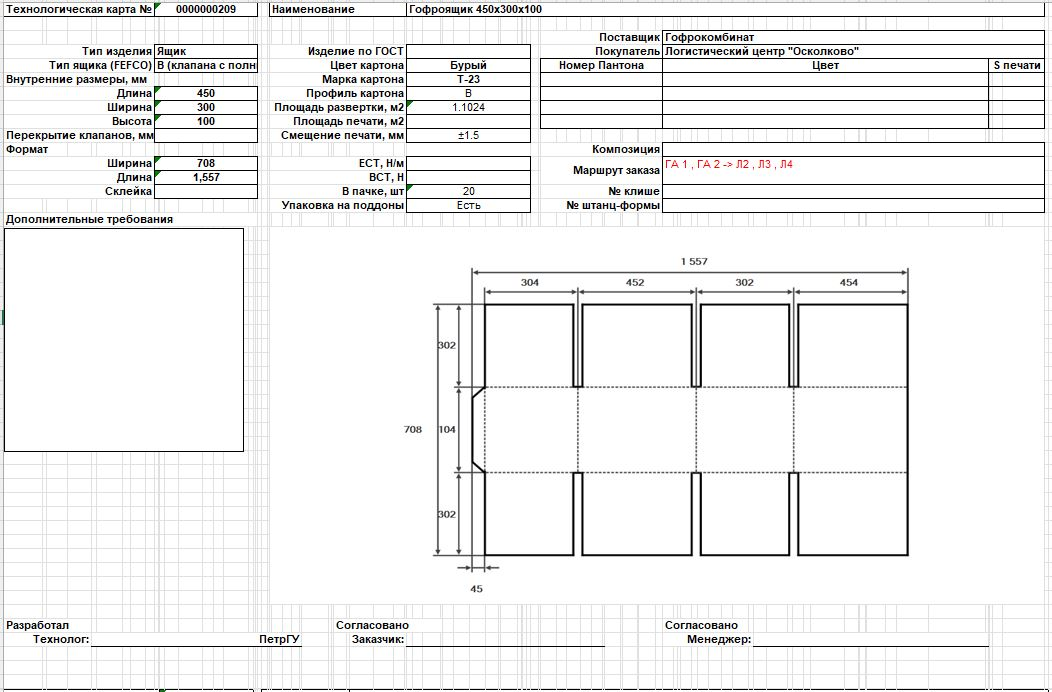
\includegraphics[height=0.8\textheight, width=\textwidth, angle=90,
  keepaspectratio] {50_Pics/Tk_1.JPG}
  \caption{Печатная форма Технологическая карта}
  \label{pic:Tk_1}
\end{figure}

\begin{figure}
\begin{center}
  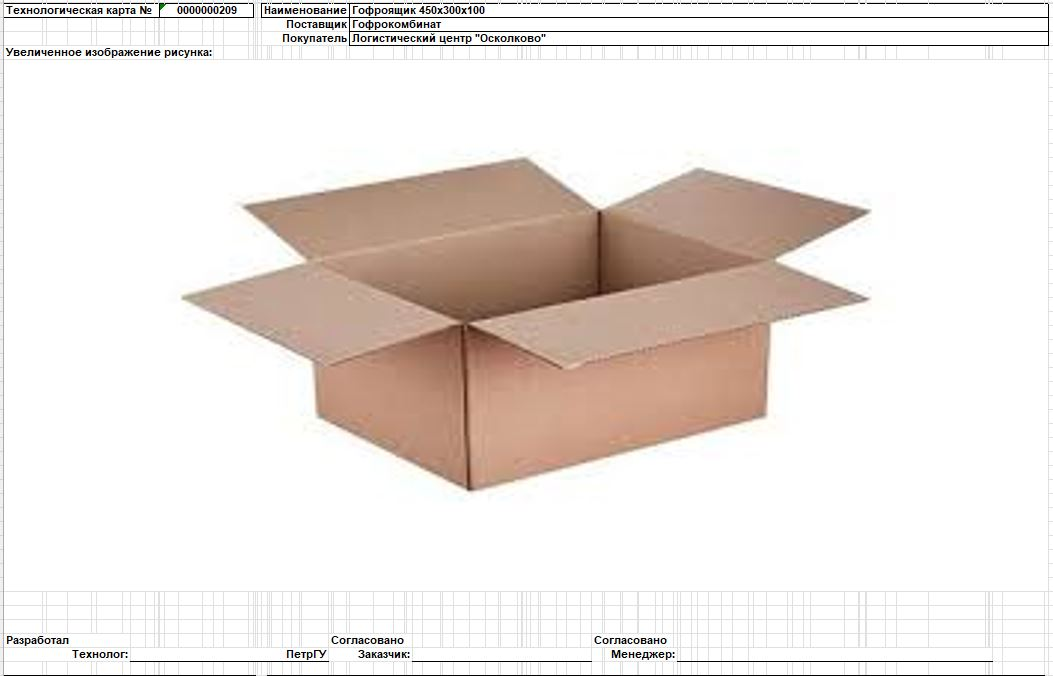
\includegraphics[height=0.7\textheight, width=\textwidth, angle=90,
  keepaspectratio]{50_Pics/Tk_2.JPG}
\end{center}
  \caption{Печатная форма Технологическая карта. Страница 2}
  \label{pic:Tk_2}
\end{figure}

\begin{figure}
\begin{center}
  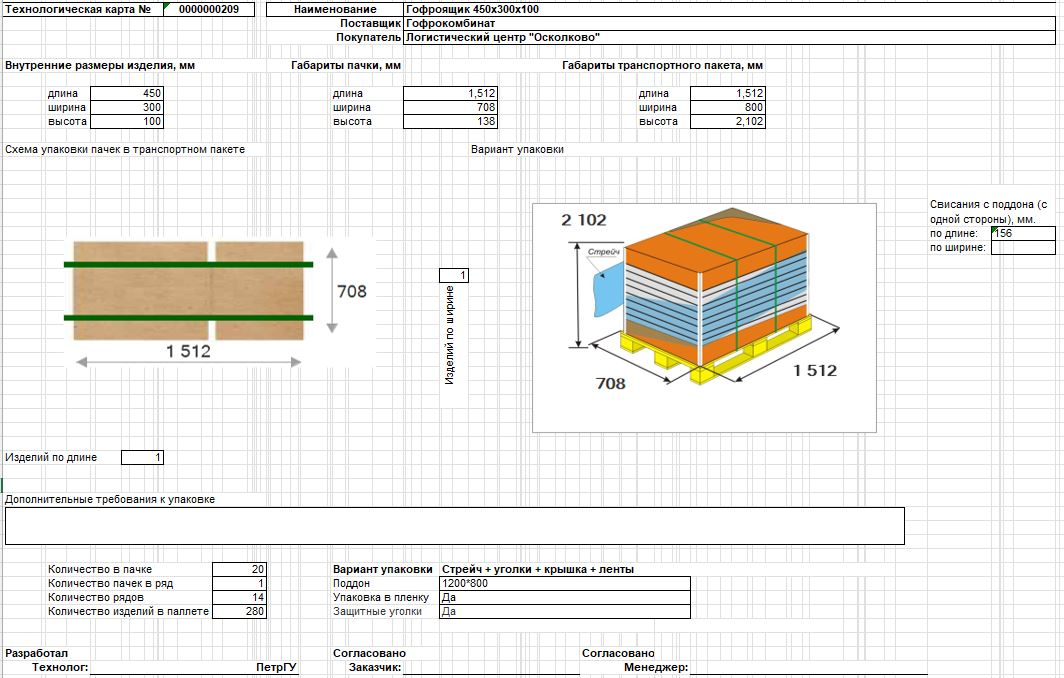
\includegraphics[height=0.7\textheight, width=\textwidth, angle=90,
  keepaspectratio]{50_Pics/Tk_3.JPG}
\end{center}
  \caption{Печатная форма Технологическая карта. Страница 3}
  \label{pic:Tk_3}
\end{figure}

\begin{figure}
\begin{center}
  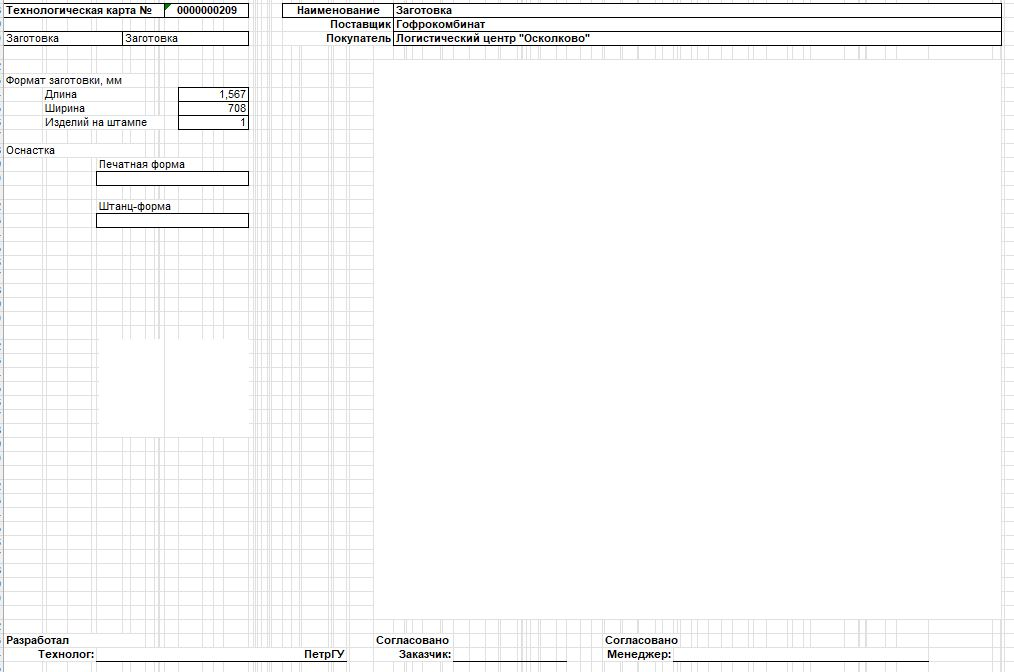
\includegraphics[height=0.7\textheight, width=\textwidth, angle=90,
  keepaspectratio]{50_Pics/Tk_4.JPG}
\end{center}
  \caption{Печатная форма Технологическая карта. Страница 4}
  \label{pic:Tk_4}
\end{figure}
\clearpage


\point{Форма ''Технологическая карта''. Вариант упаковки}

При выборе варианта упаковки заполнять реквизит ''Дно''.

% Форма уже существует в СИСТЕМЕ, требуется внести изменения в ее работу.



% \subsubsection{Функциональные требования}

% \point{Форма редактирования}

% (Точно нужно так перегружать???) Правило: Если ВесНетто = активен, доступно для редактирования поле <<Вес нетто>>, данные параметра <<Вес нетто>> выводить на бирку (Поле ВесНетто).
% Если ВесБрутто = активен, доступно для редактирования поле <<Вес брутто>>, данные параметра <<Вес брутто>> выводить на бирку (поле ВесБрутто).
% Если ВесНетто, ВесБрутто = неактивен, на бирке скрывать наименование полей ВесНетто и ВесБрутто. Пример бирки на готовую продукцию с отсутствием информации о весе нетто и брутто представлен на рис. \ref{pic:БиркаГП2}.


% %

% \input{20_Enums/spr_transconfitions}
% %%Справочник «Заготовки»
% %\input{10_Modules/Spr_billet.tex}
% %
% %%Справочник «Профили»
% %\input{10_Modules/Spr_Flute.tex}
% %
% %%Справочник Варианты упаковки
% \subsubsection{Справочник <<Варианты упаковки>>}
\label{spr:Rigging}
\renewcommand{\curobject}{<<Варианты упаковки>>>}

\point{Описание предметной области}

Справочник существует в СИСТЕМЕ, необходимо внести изменения в функциональность.

\point{Атрибуты}


Добавить новые атрибуты.
\pc
\begin{longtable}{|p{4cm}|p{4cm}|p{8cm}|}
\hline
{\bf Наименование} & {\bf Тип данных} &  {\bf Комментарий} \endhead
    \hline
    Дно & Флаг  & Признак необходимости добавления на дно прокладочных листов.\\
    \hline
  \caption{Новые поля Справочника \curobject}
 \label{tab:Design}
\end{longtable}



\point{Функциональные требования}


\subpoint{Редактирование справочника \curobject}

Добавить флаг в форму редактирвания

% Справочник должен быть доступен для редактирования пользователями с правами Дизайнер, Администратор, Менеджер. 
% %
% %
% % Справочник Оснастка
\subsection{Справочник <<Оснастка>>}
\label{spr:Rigging}
\renewcommand{\curobject}{<<Оснастка>>}

\subsubsection{Описание предметной области}

Справочник существует в СИСТЕМЕ, необходимо внести изменения в функциональность.

\subsubsection{Атрибуты}

\pc
\begin{longtable}{|p{40mm}|p{30mm}|p{12mm}|p{78mm}|}
\hline
{\bf Наименование} & {\bf Тип данных} &  {\bf Новое} &  {\bf Комментарий} \endhead
    \hline
   Комментарий  & Строка (неогр)  & Да & Текстовое описание комментария для оснастки \\
    \hline                    
   \caption{Поля справочника \curobject}
  \label{tab:Rigging}
\end{longtable}

 \point{Функциональные требования}

\subpoint{Команда ''Обновить''}

При использовании команд “Обновить” и “Обнулить” выдавать сообщение пользователю “Подтвердить выполнение: Да/Нет”.

\subpoint{Форма редактирования. Таблица объектов, ссылающихся на оснастку}

Добавить поле "Дата" для объектов типа "Документ". 
Сортировать документы по дате в порядке убывания.
% %
% Справочник Оборудование
\subsection{Справочник <<Оборудование>>}
\label{spr:eqpt}
\renewcommand{\curobject}{<<Оборудование>>}

\subsubsection{Описание предметной области}

Справочник \curobject содержит информацию о технологическом оборудовании на предприятии.

Справочник уже существует в СИСТЕМЕ, требуется внести изменения в его работу.

\subsubsection{Атрибуты}


\pc
\begin{longtable}{|p{50mm}|p{30mm}|p{78mm}|}
\hline
{\bf Наименование} & {\bf Тип данных} &  {\bf Комментарий} \endhead
\hline 
    Минимальная ширина заготовки & Число (4) & Минимальная ширина заготовки для оборудования типа Гофроагрегат  в мм\\
    \hline
    Минимальное расстояние между рилевками & Число (3) &  Минимальное расстояние между рилевками в мм \\
    \hline 
\caption{Описание новых полей справочника  \curobject}
\label{tab:eqpt}
\end{longtable}



\subsubsection{Функциональные требования}

% \point{Скорость гофроагрегата в зависимости от длины заготовки}


% %% Справочник Марки
% % \input{10_Modules/Spr_Mark.tex}

 %% Справочник Группы сложности
% \input{20_Enums/Spr_DiffGroup.tex}




	\section{Описание функций подсистемы <<Управление продажами>>}



% Документ  <<Предварительная калькуляция стоимости заказа>>} 
% \input{10_Modules/Doc_sales.tex}


% Документ  <<Заявка>>} 
% \input{10_Modules/Doc_Request.tex}

% Документ  <<Заказ>>} 
\subsection{Документ <<Заказ>>}
\label{doc:Order}
\renewcommand{\curobject}{<<Заказ>>}

\subsubsection{Описание предметной области}

Документ \curobject предназначен для регистрации производственного заказа на изготовление готовой продукции.

Документ существует в СИСТЕМЕ, необходимо добавить новую функциональность.


\subsubsection{Функциональные требования}


\point{Отображение информации о проблемах по заказу}

В форму заказа добавить новую вкладку <<Проблемы по заказу>>, в которой выводить записи для текущего заказа (если есть) из регистра <<Проблемы по заказам>>.

В таблице формы <<Проблемы по заказу>> выводить флаги из регистра сведений <<Проблемы по заказу>>:
\begin{itemize}
    \item В работе (да/нет); 
    \item Решено (да/нет)
\end{itemize}








%\subsection{Обработка <<Непрерывный план>>}
%
%\subsubsection{Функциональные требования}
%
%\point {Три разных заказа в одном раскрое}
%
%Предусмотреть, что бывает потребность выпустить в одном раскрое два заказа на одном столе и один на втором. При этом заказы на одном столе могут быть как одинаковые по длине, так и
%отличаться на заданную дельту. 
%
%
%\point {Печатная форма <<Раскрои (для выделенных)>>}
%
%При печати отчета заголовки таблицы выводить перед каждой группой раскроев.
%В заголовке группы раскроев оставить вывод информации по слоям только с требуемым количеством сырья.
%
%\begin{figure*}[!htb]
%\centering
%  \includegraphics[width=180mm, height=220mm, keepaspectratio]{10_Modules/Pics/picReportTaskGa.jpg}
%\caption{Печатная форма задания на гофроагрегат}
%\label{pic:picReportTaskGa}
%\end{figure*} 
%\FloatBarrier
%

%Регистр <<Проблемы по заказам>>
\subsection{Регистр <<Проблемы по заказам>>}
\label{reg:OrderError}

\subsubsection{Описание предметной области}

Регистр существует в системе, необходимо добавить новую функциональность.


\point{Атрибуты}


Добавить новые атрибуты.
\pc
\begin{longtable}{|p{4cm}|p{4cm}|p{8cm}|}
\hline
{\bf Наименование} & {\bf Тип данных} &  {\bf Комментарий} \endhead
    \hline
    В работе & Флаг  & Признак необходимости работы по проблеме.\\
    \hline
    Решено & Флаг  & Признак выполнения работы по проблеме.\\
    \hline
  \caption{Новые поля \curobject}
 \label{tab:Reg_OrderError}
\end{longtable}




% %Отчет <<Портфель заказов>>
% \input{10_Modules/Rep_OrderBag.tex} 
%  	\input{10_Modules/Mod_Plan.tex}
  	\section{Описание функций подсистемы <<Учет выработки на технологических линиях и гофроагрегате>>}


%Справочник «Оборудование»
%\input{10_Modules/Spr_Equipment.tex}

%  ********************                 Документы                   ********************************* 


%Документ «Выработка по переработке».
\subsection{Документ <<Выработка по переработке>>}
\label{doc:ProductionLine}



\subsubsection{Описание предметной области}

Документ существует в СИСТЕМЕ, необходимо добавить новую функциональность.
Документ участвует в процессе "Выпуск готовой продукции и полуфабрикатов".



\subsubsection{Функциональные требования}

\point{Исправить проверку выполнения задания}

При проверке выполнения данного задания, должна проверять  выполнение задания из значения ''Процент выпуска'' технологической карты заказа , а в случае если полученное значение равно «0» брать значение по умолчанию из настроек Системы.

% Документ  <<Выработка по гофроагрегату>>} 
\subsection{Документ <<Выработка гофроагрегата>>}
\label{doc:corrugatorproduction}



\subsubsection{Описание предметной области}

Документ существует в СИСТЕМЕ.
Документ предназначен для регистрации выработки заготовок и готовой продукции на гофроагрегате. Является рабочим местом оператора гофроагрегата.
Документ участвует в процессе "Выпуск готовой продукции и полуфабрикатов".



 \subsubsection{Функциональные требования}


\point{Исправить проверку выполнения задания}

При проверке выполнения данного задания, должна проверять  выполнение задания из значения ''Процент выпуска'' технологической карты заказа , а в случае если полученное значение равно «0» брать значение по умолчанию из настроек Системы.


\point{Печатать внутренней бирки}

Внутренняя бирка на заготовки должна печататься из СИСТЕМЫ.
За основу необходимо взять печатную форму СИСТЕМЫ и внести правки.
%привести к тому виду, который сейчас используется на ПРЕДПРИЯТИИ. 
Внешний вид внутренней бирки для заготовок представлен на рис. \ref{pic:InnerLabel}.

Бирки необходимо распечатать как для всех позиций выработки, так и для выделенных строк.

Бирка должна содержать следующие поля:
\begin{itemize}
    \item Номер заказа в СИСТЕМЕ;
    \item Наименование заготовки;
    % \item Размеры заготовки;
    \item Наименование номенклатуры готовой продукции;
    \item Контрагент;
    \item Дата производства, время начала выполнения заказа;
    % \item Оборудование;
    \item Номер смены.
    % \item Количество на паллете;
    % \item Марка + Профиль + Цвет.
\end{itemize}

%Реквизиты организации должны выводиться исходя из организации, указанной для заказа.

%На бирку (внутрицеховая) добавить время выпуска, номер (идентификатор) и № ярлыка по порядку с общим количеством ярлыков на этот заказ (например, 3 / 25). 
% На бирке выводить время печати (оно заменяет время выпуска, которое может быть еще неизвестно к моменту печати), идентификатор задания (из НП) и  № ярлыка с общим количеством ярлыков по данному раскрою (например, 3 из 25). Нумерация ярлыков должна идти с единицы для каждого раскроя с этим заказом (т.е., если будет два задания, то номера в бирках будут с единицы в обоих случаях).

\begin{figure*}[!htb]
\centering
  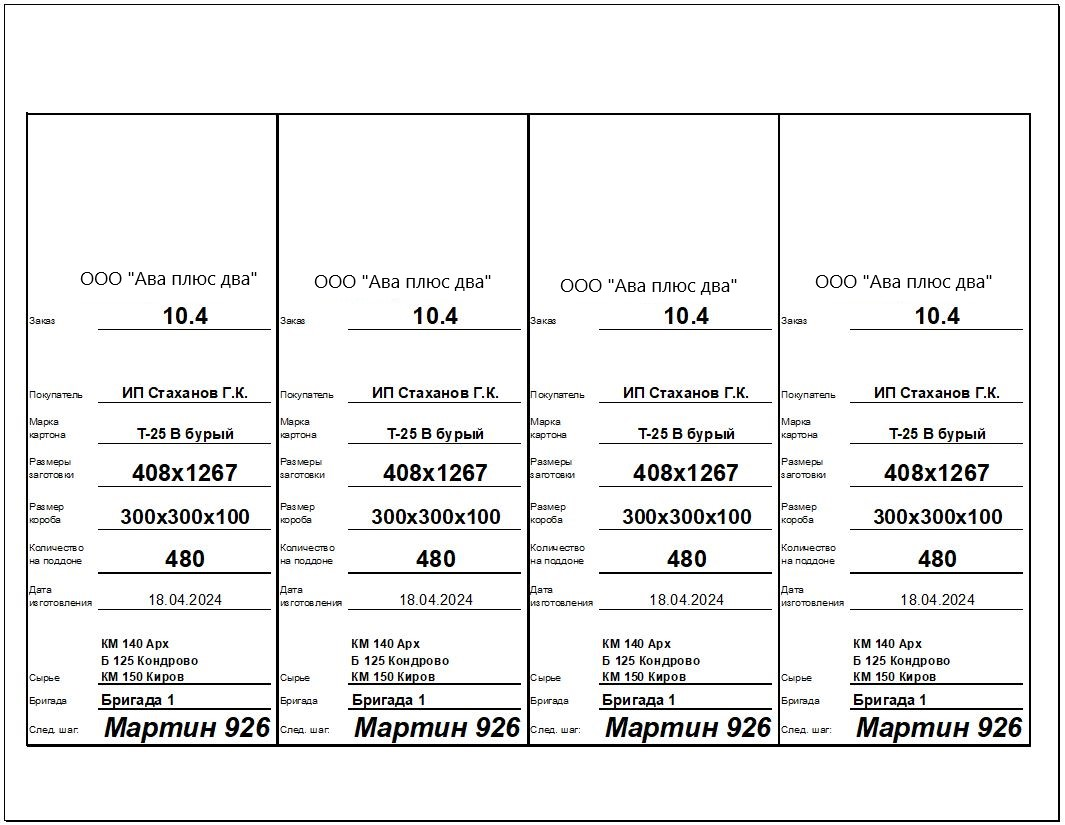
\includegraphics[width=140mm, height=220mm, keepaspectratio]{50_Pics/InnerLabel.JPG}
\caption{Пример внутренней бирки с гофроагрегата}
\label{pic:InnerLabel}
\end{figure*} 
\FloatBarrier







\point{Печать бирки на готовую продукцию}
\label{print:label}


Бирка на готовую продукцию (товарный гофрокартон) должна печататься из СИСТЕМЫ.
% %Добавить возможность печати бирок из СИСТЕМЫ.
% При печати бирок на готовую продукцию необходимо печатную форму привести к тому виду, который сейчас используется на ПРЕДПРИЯТИИ.

Пример бирки на товарный гофрокартон представлен на рис. \ref{pic:Label}.
% Графа с номером паллеты остается пустой и должна заполняться в распечатанном бланке упаковщиком.

% Реквизиты организации должны выводиться исходя из организации, указанной для заказа.
Бирка должна содержать следующие поля:
\begin{itemize}
    \item Наименование и адрес организации;
    % \item Логотип организации;
    \item Тип изделия. Значение определяется во типу продукции свойства ''Тип продукции'' в типе изделия технологической карты;
    \item Наименование номенклатуры;
    % \item Оборудование - оборудование последнего передела;
    \item Размер изделия;
    \item ГОСТ;
    \item Номер партии (??? не вывести);
    
    \item Бригада;
    % \item Цвет картона;
    % \item Марка картона;
    \item Количество на поддоне;
    \item Количество в кипе;
    \item Количество в партии;
    
    \item Штрих-код;
    % \item Манипуляционные знаки;
    % \item Количество на поддоне;
    % \item Количество подонов в заказе;
    % \item Марка картона;
    % \item Цвет картона;
    % \item Наименование линии;
    % \item Номер смены;
    \item Дата текущей выработки;
    % \item Дата первой выработки по заказу;
    % \item Номер заказа: Номер заказа в СИСТЕМЕ + Дата заказа + Номер заказа SAP + номер строки в SAP;
    % \item Номер паллеты в заказе;
    % \item Уникальный номер паллеты.
    % \item Тех.карта;
  %  \item Покупатель;
  %  \item Количество на поддоне;
  %  \item Бригада;
  %  \item Краткое наименование варианта упаковки, указанного в технологической карте.
\end{itemize}

Штрих-код на паллете должен определяться как номер заказа и количество продукции в паллете.


\begin{figure*}[!htb]
\centering
  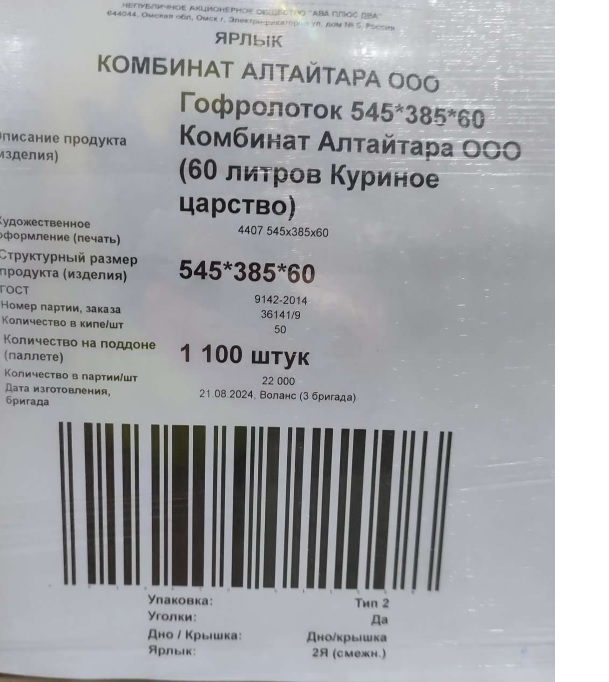
\includegraphics[width=140mm, height=220mm, keepaspectratio]{50_Pics/Label.jpg}
\caption{Пример бирки готовую продукцию}
\label{pic:Label}
\end{figure*} 
\FloatBarrier

% Поле <<Номер заказа в СИСТЕМЕ>> обозначено на примере цифрами 6693, поле <<Тех.карта>> обозначено на примере цифрами 1608.


ШК-код содержит строку формата: 
\begin{itemize}
    \item Код заказа 6 символов; % 4146500;
    % \item Символ ";"
    % \item "0000";
    % \item Первая часть номера заказа 6 знаков (номер заказа SAP);
    % \item Вторая часть заказа произвосдтва (номер строки в заказе SAP) 6 знаков с ведущими нулями;
    \item Количество на паллете 6 знаков с ведущими нулями;
    % \item Дата производства в формате ГГГГММДД.
\end{itemize}

Пример строки: 401465001100.


% Документ  <<Учет сырья на производстве>>} 
%\input{10_Modules/Doc_materialusing.tex}

%документ «Сырье для выработки»
%\input{30_Docs/Doc_LayersForProduction.tex}

%Отчет "Выработка за период"
% \input{40_Reports/Rep_OutputPeriod.tex}

%Отчет "Проблемы по заказу"
\subsection{Отчет <<Проблемы по заказу>>}
\label{rep:Rep_Problems}
\renewcommand{\curobject}{<<Проблемы по заказу>>}

Отчет существует в системе. Изменить работу отчета.

\subsubsection{Функциональные требования}

\point{Добавить новые колонки}

В табличную часть отчета добавить колонки:  “В работе” ; “Решено” из регистра 
''Проблемы по заказу''.

%Отчет "Простои оборудования (шахматка-полный)"
% \input{40_Reports/Rep_DowntimesEquipment.tex}
%	\input{10_Modules/Modules2.tex}
	\section{Описание функций подсистемы <<Планирование>>}



%  ********************                 Документы                   ********************************* 
%Документ «План».
\subsection{Документ <<План>>}
\label{doc:Plan}

\subsubsection{Описание предметной области}

Документ предназначен для составления планов работы гофроагрегата и перерабатывающего оборудования.

Документ существует в СИСТЕМЕ, необходимо внести изменения в функциональность.

При использовании механизма автоматического планирования работы гофроагрегата на предприятии увеличится количество раскроев, что приведет к разделению выхода паллет после гофроагрегата по одному заказу. 
Это потребует  организовать хранение паллет после гофроагрегата для удобного поиска паллет одного заказа. 

\subsubsection{Функциональные требования}

\point{Позаказный учет}

При внедрении СИСТЕМЫ ПРЕДПРИЯТИЕ должно перейти на планирование заданий и внесение выработки только с использованием номеров заказов менеджеров, не допускается (и невозможно) выдавать задания на номенклатуру без указания номера заказа.
Соответственно во многих формах и отчетах СИСТЕМЫ выводится не только номенклатура, но и номер заказа менеджера.

\point{Форма редактирования. Форма Редактирование раскроев}

В табличной части документа план изменить расположение колонок: 
Длина, ширина, рилевки.

\point{Форма редактирования. Вкладка ''Планирование линий''}

В табличной части документа план изменить расположение колонок: 
Длина, ширина.



\point{Печатная форма задания на гофроагрегат}

% Внести изменения в во внешний вид текущего задания, печатаемого из СИСТЕМЫ.
% \begin{itemize}
% \item Убрать колонку <<шт. изделий>>;
% \item Убрать колонку <<требуется изделий>>;
% \item Убрать колонку <<раскрой>>;
% \item Колонку <<Ширина>> заменить на <<Формат (полотна)>>;
% \item <<п.п>> (погонные метры) заменить на <<м2>>;
% \item переименовать <<\% потерь>> на <<\% обрези>>.
% \end{itemize}

% В печатном задании на ГА объем сырья надо учитывать с допуском (использовать коэффициенты гофрирования с браком из справочника ''Профили'').


%\point{Учет покупных заготовок}
%
%
%При построении раскроев уменьшать количество заготовок у заказов на величину, указанную в атрибуте ''КоличествоПокупныхЗаготовок''.
%Объем для кроя должен быть взят за минусом заготовок, которые пользователь с ролью !Плановик решил заказать на стороне и не выпускать на гофроагрегате.




\subsection{Обработка <<Непрерывный план>>}
\label{doc:PlanInfinite}

\subsubsection{Функциональные требования}

% Добавить из Архбум

\point {Гофроагрегат. Подсветка заданий}

Добавить подсветку раскроев в форме непрерывного плана.
Подсвечивать строки как для раскроев с разными типами рилевок для сделующих случаев.
Менее значения параметра «Минимальное расстояние между рилевками» одно из следующего:
\begin{itemize}
    \item 
 расстояние между рилевками внутри изделия (проверяется для каждого заказа раскроя)
\item  Сумма значений крайних рилевок двух разных заказов из раскроя (если в раскрое есть два заказа). Пусть рилевки первого заказа A1/A2/A3, а рилевки второго заказа B1/B2/B3, тогда надо проверить A1+B3 и A3+B1
\item   Двойное значение каждой из крайних рилевок, если заказ в раскрое идет более чем одной полосой. Для обозначений выше это означает проверку 2*A1 и 2*A
\end{itemize}

% \point {Отображение проблем по заказам}

% Добавить вывод колонки <<Проблемы>>, ячейка которой должна быть закрашена красным цветом, если для данного заказа имеются записи в регистре <<Проблемы по заказам>> --- это будет сигналом для плановика, что необходимо открыть форму заказа и просмотреть список проблем. 


\point{Исправить проверку выполнения задания}

В непрерывном плане при проверке выполнения данного задания, должна проверять  выполнение задания из значения ''Процент выпуска'' технологической карты заказа , а в случае если полученное значение равно «0» брать значение по умолчанию из настроек Системы.


\point{Добавить команду разделения заказов}

В форме «Непрерывный план» для табличной части плана по линиям переработки в контекстное меню необходимо добавить функцию разделения задания. При выборе пользователем данной команды должна быть открыта дополнительная форма, в которой пользователь должен указать объем, остающийся в первой части задания, а Система должна автоматически рассчитать количество для отделяемой части как разницу между объемом задания и объемом первой части.


\point{Печатать форму ТК}

Изменить вызов печатной формы в ТК в таблице заказов на печать полной формы ТК.


% \input{40_Reports/Rep_NPPlan.tex}
	% \section{Описание функций подсистемы <<Склады>>}



%  ********************                 Документы                   ********************************* 


%Документ «Реализация ТМЦ».
\input{30_Docs/Doc_Realization.tex}
%	
%	\input{10_Modules/Mod_OPCExchange.tex}

 	\newpage

\section{Требования к правилам обмена с системой 1С:УПП.}
\label{sec:exchange}

%Схема обмена по передаче параметров для планирования между 1С:УПП и СИСТЕМОЙ представлена на рисунке \ref{pic:exchange}.
%
%
%\subsection{Справочник ''Номенклатура''}
%
%\subsection{Обмен документом ''Установка цен номенклатуры''}
%






\subsection{Функциональные требования}

\subsubsection{Первоначальная выгрузка}


Необходимо организовать первоначальную выгрузку справочников из 1С:УПП в СИСТЕМУ.
% На Предприятии учет реализован в нескольких информационных базах 1С: Бухгалтерия.

%В последующем необходимо по расписанию выгружать эти справочники из 1С:УПП в Гофротару.

%Справочник <<Типы цен>> передаваться между системами не должен. 

\begin{itemize}
   \item Номенклатура --- загрузить из справочника ''Номенклатура'' согласно правил обмена;
  \item Контрагент --- загрузить полностью из справочника ''Контрагент'';
  \item Договоры контрагентов --- загрузить полностью из справочника ''Договоры контрагентов'';
%   \item Причины брака --- загрузить полностью из справочника  ''Причины брака''.
%   \item Причины остановов --- загрузить полностью из справочника  ''Причины остановов''.
% \item Спецификации номенклатуры --- загрузить согласно правил обмена.

%   \item Единицы измерения --- загрузить полностью из справочника ''Единицы измерения'';
%   \item Ставки НДС --- загрузить полностью из справочника ''Ставки НДС'';
%   \item Структурные единицы --- загрузить полностью из справочника ''Места хранения'';
%   \item Организации --- загрузить полностью из справочника ''Организации'';
%   \item Банки --- загрузить полностью из справочника ''Банки'';
 % \item Сотрудники --- загрузить полностью из справочника ''Банковские счета''.
 \item Физические лица --- загрузить полностью из справочника ''Физические лица''.
% \item Технологические карты --- загрузка полностью из справочника ''Номенклатура'' и ''Характеристика номенклатуры''.
\end{itemize}




  % Первоначальная загрузка справочника ''Номенклатура'' должна быть выполнена по следующему отбору.
% % Table generated by Excel2LaTeX from sheet '1С'
% \scriptsize
% \begin{longtable}{|p{20mm}|p{70mm}|p{64mm}|}
% \hline
% {\bf \parbox[c][15mm]{20mm}{\centeringКод группы}} & {\bf \parbox[c]{70mm}{\centeringПуть}} & \parbox[c]{64mm}{\centeringМатериалы (справочно)} \\
% \hline
% \parbox[c][5mm]{30mm}{00000000067} & Номенклатура-Материалы-Сырье и материалы (10-1) & сырье (бумага, картон) \\
% \hline
% \parbox[c][30mm]{30mm}{00000002884} & Номенклатура-Материалы-Прочие материалы-Сопутствующие & крахмал, едкий натр, бура
% прочие хим.добавки
% клей ПВА
% ленты ПП и ПЭ, скобы, скотч
% стрейч-пленка \\
% \hline
% \parbox[c][9mm]{30mm}{БП-00000989} & Номенклатура-Материалы-Прочие материалы-Покупной гофрокартон & покупной гофрокартон \\
% \hline
% \parbox[c][9mm]{30mm}{00000002632} & Номенклатура-Материалы-Прочие материалы-Флексоформы & оснастка (штанцевые и печатные формы) \\
% \hline
% \parbox[c][5mm]{30mm}{БП-00000996} & Номенклатура-Материалы-Прочие материалы-Краска & флексо-краска \\
% \hline
% \caption{Отбор справочника ''Номенклатура'' для первоначальной загрузки}\label{taB:nomload}
% \end{longtable}  
% \normalsize



\subsubsection{Регулярный обмен}
\label{exchange:regular}
Регулярный обмен между системами 1С: УПП и OPTI-CORRUGATED должен быть настроен по регламентному заданию. Время и периодичность выполнения должны быть заданы в обеих базах.

Механизм обмена - Web-сервис, План обмена.

При обмене с системой 1С: УПП загруженные документы не должны проводиться.

Структура обмена по учету производства представлена на рис. \ref{pic:DFD}.

\begin{figure}[htb]
\begin{center}
   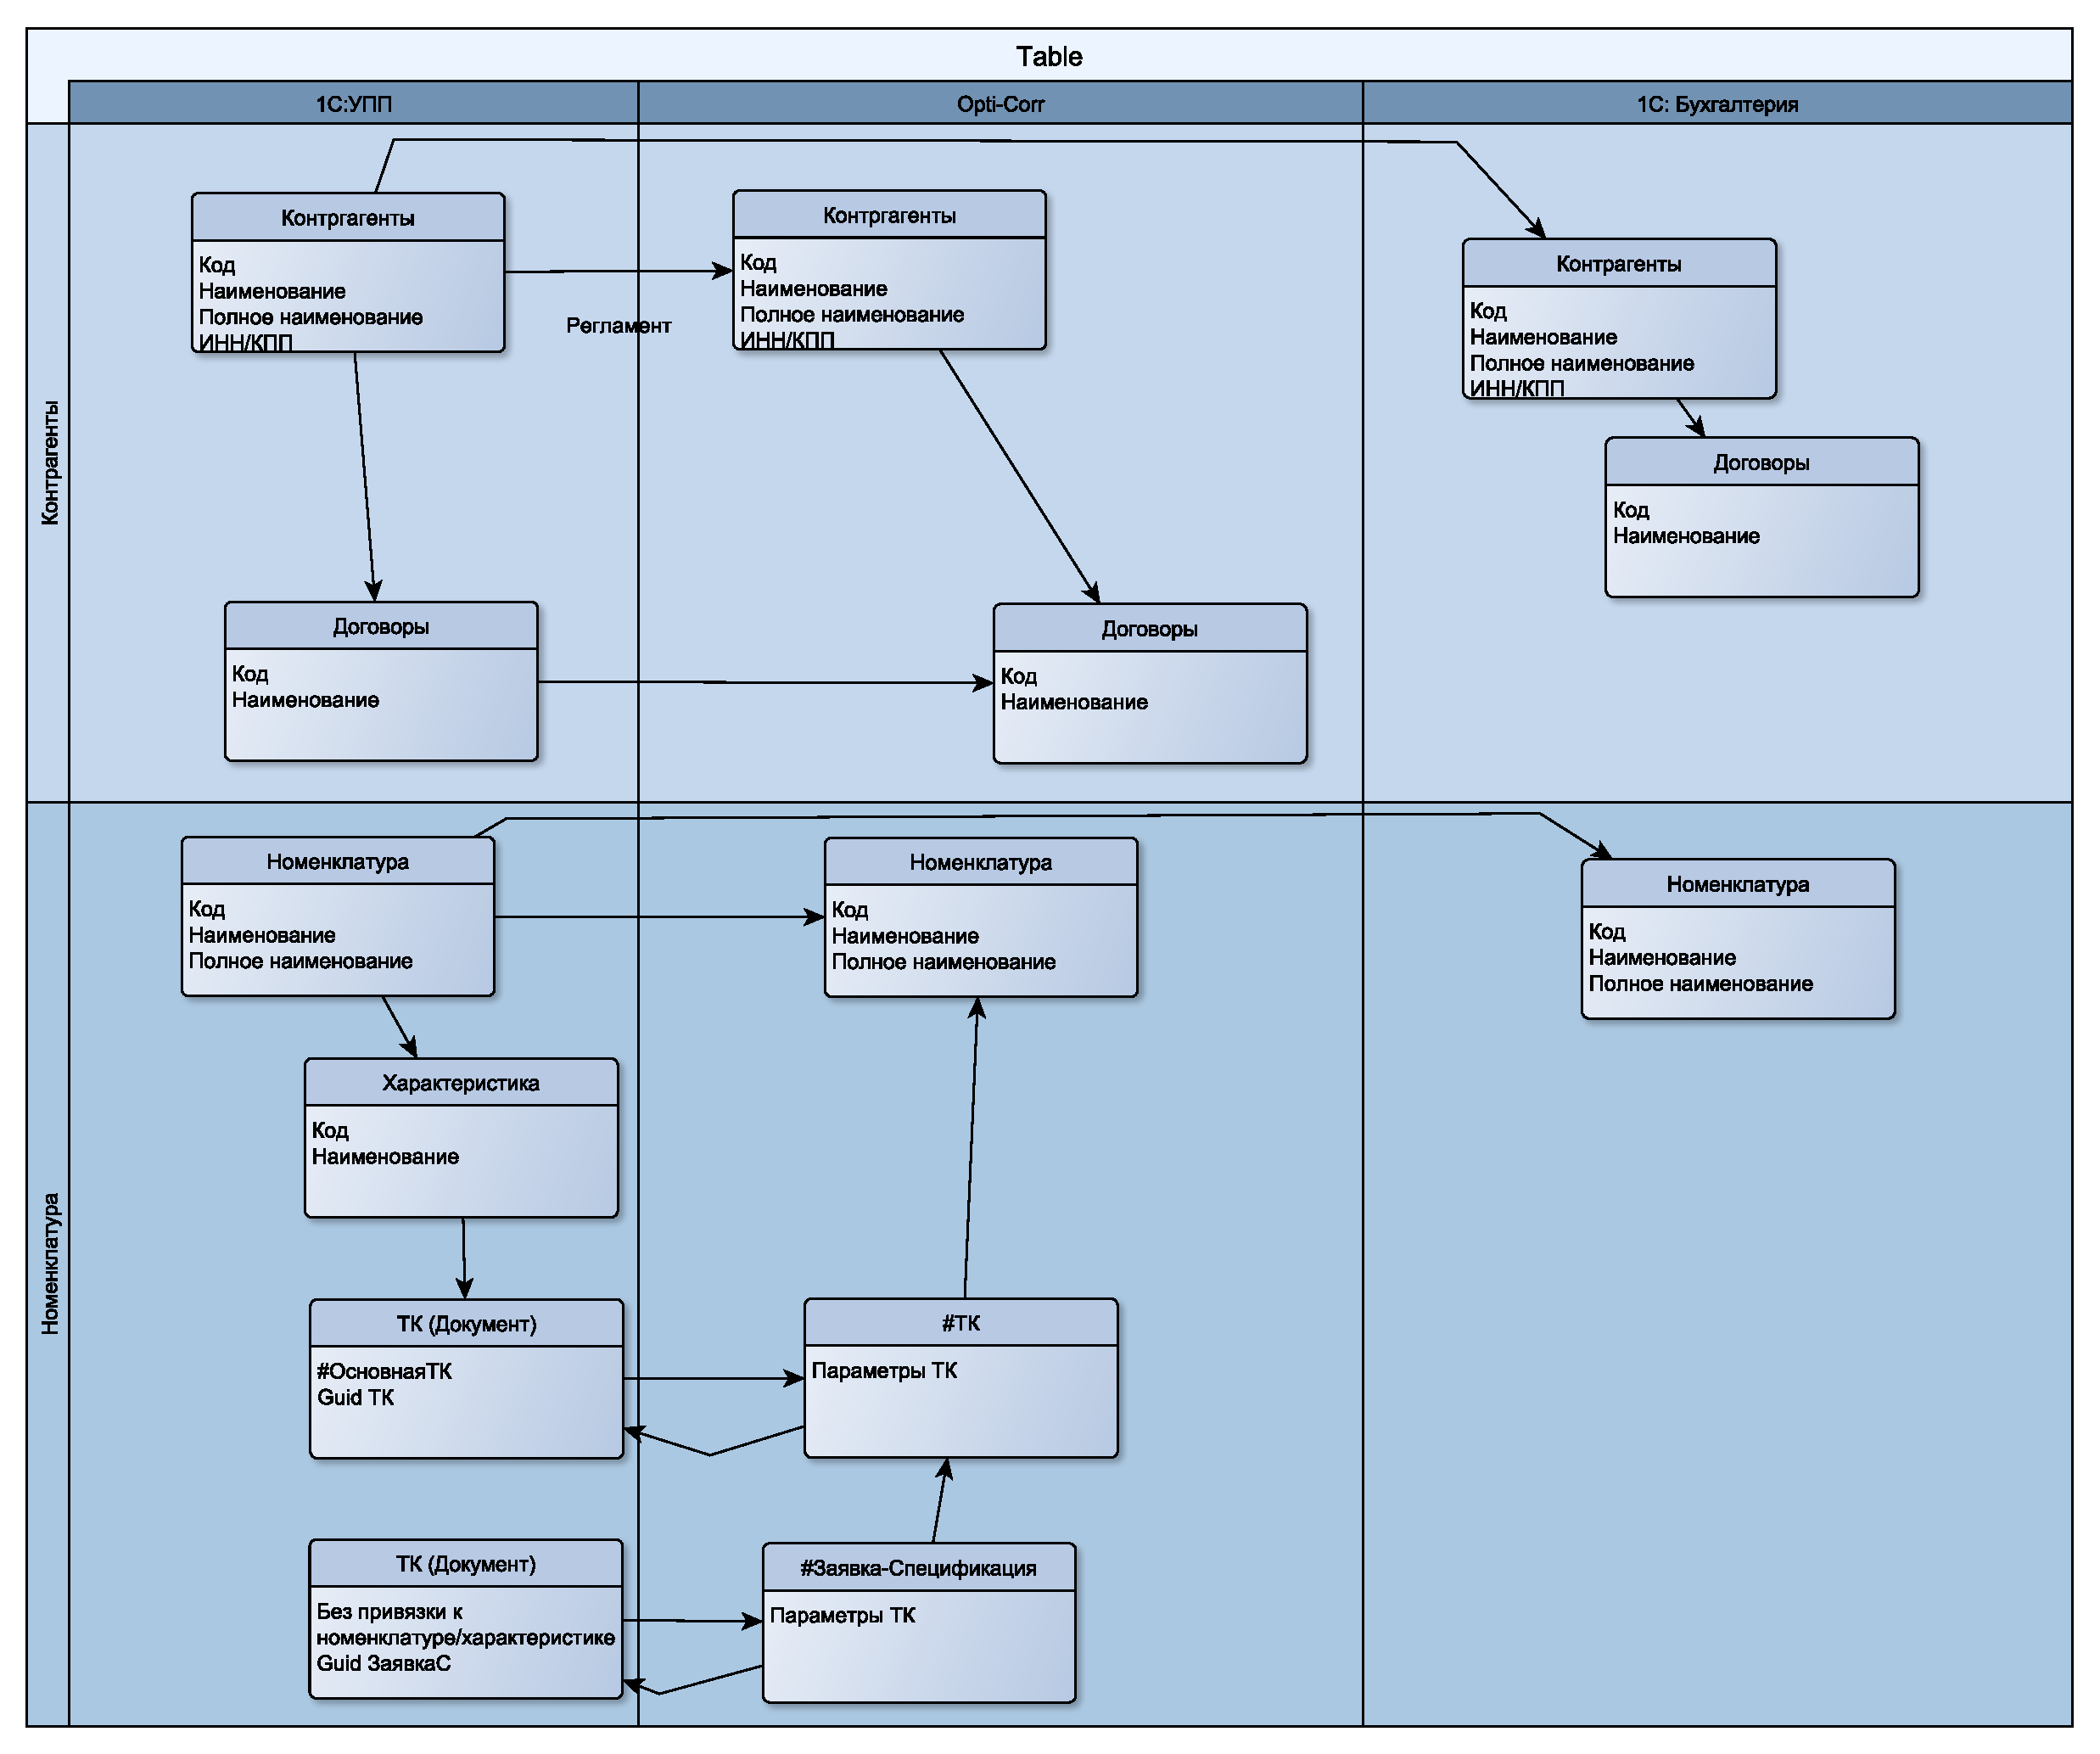
\includegraphics[height=0.8\textheight, width=1\textwidth, angle=0,  keepaspectratio]{50_Pics/DFD.pdf}
\end{center}
   \caption{Потоки обмена информацией между системами. НСИ}
   \label{pic:DFD}
\end{figure}
\FloatBarrier

\begin{figure}[htb]
\begin{center}
  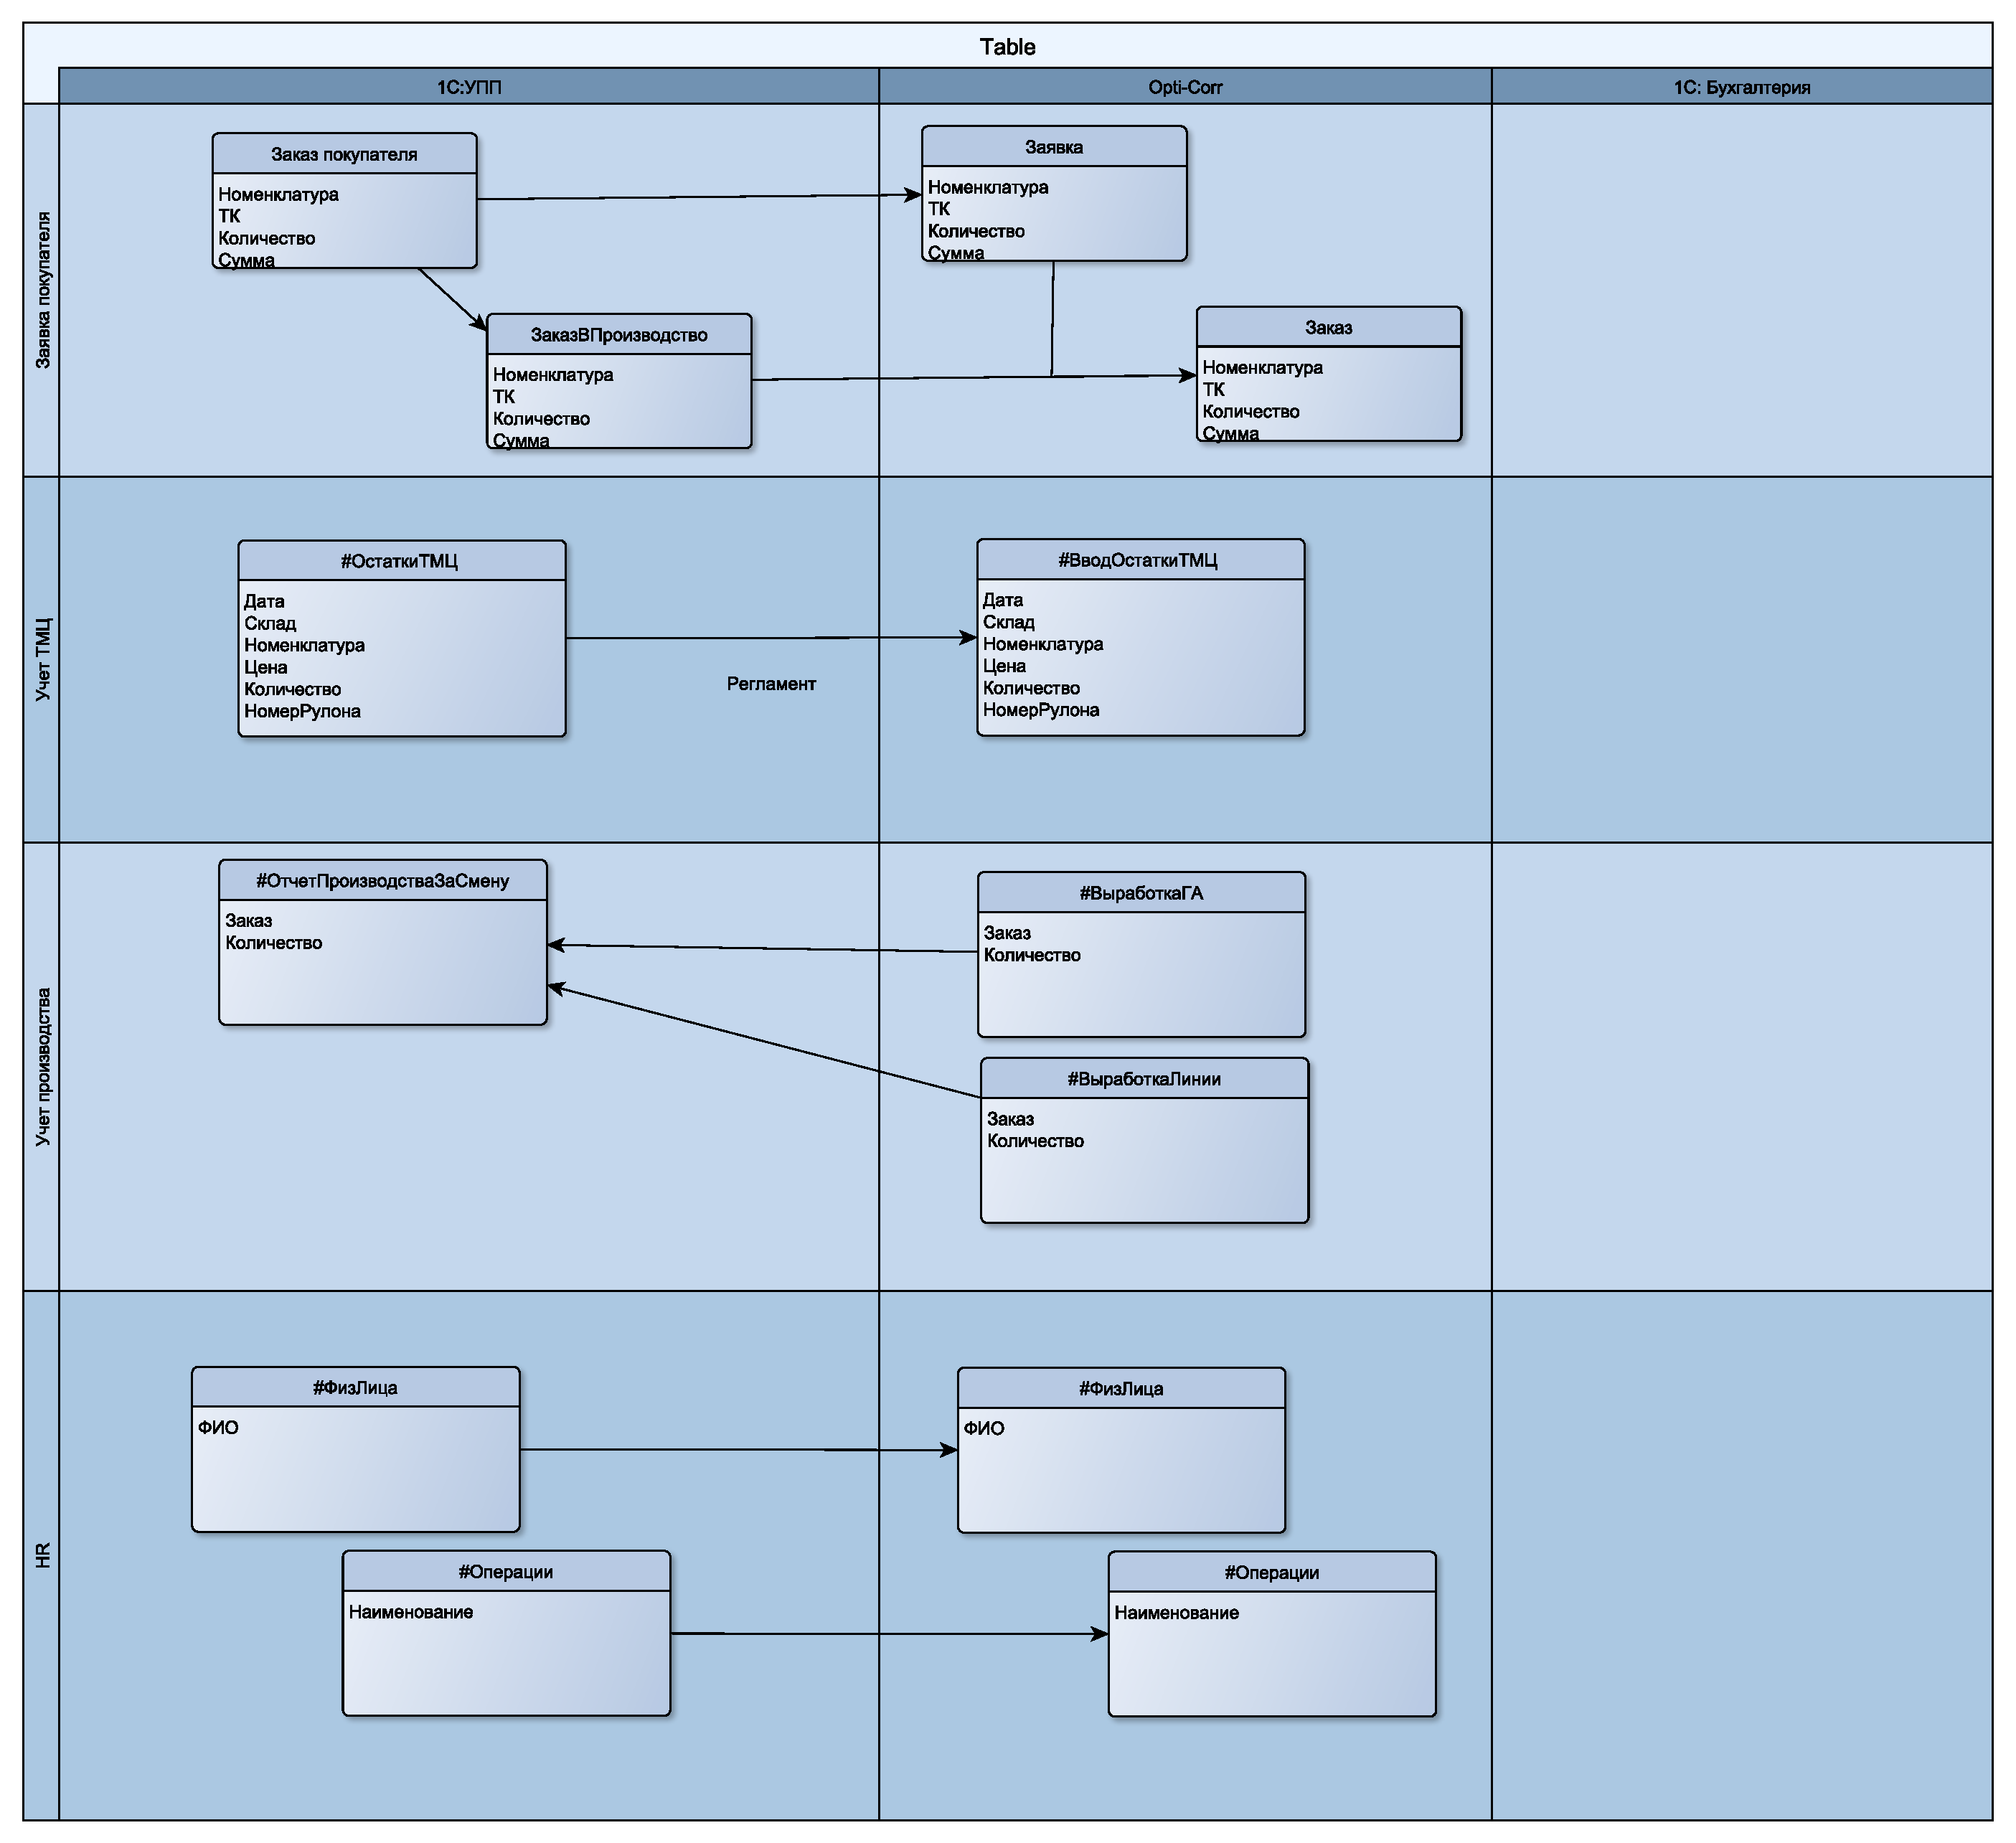
\includegraphics[height=0.8\textheight, width=1\textwidth, angle=0,  keepaspectratio]{50_Pics/DFD_2.pdf}
\end{center}
  \caption{Потоки обмена информацией между системами. Учет ТМЦ и готовой продукции}
  \label{pic:DFD_2}
\end{figure}
\FloatBarrier



% Table generated by Excel2LaTeX from sheet 'Лист1'
% \scriptsize
\begin{longtable}{|p{70mm}|p{70mm}|}
\hline
\parbox[c][19mm]{55mm}{\centering Документ 1С:УПП. Источник} & \parbox[c]{55mm}{\centering Документ Гофротары. Получатель}  \\
\hline
\parbox[c][6mm]{60mm}{Заказ покупателя} & Заявка \\
\hline
\parbox[c][6mm]{60mm}{Заказ производства} & Заказ  \\
\hline
\parbox[c][12mm]{60mm}{Остатки ТМЦ. Остатки по регистру на дату} & Ввод остатков ТМЦ  \\
\hline
\caption{Соответствие между документами для обмена}\label{tab:exchange2}
\end{longtable}  
\normalsize




% Table generated by Excel2LaTeX from sheet 'Лист1'
% \scriptsize
\begin{longtable}{|p{70mm}|p{70mm}|}
\hline
\parbox[c][19mm]{55mm}{\centering Документ Гофротары. Источник} & \parbox[c]{55mm}{\centering Соответствующий документ 1С:УПП. Получатель}  \\
\hline
\parbox[c][6mm]{60mm}{Выработка ГА} & Отчет производства за смену \\
\hline
\parbox[c][6mm]{60mm}{Выработка линии} & Отчет производства за смену \\
\hline
\caption{Соответствие между документами для обмена}\label{tab:exchange3}
\end{longtable}  
\normalsize


% \textbf{Выгрузка из OPTI-CORRUGATED в 1С: Бухгалтерия предприятия. Остатки ТМЦ}

% Источник: OPTI-CORRUGATED.

% Получатель: 1С: Бухгалтерия.

% По регламенту ежедневно в 8 утра либо принудительно по запросу необходимо из системы 1С: УПП выгружать текущие остатки по всем складам по слоям картона (Вид номенклатуры - Материалы).

% В СИСТЕМУ информация должна загружаться через вызов WEB-сервиса LoadData.

% Структура обмена


\point{Создать правило загрузки справочника ''Номенклатура'' в СИСТЕМУ}

Создать правило выгрузки из 1C: УПП в СИСТЕМУ справочника ''Номенклатура''.


Описание.

По регламенту необходимо выгружать зарегистрированные в плане обмена элементы справочника ''Номенклатура'' в части готовой продукции, номенклатуры сырья и оснастки из 1С: УПП в СИСТЕМУ.

Т.к. в 1С: УПП номенклатура ведётся в разрезе характеристик, то при передаче в СИСТЕМУ будет создано столько элементов справочника ''Номенклатура'', сколько заведено характеристик в объекте-источнике. При этом передаваемая в СИСТЕМУ номенклатура формируется по принципу ''Номенклатура + Характеристика'', и будет содержать два родительских GUID для дальнейшей синхронизации.

Синхронизация групп справочника выполняется по GUID соответствущей группы-номенклатуры.

Источник: 1С: УПП.

Объекты-источники: Номенклатура, Характеристики номенклатуры

Получатель: СИСТЕМА.

Объект получателя: Номенклатура

Параметры запроса:

% Table generated by Excel2LaTeX from sheet '20'
\scriptsize
\pc

\begin{longtable}{|p{10mm}|p{35mm}|p{40mm}|p{60mm}|}
\hline
\parbox[c][5mm]{10mm}{\centering№} & \parbox[c]{35mm}{\centeringНазвание параметра} & \parbox[c]{40mm}{\centeringТип значения} & \parbox[c]{60mm}{\centeringОписание} \\
\hline
\parbox[c][5mm]{16mm}{\p} &  GUID Номенклатуры & Уникальный идентификатор &         \\
\hline
\parbox[c][5mm]{16mm}{\p} &  GUID Характеристики & Уникальный идентификатор & Для групп не передаётся \\
\hline
%\parbox[c][5mm]{16mm}{\p} &  Код &     Строка &        Код \\
%\hline
\parbox[c][5mm]{16mm}{\p} & Наименование &     Строка & Наименование \\
\hline
\parbox[c][5mm]{16mm}{\p} & ПометкаУдаления & Булево & \\
\hline
\parbox[c][5mm]{16mm}{\p} & Полное наименование &     Строка & Полное наименование \\
\hline
\parbox[c][5mm]{16mm}{\p} & Родитель & Справочник ''Номенклатура'' & Группа \\
\hline
\parbox[c][5mm]{16mm}{\p} & GUID Тех. карты & Уникальный идентификатор & Передаётся для номенклатуры готовой продукции \\
\hline
%\parbox[c][5mm]{16mm}{\p} & Характеристика &     Строка & Характеристика номенклатуры \\
%\hline

% \parbox[c][5mm]{16mm}{\p} & Цены & Таблица Значений &            \\
% \hline
% \parbox[c][5mm]{16mm}{} & Тип цены &     Строка & Строка типа цены \\
% \hline
% \parbox[c][5mm]{16mm}{} & Дата &     Строка & Выгружается на последнюю дату изменения \\
% \hline
% \parbox[c][5mm]{16mm}{} & Значение &     Строка & Значение цены \\
% \hline
\caption{Параметры обмена справочника ''Номенклатура''}\label{ex:nomenclature}
\end{longtable}  
\normalsize

%\clearpage




\point{Создать правило загрузки справочника ''Контрагенты'' в СИСТЕМУ}

Создать правило выгрузки из 1C: УПП в СИСТЕМУ справочника ''Контрагенты''.


Описание.

По регламенту необходимо выгружать зарегистрированные в плане обмена элементы справочника ''Контрагенты'' из 1С:УПП в СИСТЕМУ.

% Синхронизация выполняется по полям ''ИНН'' и ''КПП''. В случае, если данные поля не заполнены, поиск будет осуществляться по полю ''Наименование''.
Синхронизация выполняется по GUID.

Источник: 1С:УПП.

Получатель: СИСТЕМА.

Параметры запроса:
\pc
% Table generated by Excel2LaTeX from sheet '20'
\scriptsize
\begin{longtable}{|p{10mm}|p{35mm}|p{40mm}|p{60mm}|}
\hline
\parbox[c][5mm]{10mm}{\centering№} & \parbox[c]{35mm}{\centeringНазвание параметра} & \parbox[c]{40mm}{\centeringТип значения} & \parbox[c]{60mm}{\centeringОписание} \\
\hline
\parbox[c][5mm]{16mm}{\p} &  GUID &  Уникальный идентификатор & Уникальный идентификатор \\
\hline
\parbox[c][5mm]{16mm}{\p} & Наименование &     Строка & Наименование \\
\hline
\parbox[c][5mm]{16mm}{\p} & ПометкаУдаления & Булево & \\
\hline
\parbox[c][5mm]{16mm}{\p} & Наименование полное &     Строка & Наименование полное \\
\hline
\parbox[c][5mm]{16mm}{\p} &   Родитель &  Справочник ''Контрагенты'' & Группа \\
\hline
\parbox[c][5mm]{16mm}{\p} &        ИНН &     Строка &        ИНН \\
\hline
\parbox[c][5mm]{16mm}{\p} &        КПП &     Строка &        КПП \\
\hline
\parbox[c][5mm]{16mm}{\p} & Код по ОКПО &     Строка &   Код по ОКПО \\
\hline
\parbox[c][5mm]{16mm}{\p} & Юр. / физ. лицо &  Перечисление & Юр. / физ. лицо  \\
\hline
\parbox[c][5mm]{16mm}{\p} & Основной договор & Справочник ''Договоры контрагентов'' & Основной договор контрагента \\
\hline
% \parbox[c][5mm]{16mm}{6} & Номер счета &     Строка & Номер счета \\
% \hline
% \parbox[c][5mm]{16mm}{7} &    Код БИК &     Строка &    Код БИК \\
% \hline
\caption{Параметры обмена справочника ''Контрагенты''}\label{ex:customer}
\end{longtable}  
\normalsize




\point{Создать правило загрузки справочника ''Договоры контрагентов'' в СИСТЕМУ}

Создать правило выгрузки из 1C: УПП в СИСТЕМУ справочника ''Договоры контрагентов''.


Описание.

По регламенту необходимо выгружать зарегистрированные в плане обмена элементы справочника ''Договоры контрагентов'' из 1C: УПП в СИСТЕМУ.

%Синхронизация выполняется по полям ''Номер договора'', ''Дата договора'' и ''Владелец'' (Контрагент).
Синхронизация выполняется по GUID.

Источник: 1С: УПП.

Получатель: СИСТЕМА.

Параметры запроса:
\pc
% Table generated by Excel2LaTeX from sheet '20'
\scriptsize
\begin{longtable}{|p{10mm}|p{35mm}|p{40mm}|p{60mm}|}
\hline
\parbox[c][5mm]{10mm}{\centering№} & \parbox[c]{35mm}{\centeringНазвание параметра} & \parbox[c]{40mm}{\centeringТип значения} & \parbox[c]{60mm}{\centeringОписание} \\
\hline
\parbox[c][5mm]{16mm}{\p} & GUID & Уникальный идентификатор & Уникальный идентификатор \\
\hline
\parbox[c][5mm]{16mm}{\p} & Наименование &  Строка & Наименование \\
\hline
\parbox[c][5mm]{16mm}{\p} & ПометкаУдаления & Булево & \\
\hline
\parbox[c][5mm]{16mm}{\p} & Владелец & Справочник ''Контрагенты'' & Контрагент \\
\hline
\parbox[c][5mm]{16mm}{\p} & Номер & Строка & Номер договора \\
\hline
\parbox[c][5mm]{16mm}{\p} & Дата & Строка & Дата договора \\
\hline
\parbox[c][5mm]{16mm}{\p} & Вид договора & Перечисление & Вид договора \\
\hline
\parbox[c][5mm]{16mm}{\p} & Организация &  Справочник ''Организации'' & Организация \\
\hline
\parbox[c][5mm]{16mm}{\p} & Тип цен &  Справочник ''Типы цен'' & Тип цен \\
\hline
\parbox[c][5mm]{16mm}{\p} & Валюта &  Справочник ''Валюты'' & Валюта взаиморасчётов \\
\hline
\parbox[c][5mm]{16mm}{\p} & СуммаКредита & Число & Допустимая сумма задолженности \\
\hline
\parbox[c][5mm]{16mm}{\p} & СрокКредита & Число & Допустимое число дней задолженности \\
\hline
\parbox[c][5mm]{16mm}{\p} & КонтролироватьКредит & Булево & Контролировать число дней задолженности \\
\hline
% \parbox[c][5mm]{16mm}{3} & Валюта взаиморасчетов &     Справочник ''Валюты'' & Валюта договора \\
% \hline
% \parbox[c][5mm]{16mm}{3} & Срок кредита & Число & Допустимое число дней задолженности \\
% \hline
% \parbox[c][5mm]{16mm}{3} & Сумма кредита & Число & Допустимая сумма задолженности \\
%\hline

\caption{Параметры обмена справочника ''Договоры контрагентов''}\label{ex:contract}
\end{longtable}  
\normalsize



\point{Создать правило загрузки справочника ''Склады'' в СИСТЕМУ}

Создать правило выгрузки из 1C: УПП в СИСТЕМУ справочника ''Склады''.


Описание.

По регламенту необходимо выгружать зарегистрированные в плане обмена элементы справочника ''Склады'' из  1C: УПП в СИСТЕМУ.

%Синхронизация выполняется по полям ''Код''.
Синхронизация выполняется по GUID.

Источник: 1С: УПП.

Объект-источник: Справочник ''Склады'' 

Получатель: СИСТЕМА.

Объект-получатель: Справочник ''Структурные единицы''

Параметры запроса:
\pc
% Table generated by Excel2LaTeX from sheet '20'
\scriptsize
\begin{longtable}{|p{10mm}|p{35mm}|p{40mm}|p{60mm}|}
\hline
\parbox[c][5mm]{10mm}{\centering№} & \parbox[c]{35mm}{\centeringНазвание параметра} & \parbox[c]{40mm}{\centeringТип значения} & \parbox[c]{60mm}{\centeringОписание} \\
\hline
\parbox[c][5mm]{16mm}{\p} & GUID & Уникальный идентификатор & Уникальный идентификатор \\
\hline
\parbox[c][5mm]{16mm}{\p} & Наименование &     Строка & Наименование \\
\hline
\parbox[c][5mm]{16mm}{\p} & ПометкаУдаления & Булево & \\
\hline
% \hline
% \parbox[c][5mm]{16mm}{3} & Валюта взаиморасчетов &     Справочник ''Валюты'' & Валюта договора \\
% \hline
% \parbox[c][5mm]{16mm}{3} & Срок кредита & Число & Допустимое число дней задолженности \\
% \hline
% \parbox[c][5mm]{16mm}{3} & Сумма кредита & Число & Допустимая сумма задолженности \\
% \hline

\caption{Параметры обмена справочника ''Склады''}\label{ex:contract}
\end{longtable}  
\normalsize


\point{Создать правило загрузки справочника ''Физические лица'' в СИСТЕМУ}

Создать правило выгрузки из СИСТЕМЫ из  1C: УПП в СИСТЕМУ справочника ''Физические лица''.

% СправочникСсылка.ФизическиеЛица
Описание.

По регламенту необходимо выгружать зарегистрированные в плане обмена элементы справочника ''Физические лица'' из 1C: УПП в СИСТЕМУ.

%Синхронизация выполняется по полям ''Код''.
Синхронизация выполняется по GUID.

Источник: 1С: УПП.

Объект-источник: Справочник ''Физические лица'' 

Получатель: СИСТЕМА.

Объект-получатель: Справочник ''Физические лица''

Параметры запроса:
\pc
% Table generated by Excel2LaTeX from sheet '20'
\scriptsize
\begin{longtable}{|p{10mm}|p{35mm}|p{40mm}|p{60mm}|}
\hline
\parbox[c][5mm]{10mm}{\centering№} & \parbox[c]{35mm}{\centeringНазвание параметра} & \parbox[c]{40mm}{\centeringТип значения} & \parbox[c]{60mm}{\centeringОписание} \\
\hline
\parbox[c][5mm]{16mm}{\p} & GUID & Уникальный идентификатор & Уникальный идентификатор \\
\hline
\parbox[c][5mm]{16mm}{\p} & Наименование &     Строка & Наименование \\
\hline
\parbox[c][5mm]{16mm}{\p} & ПометкаУдаления & Булево & \\
\hline
\parbox[c][5mm]{16mm}{\p} & Родитель & Справочник ''Физические лица'' & Группа \\
\hline
\parbox[c][5mm]{16mm}{\p} & Должность  & Строка & Наименование должности \\
\hline
\caption{Параметры обмена справочник ''Физические лица''}\label{ex:workers}
\end{longtable}  
\normalsize



\point{Создать правило загрузки справочника ''Подразделения'' в СИСТЕМУ}

Создать правило выгрузки из  1C: УПП в СИСТЕМУ справочника ''Подразделения''.

% СправочникСсылка.ФизическиеЛица
Описание.

По регламенту необходимо выгружать зарегистрированные в плане обмена элементы справочника ''Подразделения'' из 1C: УПП в СИСТЕМУ.

%Синхронизация выполняется по полям ''Код''.
Синхронизация выполняется по GUID.

Источник: 1С: УПП.

Объект-источник: Справочник ''Подразделения'' 

Получатель: СИСТЕМА.

Объект-получатель: Справочник ''Структурные единицы''

Параметры запроса:
\pc
% Table generated by Excel2LaTeX from sheet '20'
\scriptsize
\begin{longtable}{|p{10mm}|p{35mm}|p{40mm}|p{60mm}|}
\hline
\parbox[c][5mm]{10mm}{\centering№} & \parbox[c]{35mm}{\centeringНазвание параметра} & \parbox[c]{40mm}{\centeringТип значения} & \parbox[c]{60mm}{\centeringОписание} \\
\hline
\parbox[c][5mm]{16mm}{\p} & GUID & Уникальный идентификатор & Уникальный идентификатор \\
\hline
\parbox[c][5mm]{16mm}{\p} & Наименование &     Строка & Наименование \\
\hline
\parbox[c][5mm]{16mm}{\p} & ПометкаУдаления & Булево & \\
\hline
% \hline
%\parbox[c][5mm]{16mm}{3} & Родитель &     Строка & Наименование родительской группы \\
%\hline

\caption{Параметры обмена справочника ''Подразделения''}\label{ex:workers}
\end{longtable}  
\normalsize




\point{Создать WEB-сервис Загрузить технологическую карту}
\label{ex:LoadDesign}

Создать WEB-сервис по выгрузке из системы 1C: УПП элемента справочника ''Технологические карты''.
Сервис должен использоваться для первоначальной загрузки данных по техкартам. 
В дальнейшей работе для загрузки техкарт необходимо использовать сервис загрузки в документы ''Заявка-Спецификация''.

Имя сервиса: LoadDesign.

Описание.

По событию команде \#СоздатьТехнологическуюКарту в системе 1С: УПП должен вызываться WEB-сервис создания записи справочника Технологическая карта в СИСТЕМЕ.

Сервис должен создать новый элемент справочника Технологические карты, заполнить свойства элемента параметрами, переданными на вход сервиса.

Параметры запроса:
\pc
% Table generated by Excel2LaTeX from sheet '1'
\scriptsize
\begin{longtable}{|p{10mm}|p{35mm}|p{40mm}|p{60mm}|}
\hline
\parbox[c][5mm]{10mm}{\centering№} & \parbox[c]{35mm}{\centeringНазвание параметра} & \parbox[c]{40mm}{\centeringТип значения} & \parbox[c]{60mm}{\centeringОписание} \\
\hline
\parbox[c][5mm]{9mm}{\p} & Наименование гофропродукции &     Строка & Наименование изделия \\
\hline
\parbox[c][5mm]{9mm}{\p} &  Менеджер & Уникальный идентификатор & GUID менеджера \\
\hline
\parbox[c][5mm]{9mm}{\p} &  ВидГофропродукции & Строка &  {Наименование типа изделия. Справочник. Синхронизация по коду}. \\
\hline
\parbox[c][5mm]{9mm}{\p} &  ЕдиницаИзмерения & Строка &  {Единица измерения. Справочник. Синхронизация по коду} \\
\hline
\parbox[c][5mm]{9mm}{\p} &  ГОСТ\_ТУ & Строка &  {Наименование ГОСТа} \\
\hline
\parbox[c][5mm]{9mm}{\p} &  ДлинаЯщика & Число &  {Длина ящика} \\
\hline
\parbox[c][5mm]{9mm}{\p} &  ШиринаЯщика & Число &  {Ширина ящика} \\
\hline
\parbox[c][5mm]{9mm}{\p} &  ВысотаЯщика & Число &  {Высота ящика} \\
\hline
\parbox[c][5mm]{9mm}{\p} &  ЦветМарки & Строка &  {Цвет картона. Справочник. Синхронизация по коду.} \\
\hline
\parbox[c][5mm]{9mm}{\p} &  КоличествоИзделийПакет & Число &  {Количество изделий в пачке} \\
\hline
\parbox[c][5mm]{9mm}{\p} &  Поддон & Строка &  {Поддон. Справочник. Синхронизация по коду.} \\
\hline
\parbox[c][5mm]{9mm}{\p} &  СтрейчПпленка & Булево &  {Упаковка в пленку} \\
\hline
\parbox[c][5mm]{9mm}{\p} &  Крышка & Булево &  {Необходимость в крышке} \\
\hline
\parbox[c][5mm]{9mm}{\p} &  Уголки & Булево &  {Необходимость в уголках} \\
\hline
\parbox[c][5mm]{9mm}{\p} &  МаркаКартона & Строка &  {Марка картона. Справочник. Синхронизация по наименованию.} \\
\hline
\parbox[c][5mm]{9mm}{\p} &  ТипыРилевок & Строка &  {Тип рилевок. Справочник. Синхронизация по коду.} \\
\hline
\parbox[c][5mm]{9mm}{\p} &  Профиль & Строка &  {Профиль картона. Справочник. Синхронизация по наименованию.} \\
\hline
\parbox[c][5mm]{9mm}{\p} &  Количествовпачке & Число &  {Количество в пачке} \\
\hline
\parbox[c][5mm]{9mm}{\p} &  КоличествоПачекВРяд & Число &  {Количество пачек в ряд} \\
\hline
\parbox[c][5mm]{9mm}{\p} &  КоличествоРядов & Число &  {Количество рядов} \\
\hline
\parbox[c][5mm]{9mm}{\p} &  ТипУпаковки & Строка &  {Тип упаковки. Справочник. Синхронизация по коду.} \\
\hline
\parbox[c][5mm]{9mm}{\p} &  ТипПоддона & Строка &  {Тип поддона. Справочник. Синхронизация по коду.} \\
\hline
\parbox[c][5mm]{9mm}{\p} &  Укладка & Строка &  {Шаблон схемы упаковки. Справочник. Синхронизация по коду.} \\
\hline
\parbox[c][5mm]{9mm}{\p} &  Файлы & \parbox{52mm}{Base64} &  {Список файлов в формате Base54} \\
\hline
\parbox[c][5mm]{9mm}{\p} &  ДлинаЗаготовки & Число &  {Длина заготовки} \\
\hline
\parbox[c][5mm]{9mm}{\p} &  ШиринаЗаготовки & Число &  {Ширина заготовки} \\
\hline
\parbox[c][5mm]{9mm}{\p} &  ПлощадьЗаготовки & Число &  {Площадь заготовки} \\
\hline
\parbox[c][5mm]{9mm}{\p} &  Позиционность & Число &  {Кратность} \\
\hline
\parbox[c][5mm]{9mm}{\p} &  GUID Номенклатуры & Уникальный идентификатор  &  {GUID Номенклатуры} \\
\hline
\parbox[c][5mm]{9mm}{\p} &  GUID Характеристики & Уникальный идентификатор &  {GUID Характеристики} \\
\hline
\parbox[c][5mm]{9mm}{\p} &  Заметки & Строка &  {Дополнительные  требования} \\
\hline
\caption{Параметры запроса LoadSpecification}\label{ex:in_LoadDesign}
\end{longtable}  
\normalsize



Параметры ответа
\pc
% Table generated by Excel2LaTeX from sheet '1'
\scriptsize
\begin{longtable}{|p{10mm}|p{40mm}|p{20mm}|p{75mm}|}
\hline
\parbox[c][5mm]{10mm}{\centering№} & \parbox[c]{40mm}{\centeringНазвание параметра} & \parbox[c]{20mm}{\centeringТип значения} & \parbox[c]{75mm}{\centeringОписание} \\
\hline
\parbox[c][5mm]{15mm}{\p} & \parbox{70mm}{GUID Техкарты} & \parbox{54mm}{Строка} & \parbox{49mm}{GUID созданного элемента} \\
\hline
\parbox[c][5mm]{15mm}{\p} & \parbox{70mm}{GUID Заявки-Спецификации} & \parbox{54mm}{Строка} & \parbox{49mm}{GUID созданного документа} \\
\hline
\parbox[c][5mm]{15mm}{\p} & \parbox{70mm}{Текст ошибки} & \parbox{54mm}{Строка} & \parbox{49mm}{Текст ошибки при создании} \\
\hline
\caption{Параметры ответа LoadSpecification}\label{ex:out_LoadDesign}
\end{longtable}  
\normalsize




\point{Создать WEB-сервис Загрузить заявку-спецификацию}
\label{ex:LoadSpecification}

Создать WEB-сервис по выгрузке из системы 1C: УПП элемента справочника ''Технологические карты''.

Имя сервиса: LoadSpecification.

Описание.

По событию команде \#СоздатьЗаявкуСпецификацию в системе 1С: УПП должен вызываться WEB-сервис создания нового документа ''Заявка-Спецификация'' в СИСТЕМЕ.

Сервис должен создать новый документ ''Заявка-Спецификация'' в СИСТЕМЕ, заполнить свойства элемента параметрами, переданными на вход сервиса.

При создании документа необходимо автоматически создавать новый элемент справочника ''Технологическая карта''. Ссылка на созданный элемент сохраняется в документе ''Заявка-Спецификация'' и должна быть передана в качестве ответ на работу сервиса.

Параметры запроса:
\pc
% Table generated by Excel2LaTeX from sheet '1'
\scriptsize
\begin{longtable}{|p{10mm}|p{35mm}|p{40mm}|p{60mm}|}
\hline
\parbox[c][5mm]{10mm}{\centering№} & \parbox[c]{35mm}{\centeringНазвание параметра} & \parbox[c]{40mm}{\centeringТип значения} & \parbox[c]{60mm}{\centeringОписание} \\
\hline
\parbox[c][5mm]{9mm}{\p} & Наименование гофропродукции &     Строка & Наименование изделия \\
\hline
\parbox[c][5mm]{9mm}{\p} &  Менеджер & Уникальный идентификатор & GUID менеджера \\
\hline
\parbox[c][5mm]{9mm}{\p} &  ВидГофропродукции & Строка &  {Наименование типа изделия. Справочник. Синхронизация по коду}. \\
\hline
\parbox[c][5mm]{9mm}{\p} &  ЕдиницаИзмерения & Строка &  {Единица измерения. Справочник. Синхронизация по коду} \\
\hline
\parbox[c][5mm]{9mm}{\p} &  ГОСТ\_ТУ & Строка &  {Наименование ГОСТа} \\
\hline
\parbox[c][5mm]{9mm}{\p} &  ДлинаЯщика & Число &  {Длина ящика} \\
\hline
\parbox[c][5mm]{9mm}{\p} &  ШиринаЯщика & Число &  {Ширина ящика} \\
\hline
\parbox[c][5mm]{9mm}{\p} &  ВысотаЯщика & Число &  {Высота ящика} \\
\hline
\parbox[c][5mm]{9mm}{\p} &  ЦветМарки & Строка &  {Цвет картона. Справочник. Синхронизация по коду.} \\
\hline
\parbox[c][5mm]{9mm}{\p} &  КоличествоИзделийПакет & Число &  {Количество изделий в пачке} \\
\hline
\parbox[c][5mm]{9mm}{\p} &  Поддон & Строка &  {Поддон. Справочник. Синхронизация по коду.} \\
\hline
\parbox[c][5mm]{9mm}{\p} &  СтрейчПпленка & Булево &  {Упаковка в пленку} \\
\hline
\parbox[c][5mm]{9mm}{\p} &  Крышка & Булево &  {Необходимость в крышке} \\
\hline
\parbox[c][5mm]{9mm}{\p} &  Уголки & Булево &  {Необходимость в уголках} \\
\hline
\parbox[c][5mm]{9mm}{\p} &  МаркаКартона & Строка &  {Марка картона. Справочник. Синхронизация по наименованию.} \\
\hline
\parbox[c][5mm]{9mm}{\p} &  ТипыРилевок & Строка &  {Тип рилевок. Справочник. Синхронизация по коду.} \\
\hline
\parbox[c][5mm]{9mm}{\p} &  Профиль & Строка &  {Профиль картона. Справочник. Синхронизация по наименованию.} \\
\hline
\parbox[c][5mm]{9mm}{\p} &  Количествовпачке & Число &  {Количество в пачке} \\
\hline
\parbox[c][5mm]{9mm}{\p} &  КоличествоПачекВРяд & Число &  {Количество пачек в ряд} \\
\hline
\parbox[c][5mm]{9mm}{\p} &  КоличествоРядов & Число &  {Количество рядов} \\
\hline
\parbox[c][5mm]{9mm}{\p} &  ТипУпаковки & Строка &  {Тип упаковки. Справочник. Синхронизация по коду.} \\
\hline
\parbox[c][5mm]{9mm}{\p} &  ТипПоддона & Строка &  {Тип поддона. Справочник. Синхронизация по коду.} \\
\hline
\parbox[c][5mm]{9mm}{\p} &  Укладка & Строка &  {Шаблон схемы упаковки. Справочник. Синхронизация по коду.} \\
\hline
\parbox[c][5mm]{9mm}{\p} &  Файлы & \parbox{52mm}{Base64} &  {Список файлов в формате Base54} \\
\hline
\parbox[c][5mm]{9mm}{\p} &  ДлинаЗаготовки & Число &  {Длина заготовки} \\
\hline
\parbox[c][5mm]{9mm}{\p} &  ШиринаЗаготовки & Число &  {Ширина заготовки} \\
\hline
\parbox[c][5mm]{9mm}{\p} &  ПлощадьЗаготовки & Число &  {Площадь заготовки} \\
\hline
\parbox[c][5mm]{9mm}{\p} &  Позиционность & Число &  {Кратность} \\
\hline
\parbox[c][5mm]{9mm}{\p} &  GUID Номенклатуры & Уникальный идентификатор  &  {GUID Номенклатуры} \\
\hline
\parbox[c][5mm]{9mm}{\p} &  GUID Характеристики & Уникальный идентификатор &  {GUID Характеристики} \\
\hline
\parbox[c][5mm]{9mm}{\p} &  Заметки & Строка &  {Дополнительные  требования} \\
\hline
\caption{Параметры запроса LoadSpecification}\label{ex:in_LoadSpecification}
\end{longtable}  
\normalsize



Параметры ответа
\pc
% Table generated by Excel2LaTeX from sheet '1'
\scriptsize
\begin{longtable}{|p{5mm}|p{40mm}|p{40mm}|p{60mm}|}
\hline
\parbox[c][5mm]{5mm}{\centering№} & \parbox[c]{40mm}{\centeringНазвание параметра} & \parbox[c]{40mm}{\centeringТип значения} & \parbox[c]{60mm}{\centeringОписание} \\
\hline
\parbox[c][5mm]{15mm}{\p} & \parbox{70mm}{GUID Техкарты} & \parbox{54mm}{Уникальный идентификатор} & \parbox{49mm}{GUID созданного элемента} \\
\hline
\parbox[c][5mm]{15mm}{\p} & \parbox{70mm}{GUID Заявки-Спецификации} & \parbox{54mm}{Уникальный идентификатор} & \parbox{49mm}{GUID созданного документа} \\
\hline
\parbox[c][5mm]{15mm}{\p} & \parbox{70mm}{Текст ошибки} & \parbox{54mm}{Строка} & \parbox{49mm}{Текст ошибки при создании} \\
\hline
\caption{Параметры ответа LoadSpecification}\label{ex:outLout_Specification}
\end{longtable}  
\normalsize




\point{Создать WEB-сервис Загрузить заказ покупателя}
\label{exchange:LoadSalesOrder}

 Создать WEB-сервис по выгрузке заказа покупателя из системы 1С: УПП.
 Сервис должен вызываться из системы 1С: УПП из документа ''Заказ покупателя''.
 
 % Перед загрузкой документа необходимо вызвать сервис расчета даты заказа (Объемно-календарное планирование) для проверки рассчитанной даты производства.
 % Если рассчитанная дата не совпадает с параметром Желаемая дата отгрузки, загрузка должна выполняться, сервис должен вернуть сообщение об ошибке с указанием причины, по которой производство невозможно. 
 
 Сервис должен загружать документ ''Заказ покупателя'' системы 1С: УПП в документ ''Заявка'' СИСТЕМЫ.
 
 При этом по каждой строке Заказа покупателя необходимо создать в СИСТЕМЕ документ ''Заказ'' по загруженному документу ''Заказ''.
 
 Получатели: СИСТЕМА.

 Имя сервиса: LoadSalesOrder.

% Описание.
 
% Сервис должен по запросу формировать список оборудования и текущего состояния по простоям по регистру ''Журнал работы оборудования''.

% При типе запроса 0 возвращать срез последнего состояния по каждому оборудованию.

% При типе запроса 1 возвращать выборку всех событий по каждому оборудованию за период.


Параметры запроса:
\pc
% Table generated by Excel2LaTeX from sheet '7'
\scriptsize
\begin{longtable}{|p{10mm}|p{35mm}|p{40mm}|p{60mm}|}
\hline
\parbox[c][5mm]{10mm}{\centering№} & \parbox[c]{35mm}{\centeringНазвание параметра} & \parbox[c]{40mm}{\centeringТип значения} & \parbox[c]{60mm}{\centeringОписание} \\
\hline
\parbox[c][5mm]{16mm}{\p} & GUID & Уникальный идентификатор & Уникальный идентификатор \\
\hline
\parbox[c][5mm]{11mm}{\p} & Номер документа & Строка & Номер документа \\
\hline
\parbox[c][5mm]{11mm}{\p} & Дата документа & Дата & Дата документа \\
\hline
\parbox[c][5mm]{11mm}{\p} & Контрагент & Уникальный идентификатор & GUID контрагента \\
\hline
\parbox[c][5mm]{11mm}{\p} & Договор &  Уникальный идентификатор  & GUID договора \\
\hline
\parbox[c][5mm]{11mm}{\p} & Организация & Уникальный идентификатор & GUID организации \\
\hline
\parbox[c][5mm]{11mm}{\p} & Комментарий & Строка & Комментарий \\
\hline
\parbox[c][5mm]{11mm}{\p} & Номенклатура & Таблица значений & \\
\hline
\parbox[c][5mm]{11mm}{} & GUID Техкарты & Уникальный идентификатор   & GUID технологической карты \\
%\hline
\parbox[c][5mm]{11mm}{} & Количество & Число & Количество продукции \\
%\hline
\parbox[c][5mm]{11mm}{} & Желаемая дата отгрузки & Дата & Желаемая дата отгрузки \\
%\hline
\parbox[c][5mm]{11mm}{} & Цена & Число & Цена \\
%\hline
\parbox[c][5mm]{11mm}{} &  Ставка НДС & Число & Ставка НДС \\
%\hline
\parbox[c][5mm]{11mm}{} & Сумма НДС & Число & Сумма НДС \\
%\hline
\parbox[c][5mm]{11mm}{} & Всего & Число & Всего \\
\hline
\caption{Параметры запроса LoadSalesOrder}\label{ex:in_LoadSalesOrder}
\end{longtable}  
\normalsize



 
Параметры ответа:
\pc
% Table generated by Excel2LaTeX from sheet '7'
\scriptsize
\begin{longtable}{|p{10mm}|p{40mm}|p{20mm}|p{75mm}|}
\hline
\parbox[c][5mm]{10mm}{\centering№} & \parbox[c]{40mm}{\centeringНазвание параметра} & \parbox[c]{20mm}{\centeringТип значения} & \parbox[c]{75mm}{\centeringОписание} \\
\hline
\parbox[c][5mm]{15mm}{\p} & \parbox[c]{30mm}{\raggedrightРезультат} & \parbox[c]{50mm}{Строка}  & \parbox[c]{75mm}{Результат выполнения} \\
\hline
\caption{Параметры ответа LoadSalesOrder}\label{ex:out_LoadSalesOrder}
\end{longtable}  
\normalsize





\point{Создать WEB-сервис Загрузить заказ на производство}
\label{exchange:LoadWorkOrder}

 Создать WEB-сервис по выгрузке заказа на производство из системы 1С: УПП.
 Сервис должен вызываться из системы 1С: УПП из документа ''Заказ на производство''.
 
 % Перед загрузкой документа необходимо вызвать сервис расчета даты заказа (Объемно-календарное планирование) для проверки рассчитанной даты производства.
 % Если рассчитанная дата не совпадает с параметром Желаемая дата отгрузки, загрузка должна выполняться, сервис должен вернуть сообщение об ошибке с указанием причины, по которой производство невозможно. 
 
 Сервис должен загружать документ ''Заказ на производство'' системы 1С: УПП в документ ''Заказ'' СИСТЕМЫ.

 В документе ''Заказ на производство'' в системе 1С:УПП должна быть только одна строка в табличной части документа ''Продукция''.
 % При этом по каждой строке Заказа покупателя необходимо создать в СИСТЕМЕ документ ''Заказ'' по загруженному документу ''Заказ''.
 
Источник: 1С: УПП.

Объект-источник: Документ ''Заказ на производство'' 

Получатель: СИСТЕМА.

Объект-получатель: Документ ''Заказ''

 Имя сервиса: LoadWorkOrder.

% Описание.
 
% Сервис должен по запросу формировать список оборудования и текущего состояния по простоям по регистру ''Журнал работы оборудования''.

% При типе запроса 0 возвращать срез последнего состояния по каждому оборудованию.

% При типе запроса 1 возвращать выборку всех событий по каждому оборудованию за период.


Параметры запроса:
\pc
% Table generated by Excel2LaTeX from sheet '7'
\scriptsize
\begin{longtable}{|p{10mm}|p{35mm}|p{40mm}|p{60mm}|}
\hline
\parbox[c][5mm]{10mm}{\centering№} & \parbox[c]{35mm}{\centeringНазвание параметра} & \parbox[c]{40mm}{\centeringТип значения} & \parbox[c]{60mm}{\centeringОписание} \\
\hline
\parbox[c][5mm]{16mm}{\p} & GUID & Уникальный идентификатор & Уникальный идентификатор \\
\hline
\parbox[c][5mm]{11mm}{\p} & Номер документа & Строка & Номер документа \\
\hline
\parbox[c][5mm]{11mm}{\p} & Дата документа & Дата & Дата документа \\
\hline
\parbox[c][5mm]{11mm}{\p} & Контрагент & Уникальный идентификатор & GUID контрагента \\
\hline
\parbox[c][5mm]{11mm}{\p} & Договор & Уникальный идентификатор & GUID договора \\
\hline
\parbox[c][5mm]{11mm}{\p} & Организация & Уникальный идентификатор & GUID организации \\
\hline
\parbox[c][5mm]{11mm}{\p} & Комментарий & Строка & Комментарий \\
\hline
\parbox[c][5mm]{11mm}{\p} & GUID заказа покупателя & Уникальный идентификатор & GUID заказа покупателя \\
\hline
\parbox[c][5mm]{11mm}{\p} & GUID Номенклатуры & Уникальный идентификатор & GUID номенклатуры \\
\hline
\parbox[c][5mm]{11mm}{\p} & GUID Характеристики & Уникальный идентификатор & GUID характеристики номенклатуры \\
\hline
\parbox[c][5mm]{11mm}{\p} & GUID Техкарты & Уникальный идентификатор & GUID технологической карты \\
\hline
\parbox[c][5mm]{11mm}{\p} & Количество & Число & Количество продукции \\
\hline
\parbox[c][5mm]{11mm}{\p} & Желаемая дата отгрузки & Дата & Желаемая дата отгрузки \\
\hline
\caption{Параметры запроса LoadWorkOrder}\label{ex:in_LoadWorkOrder}
\end{longtable}  
\normalsize



 
Параметры ответа:
\pc
% Table generated by Excel2LaTeX from sheet '7'
\scriptsize
\begin{longtable}{|p{10mm}|p{40mm}|p{20mm}|p{75mm}|}
\hline
\parbox[c][5mm]{10mm}{\centering№} & \parbox[c]{40mm}{\centeringНазвание параметра} & \parbox[c]{20mm}{\centeringТип значения} & \parbox[c]{75mm}{\centeringОписание} \\
\hline
\parbox[c][5mm]{15mm}{\p} & \parbox[c]{30mm}{\raggedrightРезультат} & \parbox[c]{50mm}{Строка}  & \parbox[c]{75mm}{Результат выполнения} \\
\hline
\caption{Параметры ответа LoadWorkOrder}\label{ex:out_LoadWorkOrder}
\end{longtable}  
\normalsize







% Обмен из СИСТЕМЫ во внешнюю

\point{Создать WEB-сервис Получить статус техкарты}
\label{exchange:GetDesignStatus}

 Создать WEB-сервис по получению информации по статусу технологической карты при заведении заказа покупателя в системе 1С: УПП.
 Сервис должен вызываться из системы 1С: УПП и возвращать текущее состояние технологической карты для контроля ввода номенклатуры продукции в документе ''Заказ покупателя''.

 Получатели: система 1С: УПП.

 Имя сервиса: GetDesignStatus.

% Описание.
 
% Сервис должен по запросу формировать список оборудования и текущего состояния по простоям по регистру ''Журнал работы оборудования''.

% При типе запроса 0 возвращать срез последнего состояния по каждому оборудованию.

% При типе запроса 1 возвращать выборку всех событий по каждому оборудованию за период.


Параметры запроса:
\pc
% Table generated by Excel2LaTeX from sheet '7'
\scriptsize
\begin{longtable}{|p{10mm}|p{35mm}|p{40mm}|p{60mm}|}
\hline
\parbox[c][5mm]{10mm}{\centering№} & \parbox[c]{35mm}{\centeringНазвание параметра} & \parbox[c]{40mm}{\centeringТип значения} & \parbox[c]{60mm}{\centeringОписание} \\
\hline
\parbox[c][5mm]{15mm}{\p} & GUID Техкарты & Уникальный идентификатор & GUID технологической карты \\
\hline
\caption{Параметры запроса GetDesignStatus}\label{ex:GetDesignStatus}
\end{longtable}  
\normalsize



 
Параметры ответа:
\pc
% Table generated by Excel2LaTeX from sheet '7'
\scriptsize
\begin{longtable}{|p{10mm}|p{40mm}|p{20mm}|p{75mm}|}
\hline
\parbox[c][5mm]{10mm}{\centering№} & \parbox[c]{40mm}{\centeringНазвание параметра} & \parbox[c]{20mm}{\centeringТип значения} & \parbox[c]{75mm}{\centeringОписание} \\
\hline
\parbox[c][5mm]{15mm}{\p} & \parbox[c]{30mm}{\raggedrightРезультат} & \parbox[c]{50mm}{\raggedrightСтрока} & \parbox[c]{75mm}{Результат выполнения} \\
\hline
\caption{Параметры ответа GetDesignStatus}\label{ex:out_GetDesignStatus}
\end{longtable}  
\normalsize






\point{Создать правило загрузки документа ''Выработка гофроагрегата'' в систему  1C: УПП}

Создать правило выгрузки из СИСТЕМЫ в систему  1C: УПП предприятия документа ''Выработка гофроагрегата''.


Описание.

По регламенту необходимо выгружать зарегистрированный в плане обмена документ ''Выработка гофроагрегата'' с признаком ''Проверено'' из СИСТЕМЫ в систему 1С: УПП в документ ''Отчет производства за смену''.

Синхронизация выполняется по GUID документа.
Номер документа присваивается СИСТЕМОЙ при создании документа. Нумерация сквозная в пределах года. Длина номера 11 символов.

Выгружаться должны все позиции табличной части документа.
% с установленным признаком ''ГотоваяПродукция''.

% Выгружаться должны только позиции табличной части ''Выработка'', где в документе ''Заказ'' поле Организация имеет признак ''Главная''.

Источник: СИСТЕМА.

Объект-источник: Документ ''Выработка гофроагрегата'' (Выработка ГА)

Получатель: 1С: УПП.

Объект-получатель: Документ ''Отчет производства за смену''

Параметры запроса:

\pc
% Table generated by Excel2LaTeX from sheet '20'
\scriptsize
\begin{longtable}{|p{10mm}|p{35mm}|p{40mm}|p{60mm}|}
\hline
\parbox[c][5mm]{10mm}{\centering№} & \parbox[c]{35mm}{\centeringНазвание параметра} & \parbox[c]{40mm}{\centeringТип значения} & \parbox[c]{60mm}{\centeringОписание} \\
\hline
\parbox[c][5mm]{16mm}{\p} & GUID & Уникальный идентификатор & Уникальный идентификатор \\
\hline
\parbox[c][5mm]{16mm}{\p} & Номер & Строка & Номер документа с префиксом ''ГА''\\
\hline
\parbox[c][5mm]{16mm}{\p} & Дата &  Дата & Дата документа \\
\hline
\parbox[c][5mm]{16mm}{\p} & Пометка удаления &     Булево & Устанавливается, если документ в СИСТЕМЕ не проведён \\
\hline
% \parbox[c][5mm]{16mm}{\p} & Организация &     Справочник "Организации" & Значение = Организация (главная) \\
% \hline
% \parbox[c][5mm]{16mm}{\p} & Подразделение & Справочник "Подразделения" &            \\
% \hline
% \parbox[c][5mm]{16mm}{\p} & Автор & Справочник "Пользователи" & Поиск по физ. лицу Пользователя          \\
% \hline
\parbox[c][5mm]{16mm}{\p} & Выработка & Таблица значений &            \\
\hline
\parbox[c][5mm]{9mm}{} &  GUID Номенклатуры & Уникальный идентификатор  &  Номенклатура \\
\hline
\parbox[c][5mm]{9mm}{} &  GUID Характеристики & Уникальный идентификатор &  Характеристика номенклатуры \\
\hline
% \parbox[c][5mm]{16mm}{} & ЕдиницаИзмерения &     Справочник "Единицы измерения" & Поиск по коду Классификатора \\
% \hline
\parbox[c][5mm]{16mm}{} & Количество &     Число & Количество \\
\hline
\parbox[c][5mm]{16mm}{} & GUID Заказа & Уникальный идентификатор & Заказ на производство \\
\hline
\parbox[c][5mm]{16mm}{} & Операция &     Строка & Код операции \\
\hline
\parbox[c][5mm]{16mm}{\p} & Сотрудники  & Таблица значений &           \\
\hline
\parbox[c][5mm]{16mm}{} & GUID сотрудника &  Уникальный идентификатор & Сотрудник\\
\hline
\parbox[c][5mm]{16mm}{} & КТУ & Число & КТУ \\
\hline
\parbox[c][5mm]{16mm}{} & Часы &     Число & Часы \\
\hline
% \parbox[c][5mm]{16mm}{} & ЕдиницаИзмерения &     Справочник "Единицы измерения" &  \\
% \hline
% \parbox[c][5mm]{16mm}{} & Количество &     Число (15.2) & Количество \\
% \hline
\caption{Параметры обмена документа ''Выработка гофроагрегата''}\label{ex:ga_output}
\end{longtable}  
\normalsize







\point{Создать правило загрузки документа ''Выработка линии'' в систему  1C: УПП}

Создать правило выгрузки из СИСТЕМЫ в систему  1C: УПП предприятия документа ''Выработка линии''.


Описание.

По регламенту необходимо выгружать зарегистрированный в плане обмена документ ''Выработка линии'' с признаком ''Проверено'' из СИСТЕМЫ в систему 1С: УПП в документ ''Отчет производства за смену''.

Синхронизация выполняется по GUID документа.
Номер документа присваивается СИСТЕМОЙ при создании документа. Нумерация сквозная в пределах года. Длина номера 11 символов.

Выгружаться должны все позиции табличной части документа.
% только позиции табличной части ''Выработка'' с установленным признаком ''ГотоваяПродукция''.

% Выгружаться должны только позиции табличной части ''Выработка'', где в документе ''Заказ'' поле Организация имеет признак ''Главная''.

Источник: СИСТЕМА.

Объект-источник: Документ ''Выработка линии''

Получатель: 1С: УПП.

Объект-получатель: Документ ''Отчет производства за смену''

Параметры запроса:

\pc
% Table generated by Excel2LaTeX from sheet '20'
\scriptsize
\begin{longtable}{|p{10mm}|p{35mm}|p{40mm}|p{60mm}|}
\hline
\parbox[c][5mm]{10mm}{\centering№} & \parbox[c]{35mm}{\centeringНазвание параметра} & \parbox[c]{40mm}{\centeringТип значения} & \parbox[c]{60mm}{\centeringОписание} \\
\hline
\parbox[c][5mm]{16mm}{\p} & GUID & Уникальный идентификатор & Уникальный идентификатор \\
\hline
\parbox[c][5mm]{16mm}{\p} & Номер & Строка & Номер документа с префиксом ''ЛН''\\
\hline
\parbox[c][5mm]{16mm}{\p} & Дата & Дата  & Дата документа \\
\hline
\parbox[c][5mm]{16mm}{\p} & ПометкаУдаления & Булево &  Устанавливается, если документ в СИСТЕМЕ не проведён \\
\hline
% \parbox[c][5mm]{16mm}{\p} & Организация &     Справочник "Организации" & Значение = Организация (главная) \\
% \hline
% \parbox[c][5mm]{16mm}{\p} & Подразделение & Справочник "Подразделения" &            \\
% \hline
% \parbox[c][5mm]{16mm}{\p} & Автор & Справочник "Пользователи" & Поиск по физ. лицу Пользователя           \\
% \hline
\parbox[c][5mm]{16mm}{\p} & Выработка & Таблица значений &            \\
\hline
\parbox[c][5mm]{9mm}{} &  GUID Номенклатуры & Уникальный идентификатор  &  Номенклатура \\
\hline
\parbox[c][5mm]{9mm}{} &  GUID Характеристики & Уникальный идентификатор &  Характеристика номенклатуры \\
\hline
\parbox[c][5mm]{16mm}{} & Количество &     Число & Количество \\
\hline
\parbox[c][5mm]{16mm}{} & GUID Заказа & Уникальный идентификатор & Заказ на производство \\
\hline
\parbox[c][5mm]{16mm}{} & Операция &  Строка & Код операции  \\
\hline
\parbox[c][5mm]{16mm}{\p} & Сотрудники  & Таблица значений &          \\
\hline
\parbox[c][5mm]{16mm}{} & GUID сотрудника &  Уникальный идентификатор & Сотрудник\\
\hline
\parbox[c][5mm]{16mm}{} & КТУ & Число & КТУ \\
\hline
\parbox[c][5mm]{16mm}{} & Часы &     Число & Часы \\
\hline
% \parbox[c][5mm]{16mm}{\p} & Материалы & Таблица значений &            \\
% \hline
% \parbox[c][5mm]{16mm}{} & Номенклатура &     Строка & Номенклатура полуфабриката \\
% \hline
% \parbox[c][5mm]{16mm}{} & ЕдиницаИзмерения &     Справочник "Единицы измерения" &  \\
% \hline
% \parbox[c][5mm]{16mm}{} & Количество &     Число (15.2) & Количество \\
% \hline
\caption{Параметры обмена документ ''Выработка линии''}\label{ex:ga_lines}
\end{longtable}  
\normalsize

	
    \newpage

% Обмен полностью взят из Воронежа новый ГА



% \section{Требования по организации обмена данными с системой управления гофроагрегата BHS}
% \label{sec:BHS}
\section{Требования по организации обмена данными с системой управления гофроагрегатом SYNCRO}
\label{sec:fosber}

СИСТЕМА должна обмениваться данными с системой управления гофроагрегатом SYNCRO компании Fosber.

Версия протокола обмена ''Syncro STANDARD COMMUNICATION WITH OFFICE SYSTEM ver 0.5''.

Версия сиcтемы Syncro 3.7.xx.

Обмен данными должен производиться из формы редактирования документа ''ОтчетПроизводстваЛГК''.

Сетевое подключение к SYNCRO использует сконфигурированный UDP/IP-стандарт протокол. Параметры по умолчанию для доступа стандартной связи с SYNCRO представлены в таблице \ref{tab:fosber_mainparameters}.

\scriptsize
\begin{longtable}{|p{53mm}|p{20mm}|}
\hline
{\it {\bf \parbox[c][5mm]{53mm}{\raggedright Описание}}} & {\it {\bf \parbox[c]{20mm}{\raggedrightЗначение}}} \\
\hline
\parbox[c][5mm]{53mm}{Сетевой протокол} & \parbox{20mm}{UDP/IP} \\
\hline
\parbox[c][5mm]{53mm}{Удаленный IP адрес} & \parbox{20mm}{10.151.151.?} \\
\hline
\parbox[c][5mm]{53mm}{Локальный IP адрес} & \parbox{20mm}{10.151.151.1} \\
\hline
\parbox[c][5mm]{53mm}{Маска подсети} & \parbox{20mm}{255.255.255.0} \\
\hline
\parbox[c][5mm]{53mm}{Удаленный порт} & \parbox{20mm}{60001} \\
\hline
\parbox[c][5mm]{53mm}{Локальный порт} & \parbox{20mm}{60000} \\
\hline
\caption{Параметры по умолчанию для доступа стандартной связи с SYNCRO}\label{tab:fosber_mainparameters}\end{longtable}  
\normalsize

Структура сообщения представлена в таблице  \ref{tab:fosber_message}.

\scriptsize
\begin{longtable}{|p{40mm}|p{20mm}|p{70mm}|}
\hline
{\bf \parbox[c][5mm]{40mm}{\raggedright Позиция в структуре}} & {\bf \parbox[c]{20mm}{\raggedright № байта}} & {\bf \parbox[c]{40mm}{\raggedrightКомментарий}} \\
\hline
\parbox[c][5mm]{40mm}{STX} & \parbox{20mm}{1 byte} & \parbox{70mm}{02 HEX, символ начала сообщения} \\
\hline
\parbox[c][5mm]{40mm}{COMMAND} & \parbox{20mm}{2 byte} & \parbox{70mm}{Два символа, соответствующие команде} \\
\hline
\parbox[c][10mm]{40mm}{ID (Related to Run ID 1 field)} & \parbox{20mm}{4 byte} & \parbox{70mm}{Четыре символа, представляющие идентификатор раскроя} \\
\hline
\parbox[c][5mm]{40mm}{DATA BLOCK} & \parbox{20mm}{Variable} & \parbox{70mm}{Блок данных, есть команды без блока данных} \\
\hline
\parbox[c][10mm]{40mm}{MESSAGE N} & \parbox{20mm}{2 byte} & \parbox{70mm}{Два символа, используемые для связи запроса с ответом системы SYNCRO} \\
\hline
\parbox[c][5mm]{40mm}{CHECKSUM} & \parbox{20mm}{2 byte} & \parbox{70mm}{Контрольная сумма} \\
\hline
\parbox[c][5mm]{40mm}{ETX} & \parbox{20mm}{1 byte} & \parbox{70mm}{03 HEX, символ окончания сообщения} \\
\hline
\caption{Структура сообщения}\label{tab:fosber_message}
\end{longtable}  
\normalsize

\label{secLfosber_feature}
Особенности, которые необходимо учесть:
\begin{itemize}
	\item Длина сообщения зависит от длины блока данных.
	\item Пустые поля и незаполненная часть поля должны заполняться пробелами.
	\item Каждое поле должно быть выравнено по левому краю.
	\item Текстовые поля с кодировкой на кириллице должны быть перекодированы в транслитерацию.
	\item Не допускается использование специальных символов (в т.ч. ''*'', ''№'' и пр.).
	\item Для интеграции необходимо вручную привести в соответствие справочник ''Композиции'' с таблицей  ''Board grade'' гофроагрегата ***. 
	\item Запрещается редактировать поле ''Комментарий'' в задании гофроагрегата, т.к. в нём содержится идентификатор задания СИСТЕМЫ.
\end{itemize}


*** Board grade --- строка, указывающая тип бумаги, используемой для конкретной композиции сырья. SYNCRO вводит эти данные в базу данных, которая содержит другие, персонализированные оператором, полезные для оптимизации работы продольно-резательной машины Fosber. 
Эти данные также можно визуализировать на страницах SYNCRO и распечатать по запросу на этикетке комплекта.
Кодификация композиции сырья ДОЛЖНА БЫТЬ УНИКАЛЬНОЙ и совпадать в СИСТЕМЕ и SYNCRO. Это означает, что код должен быть разным для разных профилей гофрополотна и плотности бумаги/картона.


Структура команд для передачи данных из СИСТЕМЫ в SYNCRO представлена в таблице \ref{tab:fosber_comand_send}.

\scriptsize
\begin{longtable}{|p{15mm}|p{35mm}|p{40mm}|p{70mm}|}
\hline
{\bf {\parbox[c][5mm]{15mm}{\raggedright Команда}}} & {\it {\bf \parbox[c]{35mm}{\raggedright ID}}} & {{\bf \parbox[c]{40mm}{\raggedright Блок данных}}} & {\bf \parbox[c]{70mm}{\raggedright Поведение}} \\
\hline
\parbox[c][5mm]{15mm}{PE} & \parbox{35mm}{''0000'' (ASCII 30Hex)} & \parbox{40mm}{Блок ответа.} & \parbox{70mm}{Добавление раскроя в конец списка заданий.} \\
\hline
\caption{Структура команд для передачи данных Synchro}\label{tab:fosber_comand_send}
\end{longtable}  
\normalsize

Структура ответа от SYNCRO представлена в таблице \ref{tab:fosber_answer_send}

\scriptsize
\begin{longtable}{|p{15mm}|p{35mm}|p{40mm}|p{70mm}|}
\hline
{\bf {\bf \parbox[c][5mm]{15mm}{\raggedright Команда}}} & {\it {\bf \parbox[c]{35mm}{\raggedright ID}}} & {\it {\bf \parbox[c]{40mm}{\raggedright Блок данных}}} & {\it {\bf \parbox[c]{70mm}{\raggedright Поведение}}} \\
\hline
\parbox[c][5mm]{15mm}{OK} & \parbox{35mm}{4 пробела (ASCII 20Hex)} & \parbox{40mm}{34 пробела (ASCII 20Hex)} & \parbox{70mm}{Выгрузка успешна.} \\
\hline
\parbox[c][5mm]{15mm}{CK} & \parbox{35mm}{4 пробела (ASCII 20Hex)} & \parbox{40mm}{34 пробела (ASCII 20Hex)} & \parbox{70mm}{Ошибка контрольной суммы.} \\
\hline
\parbox[c][5mm]{15mm}{DF} & \parbox{35mm}{4 пробела (ASCII 20Hex)} & \parbox{40mm}{Код ошибки (4 знака) и 30 пробелов (ASCII 20Hex)} & \parbox{70mm}{Ошибка в блоке данных.} \\
\hline
\parbox[c][5mm]{15mm}{DU} & \parbox{35mm}{4 пробела (ASCII 20Hex)} & \parbox{40mm}{34 пробела (ASCII 20Hex)} & \parbox{70mm}{Дублирование идентификаторов раскроев.} \\
\hline
\parbox[c][5mm]{15mm}{RF} & \parbox{35mm}{4 пробела (ASCII 20Hex)} & \parbox{40mm}{Код ошибки (4 знака) и 30 пробелов (ASCII 20Hex)} & \parbox{70mm}{Система не может выполнить команду.} \\
\hline
\caption{Структура команд ответа от SYNCRO}\label{tab:fosber_answer_send}
\end{longtable}  
\normalsize

Структура команд для запроса данных из СИСТЕМЫ в SYNCRO представлена в таблице \ref{tab:fosber_comand_return}.

\scriptsize
\begin{longtable}{|p{15mm}|p{35mm}|p{40mm}|p{70mm}|}
\hline
{\bf {\bf \parbox[c][5mm]{15mm}{\raggedright Команда}}} & {\it {\bf \parbox[c]{35mm}{\raggedright ID}}} & {\bf {\bf \parbox[c]{40mm}{\raggedright Блок данных}}} & {\bf \parbox[c]{70mm}{\raggedright Поведение}} \\
\hline
\parbox[c][5mm]{15mm}{SE} & \parbox{35mm}{''0000'' (ASCII 30Hex)} & \parbox{40mm}{Команда без блока.} & \parbox{70mm}{Информация о текущем состоянии.} \\
\hline
\parbox[c][5mm]{15mm}{LI} & \parbox{35mm}{Номер связки} & \parbox{40mm}{Команда без блока.} & \parbox{70mm}{Информация о раскрое (по идентификатору).} \\
\hline
\parbox[c][5mm]{15mm}{LO} & \parbox{35mm}{Индекс} & \parbox{40mm}{Команда без блока.} & \parbox{70mm}{Информация о раскрое (по индексу).} \\
\hline
\parbox[c][5mm]{15mm}{LE} & \parbox{35mm}{''0000'' (ASCII 30Hex)} & \parbox{40mm}{Команда без блока.} & \parbox{70mm}{Список идентификаторов заданий в работе.} \\
\hline
\parbox[c][5mm]{15mm}{LD} & \parbox{35mm}{''0000'' (ASCII 30Hex)} & \parbox{40mm}{Команда без блока.} & \parbox{70mm}{Список идентификаторов выполненных заданий.} \\
\hline
\parbox[c][5mm]{15mm}{VE} & \parbox{35mm}{''0000'' (ASCII 30Hex)} & \parbox{40mm}{Команда без блока.} & \parbox{70mm}{Данные буфера по выработке.} \\
\hline
\parbox[c][5mm]{15mm}{DW} & \parbox{35mm}{''0000'' (ASCII 30Hex)} & \parbox{40mm}{Команда без блока.} & \parbox{70mm}{Данные буфера по остановам.} \\
\hline
\caption{Структура команд для запроса данных из СИСТЕМЫ в SYNCRO}\label{tab:fosber_comand_return}
\end{longtable}  
\normalsize

Структура ответа от SYNCRO представлена в таблице \ref{tab:fosber_answer_return}

\scriptsize
\begin{longtable}{|p{15mm}|p{35mm}|p{40mm}|p{70mm}|}
\hline
{\bf {\bf \parbox[c][5mm]{15mm}{\raggedright Команда}}} & {\it {\bf \parbox[c]{40mm}{\raggedright ID}}} & {\it {\bf \parbox[c]{40mm}{\raggedright Блок данных}}} & {\it {\bf \parbox[c]{70mm}{\raggedright Поведение}}} \\
\hline
\parbox[c][5mm]{15mm}{OK} & \parbox{35mm}{4 пробела (ASCII 20Hex)} & \parbox{40mm}{Блок ответа.} & \parbox{70mm}{Ответ сформирован.} \\
\hline
\parbox[c][5mm]{15mm}{CK} & \parbox{35mm}{4 пробела (ASCII 20Hex)} & \parbox{40mm}{Блок ответа.} & \parbox{70mm}{Ошибка контрольной суммы.} \\
\hline
\parbox[c][5mm]{15mm}{RF} & \parbox{35mm}{4 пробела (ASCII 20Hex)} & \parbox{40mm}{Блок ответа.} & \parbox{70mm}{Система не может выполнить команду.} \\
\hline
\caption{Структура ответа от SYNCRO}\label{tab:fosber_answer_return}
\end{longtable}  
\normalsize

% ПАРАМЕТРЫ РАСКРОЕВ

\scriptsize
\begin{landscape}
Структура блока параметров раскроя для передачи из СИСТЕМЫ в SYNCRO, а также для получения информации обратно, представлена в таблице \ref{tab:fosber_block}.

\begin{longtable}{|p{25mm}|p{6mm}|p{6mm}|p{8mm}|p{6mm}|p{60mm}|p{12mm}|p{100mm}|}
\hline

\parbox[c][10mm]{20mm}{\centering Поле} & \parbox{5mm}{\centering С} & \parbox{5mm}{\centering По} & \parbox{5mm}{\centering Длина} & \parbox{5mm}{\centering Тип} & \parbox{49mm}{\centering Opti-Corrugated} & \parbox{5mm}{\centering Транслит} & \parbox{80mm}{\centering Комментарий} \\
\hline
\parbox[c][20mm]{25mm}{Run ID 1} & \parbox{10mm}{1} & \parbox{10mm}{4} & \parbox{10mm}{4} & \parbox{10mm}{N} & \parbox{40mm}{Документ ''ОтчетПроизводстваЛГК''. Таблица ''Раскрои''. Номер связки} & \parbox{11mm}{} & \parbox{89mm}{Внутренний идентификатор задания на гофроагрегате. С каждым новым заданием увеличивается на единицу. Должен быть между 1000 и 8999. Введённые вручную оператором раскрои будут с номерами между 9000 и 9999.} \\
\hline
\parbox[c][20mm]{25mm}{Run ID 2} & \parbox{10mm}{5} & \parbox{10mm}{15} & \parbox{10mm}{11} & \parbox{10mm}{A} & \parbox{49mm}{Документ ''ОтчетПроизводстваЛГК''. Таблица ''Раскрои''. ID Задания} & \parbox{11mm}{} & \parbox{89mm}{Идентификатор задания. Создаётся при планировании раскроев в СИСТЕМЕ. Символьный идентификатор раскроя, который отображается на экране системы SYNCRO.} \\
\hline
\parbox[c][22mm]{25mm}{Flute} & \parbox{10mm}{16} & \parbox{10mm}{18} & \parbox{10mm}{3} & \parbox{10mm}{A} & \parbox{49mm}{Документ ''ОтчетПроизводстваЛГК''. Таблица ''Раскрои''. План. ГруппаРаскроев. Профиль. Наименование} & \parbox{11mm}{} & \parbox{89mm}{Наименование профиля.} \\
\hline
\parbox[c][22mm]{25mm}{Board grade} & \parbox{10mm}{19} & \parbox{10mm}{54} & \parbox{10mm}{36} & \parbox{10mm}{A} & \parbox{49mm}{Документ ''ОтчетПроизводстваЛГК''. Таблица ''Раскрои''. План. ГруппаРаскроев. Композиция. Код} & \parbox{11mm}{} & \parbox{89mm}{Код композиции в кодировке SYNCRO.} \\
\hline
\parbox[c][22mm]{25mm}{Reel's width} & \parbox{10mm}{55} & \parbox{10mm}{58} & \parbox{10mm}{4} & \parbox{10mm}{N} & \parbox{49mm}{Документ ''ОтчетПроизводстваЛГК''. Таблица ''Раскрои''. План. ГруппаРаскроев. Формат} & \parbox{11mm}{} & \parbox{89mm}{Ширина рулона, мм.} \\
\hline
\parbox[c][8mm]{25mm}{Type of trim} & \parbox{10mm}{59} & \parbox{10mm}{59} & \parbox{10mm}{1} & \parbox{10mm}{A} & \parbox{49mm}{} & \parbox{11mm}{} & \parbox{89mm}{Тип разреза на продольной резке. Значение ‘1’ (ASCII 31Hex) - с обрезью, ‘2’ (ASCII 32Hex) - без обрези.} \\
\hline
\parbox[c][13mm]{25mm}{Scoring gap distance} & \parbox{10mm}{60} & \parbox{10mm}{62} & \parbox{10mm}{3} & \parbox{10mm}{N} & \parbox{49mm}{Регистр ''Обмен с ГА: Глубина рилевок'' (Профиль, Марка, ТипРилевки)} & \parbox{11mm}{} & \parbox{89mm}{Расстояние между профилем рилевки верхнего вала по сравнению с профилем рилевки нижнего вала в 1/10mm.} \\
\hline
\parbox[c][20mm]{25mm}{Grammage} & \parbox{10mm}{63} & \parbox{10mm}{66} & \parbox{10mm}{4} & \parbox{10mm}{N} & \parbox{49mm}{Документ ''ОтчетПроизводстваЛГК''. Таблица ''Раскрои''. План. ГруппаРаскроев. Сумма(СлойN * ПлотностьСлояN)} & \parbox{11mm}{} & \parbox{89mm}{Общий граммаж всех слоёв раскроя.} \\
\hline
\parbox[c][20mm]{25mm}{Paper 1} & \parbox{10mm}{67} & \parbox{10mm}{78} & \parbox{10mm}{12} & \parbox{10mm}{A} & \parbox{49mm}{Документ ''ОтчетПроизводстваЛГК''. Таблица ''Раскрои''. План. ГруппаРаскроев. Слой1. Наименование} & \parbox{11mm}{Да} & \parbox{89mm}{Наименование слоя 1 бумаги.} \\
\hline
\parbox[c][20mm]{25mm}{Paper 2} & \parbox{10mm}{79} & \parbox{10mm}{90} & \parbox{10mm}{12} & \parbox{10mm}{A} & \parbox{49mm}{Документ ''ОтчетПроизводстваЛГК''. Таблица ''Раскрои''. План. ГруппаРаскроев. Слой2. Наименование} & \parbox{11mm}{Да} & \parbox{89mm}{Наименование слоя 2 бумаги.} \\
\hline
\parbox[c][20mm]{25mm}{Paper 3} & \parbox{10mm}{91} & \parbox{10mm}{102} & \parbox{10mm}{12} & \parbox{10mm}{A} & \parbox{49mm}{Документ ''ОтчетПроизводстваЛГК''. Таблица ''Раскрои''. План. ГруппаРаскроев. Слой3. Наименование} & \parbox{11mm}{Да} & \parbox{89mm}{Наименование слоя 3 бумаги.} \\
\hline
\parbox[c][20mm]{25mm}{Paper 4} & \parbox{10mm}{103} & \parbox{10mm}{114} & \parbox{10mm}{12} & \parbox{10mm}{A} & \parbox{49mm}{Документ ''ОтчетПроизводстваЛГК''. Таблица ''Раскрои''. План. ГруппаРаскроев. Слой4. Наименование} & \parbox{11mm}{Да} & \parbox{89mm}{Наименование слоя 4 бумаги.} \\
\hline
\parbox[c][20mm]{25mm}{Paper 5} & \parbox{10mm}{115} & \parbox{10mm}{126} & \parbox{10mm}{12} & \parbox{10mm}{A} & \parbox{49mm}{Документ ''ОтчетПроизводстваЛГК''. Таблица ''Раскрои''. План. ГруппаРаскроев. Слой5. Наименование} & \parbox{11mm}{Да} & \parbox{89mm}{Наименование слоя 5 бумаги.} \\
\hline
\parbox[c][20mm]{25mm}{Paper 6} & \parbox{10mm}{127} & \parbox{10mm}{138} & \parbox{10mm}{12} & \parbox{10mm}{A} & \parbox{49mm}{Документ ''ОтчетПроизводстваЛГК''. Таблица ''Раскрои''. План. ГруппаРаскроев. Слой6. Наименование} & \parbox{11mm}{Да} & \parbox{89mm}{Наименование слоя 6 бумаги.} \\
\hline
\parbox[c][20mm]{25mm}{Paper 7} & \parbox{10mm}{139} & \parbox{10mm}{150} & \parbox{10mm}{12} & \parbox{10mm}{A} & \parbox{49mm}{Документ ''ОтчетПроизводстваЛГК''. Таблица ''Раскрои''. План. ГруппаРаскроев. Слой7. Наименование} & \parbox{11mm}{Да} & \parbox{89mm}{Наименование слоя 7 бумаги.} \\
\hline
\parbox[c][20mm]{25mm}{Paper 1 Grammage} & \parbox{10mm}{151} & \parbox{10mm}{153} & \parbox{10mm}{3} & \parbox{10mm}{N} & \parbox{49mm}{Документ ''ОтчетПроизводстваЛГК''. Таблица ''Раскрои''. План. ГруппаРаскроев. Слой1. ПлотностьСлоя} & \parbox{11mm}{} & \parbox{89mm}{Граммаж бумаги слоя 1.} \\
\hline
\parbox[c][20mm]{25mm}{Paper 2 Grammage} & \parbox{10mm}{154} & \parbox{10mm}{156} & \parbox{10mm}{3} & \parbox{10mm}{N} & \parbox{49mm}{Документ ''ОтчетПроизводстваЛГК''. Таблица ''Раскрои''. План. ГруппаРаскроев. Слой2. ПлотностьСлоя} & \parbox{11mm}{} & \parbox{89mm}{Граммаж бумаги слоя 2.} \\
\hline
\parbox[c][20mm]{25mm}{Paper 3 Grammage} & \parbox{10mm}{157} & \parbox{10mm}{159} & \parbox{10mm}{3} & \parbox{10mm}{N} & \parbox{49mm}{Документ ''ОтчетПроизводстваЛГК''. Таблица ''Раскрои''. План. ГруппаРаскроев. Слой3. ПлотностьСлоя} & \parbox{11mm}{} & \parbox{89mm}{Граммаж бумаги слоя 3.} \\
\hline
\parbox[c][20mm]{25mm}{Paper 4 Grammage} & \parbox{10mm}{160} & \parbox{10mm}{162} & \parbox{10mm}{3} & \parbox{10mm}{N} & \parbox{49mm}{Документ ''ОтчетПроизводстваЛГК''. Таблица ''Раскрои''. План. ГруппаРаскроев. Слой4. ПлотностьСлоя} & \parbox{11mm}{} & \parbox{89mm}{Граммаж бумаги слоя 4.} \\
\hline
\parbox[c][20mm]{25mm}{Paper 5 Grammage} & \parbox{10mm}{163} & \parbox{10mm}{165} & \parbox{10mm}{3} & \parbox{10mm}{N} & \parbox{49mm}{Документ ''ОтчетПроизводстваЛГК''. Таблица ''Раскрои''. План. ГруппаРаскроев. Слой5. ПлотностьСлоя} & \parbox{11mm}{} & \parbox{89mm}{Граммаж бумаги слоя 5.} \\
\hline
\parbox[c][20mm]{25mm}{Paper 6 Grammage} & \parbox{10mm}{166} & \parbox{10mm}{168} & \parbox{10mm}{3} & \parbox{10mm}{N} & \parbox{49mm}{Документ ''ОтчетПроизводстваЛГК''. Таблица ''Раскрои''. План. ГруппаРаскроев. Слой6. ПлотностьСлоя} & \parbox{11mm}{} & \parbox{89mm}{Граммаж бумаги слоя 6.} \\
\hline
\parbox[c][20mm]{25mm}{Paper 7 Grammage} & \parbox{10mm}{169} & \parbox{10mm}{171} & \parbox{10mm}{3} & \parbox{10mm}{N} & \parbox{49mm}{Документ ''ОтчетПроизводстваЛГК''. Таблица ''Раскрои''. План. ГруппаРаскроев. Слой7. ПлотностьСлоя} & \parbox{11mm}{} & \parbox{89mm}{Граммаж бумаги слоя 7.} \\
\hline
{\bf \parbox[c][5mm]{25mm}{Заказ №1}} & \parbox{10mm}{} & \parbox{10mm}{} & \parbox{10mm}{} & \parbox{10mm}{} & \parbox{49mm}{} & \parbox{11mm}{} & \parbox{89mm}{} \\
\hline
\parbox[c][13mm]{25mm}{Order number} & \parbox{10mm}{172} & \parbox{10mm}{183} & \parbox{10mm}{12} & \parbox{10mm}{A} & \parbox{49mm}{Документ ''ОтчетПроизводстваЛГК''. Таблица ''Выработка'' Заказ. Номер} & \parbox{11mm}{} & \parbox{89mm}{Номер производственного заказа.} \\
\hline
\parbox[c][15mm]{25mm}{Customer} & \parbox{10mm}{184} & \parbox{10mm}{213} & \parbox{10mm}{30} & \parbox{10mm}{A} & \parbox{49mm}{Документ ''ОтчетПроизводстваЛГК''. Таблица ''Выработка''. Заказ. Контрагент. Наименование} & \parbox{11mm}{Да} & \parbox{89mm}{Наименование заказчика.} \\
\hline
\parbox[c][5mm]{25mm}{Destination} & \parbox{10mm}{214} & \parbox{10mm}{243} & \parbox{10mm}{30} & \parbox{10mm}{A} & \parbox{49mm}{Пустая строка} & \parbox{11mm}{} & \parbox{89mm}{Адрес доставки.} \\
\hline
\parbox[c][5mm]{25mm}{Customer's town} & \parbox{10mm}{244} & \parbox{10mm}{263} & \parbox{10mm}{20} & \parbox{10mm}{A} & \parbox{49mm}{Пустая строка} & \parbox{11mm}{} & \parbox{89mm}{Город доставки.} \\
\hline
\parbox[c][5mm]{25mm}{City code} & \parbox{10mm}{264} & \parbox{10mm}{265} & \parbox{10mm}{2} & \parbox{10mm}{A} & \parbox{49mm}{Пустая строка} & \parbox{11mm}{} & \parbox{89mm}{Код города доставки.} \\
\hline
\parbox[c][15mm]{25mm}{Customer's code} & \parbox{10mm}{266} & \parbox{10mm}{277} & \parbox{10mm}{12} & \parbox{10mm}{A} & \parbox{49mm}{Документ ''ОтчетПроизводстваЛГК''. Таблица ''Выработка''. Заказ. Контрагент. Код} & \parbox{11mm}{Да} & \parbox{89mm}{Код контрагента.} \\
\hline
\parbox[c][15mm]{25mm}{Level} & \parbox{10mm}{278} & \parbox{10mm}{278} & \parbox{10mm}{1} & \parbox{10mm}{A} & \parbox{49mm}{Документ ''ОтчетПроизводстваЛГК''. Таблица ''Выработка''. Стол} & \parbox{11mm}{} & \parbox{89mm}{Обозначение стола. Если номер стола 1, то ‘L’ (ASCII 4CHex), иначе ‘U’ (ASCII 55Hex).} \\
\hline
\parbox[c][15mm]{25mm}{Sheet length} & \parbox{10mm}{279} & \parbox{10mm}{282} & \parbox{10mm}{4} & \parbox{10mm}{N} & \parbox{49mm}{Документ ''ОтчетПроизводстваЛГК''. Таблица ''Выработка''. ДлинаЗаготовки} & \parbox{11mm}{} & \parbox{89mm}{Длина заготовки, мм.} \\
\hline
\parbox[c][20mm]{25mm}{Quantity} & \parbox{10mm}{283} & \parbox{10mm}{287} & \parbox{10mm}{5} & \parbox{10mm}{N} & \parbox{49mm}{Документ ''ОтчетПроизводстваЛГК''. Таблица ''Выработка''. КоличествоРезовПлан * КоличествоПолос} & \parbox{11mm}{} & \parbox{89mm}{Количество листов в заказе.} \\
\hline
\parbox[c][15mm]{25mm}{Outs} & \parbox{10mm}{288} & \parbox{10mm}{288} & \parbox{10mm}{1} & \parbox{10mm}{N} & \parbox{49mm}{Документ ''ОтчетПроизводстваЛГК''. Таблица ''Выработка''. КоличествоПолос} & \parbox{11mm}{} & \parbox{89mm}{Количество полос в заказе.} \\
\hline
\parbox[c][15mm]{25mm}{Sheet width} & \parbox{10mm}{289} & \parbox{10mm}{292} & \parbox{10mm}{4} & \parbox{10mm}{N} & \parbox{49mm}{Документ ''ОтчетПроизводстваЛГК''. Таблица ''Выработка''. ШиринаЗаготовки} & \parbox{11mm}{} & \parbox{89mm}{Ширина заготовки, мм.} \\
\hline
\parbox[c][18mm]{25mm}{Scorers' dimensions} & \parbox{10mm}{293} & \parbox{10mm}{391} & \parbox{10mm}{99} & \parbox{10mm}{N} & \parbox{49mm}{Документ ''ОтчетПроизводстваЛГК''. Таблица ''Раскрои''. План. СтруктураРаскроев. Рилевки} & \parbox{11mm}{} & \parbox{89mm}{Размеры рилевок на ящик, разделенные пробелом, мм.} \\
\hline
\parbox[c][16mm]{25mm}{Index of scorers’ group} & \parbox{10mm}{392} & \parbox{10mm}{392} & \parbox{10mm}{1} & \parbox{10mm}{A} & \parbox{49mm}{Регистр ''Обмен с ГА: Типы рилевок'' (ТипРилевки)} & \parbox{11mm}{} & \parbox{89mm}{Индекс группы рилевок. Значение по умолчанию - ‘B’ (ASCII 42Hex). Возможные значения:
‘A’ (ASCII 41Hex);
‘B’ (ASCII 42Hex);
‘C’ (ASCII 43Hex);
‘D’ (ASCII 44Hex).} \\
\hline
\parbox[c][22mm]{25mm}{Type of positioning} & \parbox{10mm}{393} & \parbox{10mm}{393} & \parbox{10mm}{1} & \parbox{10mm}{A} & \parbox{49mm}{Регистр ''Обмен с ГА: Типы рилевок'' (ТипРилевки)} & \parbox{11mm}{} & \parbox{89mm}{Тип позиционирования рилевок. Значение по умолчанию - ''По центру'', '-' (ASCII 2DHex). Возможные значения:
Нормальное смещение = '/' (ASCII 2FHex);
От точки к точке = 'X' (ASCII 58Hex);
Обратное смещение = '\' (ASCII 5CHex);
По центру = '-' (ASCII 2DHex).} \\
\hline
\parbox[c][20mm]{25mm}{Sheets per stack} & \parbox{10mm}{394} & \parbox{10mm}{397} & \parbox{10mm}{4} & \parbox{10mm}{N} & \parbox{49mm}{} & \parbox{11mm}{} & \parbox{89mm}{Количество листов в пачке. Значение по умолчанию - ‘0’ (ASCII 30Hex). Расчетный параметр, зависит от Типа изделия, Количества рядов пачек в паллете, Профиля, Размера заготовки и Максимального веса стопы (если указано в настройках СИСТЕМЫ).} \\
\hline
\parbox[c][15mm]{25mm}{Stacks per pallet} & \parbox{10mm}{398} & \parbox{10mm}{399} & \parbox{10mm}{2} & \parbox{10mm}{N} & \parbox{49mm}{Документ ''ОтчетПроизводстваЛГК''. Таблица ''Выработка''. КоличествоПолос} & \parbox{11mm}{} & \parbox{89mm}{Количество пачек на паллете. Равняется количеству полос.} \\
\hline
\parbox[c][20mm]{25mm}{Bundle/Pallet} & \parbox{10mm}{400} & \parbox{10mm}{400} & \parbox{10mm}{1} & \parbox{10mm}{N} & \parbox{49mm}{Документ ''ОтчетПроизводстваЛГК''. Таблица ''Выработка''. Заказ. ТехнологическаяКарта. ВариантУпаковки. Поддон} & \parbox{11mm}{} & \parbox{89mm}{Тип группировки: на паллете или связка. Значение по умолчанию - ‘0’ (ASCII 30Hex). Если указан признак ''Поддон'', то ‘0’ (ASCII 30Hex), иначе ‘1’ (ASCII 31Hex).} \\
\hline
\parbox[c][20mm]{25mm}{Take off side} & \parbox{10mm}{401} & \parbox{10mm}{401} & \parbox{10mm}{1} & \parbox{10mm}{N} & \parbox{49mm}{} & \parbox{11mm}{} & \parbox{89mm}{С какой стороны отводятся готовые заготовки: справа, слева или спереди. Значение по умолчанию - ‘0’ (ASCII 30Hex). Возможные значения:
Справа = ‘0’ (ASCII 30Hex);
Слева = ‘1’ (ASCII 31Hex);
Спереди = ‘2’ (ASCII 32Hex).} \\
\hline
\parbox[c][20mm]{25mm}{Sending of pallet} & \parbox{10mm}{402} & \parbox{10mm}{402} & \parbox{10mm}{1} & \parbox{10mm}{A} & \parbox{49mm}{} & \parbox{11mm}{} & \parbox{89mm}{Место перемещения паллет. Значение по умолчанию - ‘S’ (ASCII 53Hex). Возможные значения:
Переработка = ‘T’ (ASCII 54Hex);
Выпуск = ‘S’ (ASCII 53Hex);
Прочее = ‘A’ (ASCII 41Hex).} \\
\hline
\parbox[c][20mm]{25mm}{Material handling line} & \parbox{10mm}{403} & \parbox{10mm}{404} & \parbox{10mm}{2} & \parbox{10mm}{N} & \parbox{49mm}{Документ ''ОтчетПроизводстваЛГК''. Таблица ''Раскрои''. План. ЗаказыНаЛиниях. Оборудование. Код} & \parbox{11mm}{} & \parbox{89mm}{Номер линии, на которую будут поставлены заготовки, где шаг = 2. Значение по умолчанию - ‘0’ (ASCII 30Hex).} \\
\hline
\parbox[c][20mm]{25mm}{Name of the box factory machine} & \parbox{10mm}{405} & \parbox{10mm}{419} & \parbox{10mm}{15} & \parbox{10mm}{A} & \parbox{49mm}{Документ ''ОтчетПроизводстваЛГК''. Таблица ''Раскрои''. План. ЗаказыНаЛиниях. Оборудование. Наименование} & \parbox{11mm}{Да} & \parbox{89mm}{Наименование линии, на которую будут поставлены заготовки, где шаг = 2.} \\
\hline
\parbox[c][22mm]{25mm}{Balance} & \parbox{10mm}{420} & \parbox{10mm}{420} & \parbox{10mm}{1} & \parbox{10mm}{A} & \parbox{49mm}{} & \parbox{11mm}{} & \parbox{89mm}{Тип выработки заказа. Значение по умолчанию - ‘T’ (ASCII 54Hex). Возможные значения:
Полностью = ‘T’ (ASCII 54Hex);
Частично = ‘P’ (ASCII 50Hex);
Брак = ‘X’ (ASCII 58Hex).} \\
\hline
\parbox[c][20mm]{25mm}{Delivery date} & \parbox{10mm}{421} & \parbox{10mm}{428} & \parbox{10mm}{8} & \parbox{10mm}{A} & \parbox{49mm}{Документ ''ОтчетПроизводстваЛГК''. Таблица ''Выработка''. Заказ. ДатаОтгрузки} & \parbox{11mm}{} & \parbox{89mm}{Дата отгрузки заказа в формате (YYYYMMDD).} \\
\hline
\parbox[c][20mm]{25mm}{Product code} & \parbox{10mm}{429} & \parbox{10mm}{436} & \parbox{10mm}{8} & \parbox{10mm}{A} & \parbox{49mm}{Документ ''ОтчетПроизводстваЛГК''. Таблица ''Выработка''. Заказ. Номенклатура. Код} & \parbox{11mm}{Да} & \parbox{89mm}{Код продукции.} \\
\hline
\parbox[c][20mm]{25mm}{Data to print 1} & \parbox{10mm}{437} & \parbox{10mm}{472} & \parbox{10mm}{36} & \parbox{10mm}{A} & \parbox{49mm}{Документ ''ОтчетПроизводстваЛГК''. Таблица ''Раскрои''. План. СтруктураРаскроев. Композиция. КодДляFosber} & \parbox{11mm}{} & \parbox{89mm}{Код композиции в кодировке SYNCRO.} \\
\hline
\parbox[c][22mm]{25mm}{Data to print 2} & \parbox{10mm}{473} & \parbox{10mm}{487} & \parbox{10mm}{15} & \parbox{10mm}{A} & \parbox{49mm}{Документ ''ОтчетПроизводстваЛГК''. Таблица ''Выработка''. Заказ. ТехнологическаяКарта. ШиринаЗаготовки + 'x' + ДлинаЗаготовки} & \parbox{11mm}{} & \parbox{89mm}{Размеры для печати на этикетке.} \\
\hline
\parbox[c][5mm]{25mm}{Data to print 3} & \parbox{10mm}{488} & \parbox{10mm}{547} & \parbox{10mm}{60} & \parbox{10mm}{A} & \parbox{49mm}{Пустая строка} & \parbox{11mm}{} & \parbox{89mm}{Общие данные для печати на этикетке.} \\
\hline
\parbox[c][9mm]{25mm}{Data to print 4} & \parbox{10mm}{548} & \parbox{10mm}{557} & \parbox{10mm}{10} & \parbox{10mm}{N} & \parbox{49mm}{Пустая строка} & \parbox{11mm}{} & \parbox{89mm}{Данные по типу работы для печати.} \\*
\hline
\parbox[c][22mm]{25mm}{Pallet width} & \parbox{10mm}{558} & \parbox{10mm}{561} & \parbox{10mm}{4} & \parbox{10mm}{N} & \parbox{49mm}{Документ ''ОтчетПроизводстваЛГК''. Таблица ''Выработка''.Заказ. ТехнологическаяКарта. Поддон. ШиринаПоддона} & \parbox{11mm}{} & \parbox{89mm}{Ширина поддона.} \\
\hline
\parbox[c][22mm]{25mm}{Pallet length} & \parbox{10mm}{562} & \parbox{10mm}{565} & \parbox{10mm}{4} & \parbox{10mm}{N} & \parbox{49mm}{Документ ''ОтчетПроизводстваЛГК''. Таблица ''Выработка''.Заказ. ТехнологическаяКарта. Поддон. ДлинаПоддона} & \parbox{11mm}{} & \parbox{89mm}{Длина поддона.} \\
\hline
\parbox[c][8mm]{25mm}{Number of pallet per width} & \parbox{10mm}{566} & \parbox{10mm}{567} & \parbox{10mm}{2} & \parbox{10mm}{N} & \parbox{49mm}{} & \parbox{11mm}{} & \parbox{89mm}{Количество паллет по ширине. Значение по умолчанию - ‘0’ (ASCII 30Hex).} \\
\hline
\parbox[c][8mm]{25mm}{Number of pallet per length} & \parbox{10mm}{568} & \parbox{10mm}{569} & \parbox{10mm}{2} & \parbox{10mm}{N} & \parbox{49mm}{} & \parbox{11mm}{} & \parbox{89mm}{Количество паллет по длине. Значение по умолчанию - ‘0’ (ASCII 30Hex).} \\
\hline
\parbox[c][10mm]{25mm}{Double} & \parbox{10mm}{570} & \parbox{10mm}{570} & \parbox{10mm}{1} & \parbox{10mm}{N} & \parbox{49mm}{} & \parbox{11mm}{} & \parbox{89mm}{Двойная оптимизация. Значение по умолчанию - ‘0’ (ASCII 30Hex).
Возможные значения:
Нет = ‘0’ (ASCII 30Hex);
Да = ‘1’ (ASCII 31Hex).} \\
\hline
\parbox[c][22mm]{25mm}{Type of binding} & \parbox{10mm}{571} & \parbox{10mm}{571} & \parbox{10mm}{1} & \parbox{10mm}{N} & \parbox{49mm}{} & \parbox{11mm}{} & \parbox{89mm}{Тип обвязки. Значение по умолчанию - ‘0’ (ASCII 30Hex). Возможные значения: 
Нет = ‘0’ (ASCII 30Hex);
Лента = ‘1’ (ASCII 50Hex);
Лента + уголки = ‘X’ (ASCII 58Hex).} \\
\hline
\parbox[c][5mm]{25mm}{Binding code} & \parbox{10mm}{572} & \parbox{10mm}{572} & \parbox{10mm}{1} & \parbox{10mm}{N} & \parbox{49mm}{Пустая строка} & \parbox{11mm}{} & \parbox{89mm}{Код номенклатуры обвязки.} \\
\hline
\parbox[c][8mm]{25mm}{Number of edge-protections} & \parbox{10mm}{573} & \parbox{10mm}{574} & \parbox{10mm}{2} & \parbox{10mm}{N} & \parbox{49mm}{} & \parbox{11mm}{} & \parbox{89mm}{Количество защитных уголков. Значение по умолчанию - ‘0’ (ASCII 30Hex).} \\
\hline
\parbox[c][5mm]{25mm}{Notes} & \parbox{10mm}{575} & \parbox{10mm}{604} & \parbox{10mm}{30} & \parbox{10mm}{A} & \parbox{49mm}{Внутренний идентификатор задания СИСТЕМЫ.} & \parbox{11mm}{} & \parbox{89mm}{Данное поле содержит уникальный идентификатор раскроя, которое затем используется СИСТЕМОЙ для корректного позиционирования в документе для внесения изменений параметров раскроя или занесения факта выработки.} \\
\hline
{\bf \parbox[c][5mm]{25mm}{Заказ №2}} & \parbox{10mm}{} & \parbox{10mm}{} & \parbox{10mm}{} & \parbox{10mm}{} & \parbox{49mm}{} & \parbox{11mm}{} & \parbox{89mm}{} \\
\hline
\parbox[c][13mm]{25mm}{Order number} & \parbox{10mm}{605} & \parbox{10mm}{616} & \parbox{10mm}{12} & \parbox{10mm}{A} & \parbox{49mm}{Документ ''ОтчетПроизводстваЛГК''. Таблица ''Выработка'' Заказ. Номер} & \parbox{11mm}{} & \parbox{89mm}{Номер производственного заказа.} \\
\hline
\parbox[c][18mm]{25mm}{Customer} & \parbox{10mm}{617} & \parbox{10mm}{646} & \parbox{10mm}{30} & \parbox{10mm}{A} & \parbox{49mm}{Документ ''ОтчетПроизводстваЛГК''. Таблица ''Выработка''. Заказ. Контрагент. Наименование} & \parbox{11mm}{Да} & \parbox{89mm}{Наименование заказчика.} \\
\hline
\parbox[c][5mm]{25mm}{Destination} & \parbox{10mm}{647} & \parbox{10mm}{676} & \parbox{10mm}{30} & \parbox{10mm}{A} & \parbox{49mm}{Пустая строка} & \parbox{11mm}{} & \parbox{89mm}{Адрес доставки.} \\
\hline
\parbox[c][5mm]{25mm}{Customer's town} & \parbox{10mm}{677} & \parbox{10mm}{696} & \parbox{10mm}{20} & \parbox{10mm}{A} & \parbox{49mm}{Пустая строка} & \parbox{11mm}{} & \parbox{89mm}{Город доставки.} \\
\hline
\parbox[c][5mm]{25mm}{City code} & \parbox{10mm}{697} & \parbox{10mm}{698} & \parbox{10mm}{2} & \parbox{10mm}{A} & \parbox{49mm}{Пустая строка} & \parbox{11mm}{} & \parbox{89mm}{Код города доставки.} \\
\hline
\parbox[c][15mm]{25mm}{Customer's code} & \parbox{10mm}{699} & \parbox{10mm}{710} & \parbox{10mm}{12} & \parbox{10mm}{A} & \parbox{49mm}{Документ ''ОтчетПроизводстваЛГК''. Таблица ''Выработка''. Заказ. Контрагент. Код} & \parbox{11mm}{Да} & \parbox{89mm}{Код контрагента.} \\
\hline
\parbox[c][13mm]{25mm}{Level} & \parbox{10mm}{711} & \parbox{10mm}{711} & \parbox{10mm}{1} & \parbox{10mm}{A} & \parbox{49mm}{Документ ''ОтчетПроизводстваЛГК''. Таблица ''Выработка''. Стол} & \parbox{11mm}{} & \parbox{89mm}{Обозначение стола. Если номер стола 1, то ‘L’ (ASCII 4CHex), иначе ‘U’ (ASCII 55Hex).} \\
\hline
\parbox[c][15mm]{25mm}{Sheet length} & \parbox{10mm}{712} & \parbox{10mm}{715} & \parbox{10mm}{4} & \parbox{10mm}{N} & \parbox{49mm}{Документ ''ОтчетПроизводстваЛГК''. Таблица ''Выработка''. ДлинаЗаготовки} & \parbox{11mm}{} & \parbox{89mm}{Длина заготовки, мм.} \\
\hline
\parbox[c][18mm]{25mm}{Quantity} & \parbox{10mm}{716} & \parbox{10mm}{720} & \parbox{10mm}{5} & \parbox{10mm}{N} & \parbox{49mm}{Документ ''ОтчетПроизводстваЛГК''. Таблица ''Выработка''. КоличествоРезовПлан * КоличествоПолос} & \parbox{11mm}{} & \parbox{89mm}{Количество листов в заказе.} \\
\hline
\parbox[c][15mm]{25mm}{Outs} & \parbox{10mm}{721} & \parbox{10mm}{721} & \parbox{10mm}{1} & \parbox{10mm}{N} & \parbox{49mm}{Документ ''ОтчетПроизводстваЛГК''. Таблица ''Выработка''. КоличествоПолос} & \parbox{11mm}{} & \parbox{89mm}{Количество полос в заказе.} \\
\hline
\parbox[c][20mm]{25mm}{Sheet width} & \parbox{10mm}{722} & \parbox{10mm}{725} & \parbox{10mm}{4} & \parbox{10mm}{N} & \parbox{49mm}{Документ ''ОтчетПроизводстваЛГК''. Таблица ''Выработка''. ШиринаЗаготовки} & \parbox{11mm}{} & \parbox{89mm}{Ширина заготовки, мм.} \\
\hline
\parbox[c][20mm]{25mm}{Scorers' dimensions} & \parbox{10mm}{726} & \parbox{10mm}{824} & \parbox{10mm}{99} & \parbox{10mm}{N} & \parbox{49mm}{Документ ''ОтчетПроизводстваЛГК''. Таблица ''Раскрои''. План. СтруктураРаскроев. Рилевки} & \parbox{11mm}{} & \parbox{89mm}{Размеры рилевок на ящик, разделенные пробелом, мм.} \\
\hline
\parbox[c][22mm]{25mm}{Index of scorers’ group} & \parbox{10mm}{825} & \parbox{10mm}{825} & \parbox{10mm}{1} & \parbox{10mm}{A} & \parbox{49mm}{Регистр ''Обмен с ГА: Типы рилевок'' (ТипРилевки)} & \parbox{11mm}{} & \parbox{89mm}{Индекс группы рилевок. Значение по умолчанию - ‘B’ (ASCII 42Hex). Возможные значения:
‘A’ (ASCII 41Hex);
‘B’ (ASCII 42Hex);
‘C’ (ASCII 43Hex);
‘D’ (ASCII 44Hex).} \\
\hline
\parbox[c][20mm]{25mm}{Type of positioning} & \parbox{10mm}{826} & \parbox{10mm}{826} & \parbox{10mm}{1} & \parbox{10mm}{A} & \parbox{49mm}{Регистр ''Обмен с ГА: Типы рилевок'' (ТипРилевки)} & \parbox{11mm}{} & \parbox{89mm}{Тип позиционирования рилевок. Значение по умолчанию - по центру, '-' (ASCII 2DHex). Возможные значения:
Нормальное смещение = '/' (ASCII 2FHex);
От точки к точке = 'X' (ASCII 58Hex);
Обратное смещение = '\' (ASCII 5CHex);
По центру = '-' (ASCII 2DHex).}  \\
\hline
\parbox[c][22mm]{25mm}{Sheets per stack} & \parbox{10mm}{827} & \parbox{10mm}{830} & \parbox{10mm}{4} & \parbox{10mm}{N} & \parbox{49mm}{} & \parbox{11mm}{} & \parbox{89mm}{Количество листов в пачке. Значение по умолчанию - ‘0’ (ASCII 30Hex). Расчетный параметр, зависит от Типа изделия, Количества рядов пачек в паллете, Профиля, Размера заготовки и Максимального веса стопы (если указано в настройках СИСТЕМЫ).} \\
\hline
\parbox[c][22mm]{25mm}{Stacks per pallet} & \parbox{10mm}{831} & \parbox{10mm}{832} & \parbox{10mm}{2} & \parbox{10mm}{N} & \parbox{49mm}{Документ ''ОтчетПроизводстваЛГК''. Таблица ''Выработка''. КоличествоПолос} & \parbox{11mm}{} & \parbox{89mm}{Количество пачек на паллете. Равняется количеству полос.} \\
\hline
\parbox[c][22mm]{25mm}{Bundle/Pallet} & \parbox{10mm}{833} & \parbox{10mm}{833} & \parbox{10mm}{1} & \parbox{10mm}{N} & \parbox{49mm}{Документ ''ОтчетПроизводстваЛГК''. Таблица ''Выработка''. Заказ. ТехнологическаяКарта. ВариантУпаковки. Поддон} & \parbox{11mm}{} & \parbox{89mm}{Тип группировки: на паллете или связка. Значение по умолчанию - ‘0’ (ASCII 30Hex). Если указан признак ''Поддон'', то ‘0’ (ASCII 30Hex), иначе ‘1’ (ASCII 31Hex).} \\
\hline
\parbox[c][26mm]{25mm}{Take off side} & \parbox{10mm}{834} & \parbox{10mm}{834} & \parbox{10mm}{1} & \parbox{10mm}{N} & \parbox{49mm}{} & \parbox{11mm}{} & \parbox{89mm}{С какой стороны отводятся готовые заготовки: справа, слева или спереди. Значение по умолчанию - ‘0’ (ASCII 30Hex). Возможные значения:
Справа = ‘0’ (ASCII 30Hex);
Слева = ‘1’ (ASCII 31Hex);
Спереди = ‘2’ (ASCII 32Hex).} \\
\hline
\parbox[c][22mm]{25mm}{Sending of pallet} & \parbox{10mm}{835} & \parbox{10mm}{835} & \parbox{10mm}{1} & \parbox{10mm}{A} & \parbox{49mm}{} & \parbox{11mm}{} & \parbox{89mm}{Место перемещения паллет. Значение по умолчанию - ‘S’ (ASCII 53Hex). Возможные значения:
Переработка = ‘T’ (ASCII 54Hex);
Выпуск = ‘S’ (ASCII 53Hex);
Прочее = ‘A’ (ASCII 41Hex).} \\
\hline
\parbox[c][20mm]{25mm}{Material handling line} & \parbox{10mm}{836} & \parbox{10mm}{837} & \parbox{10mm}{2} & \parbox{10mm}{N} & \parbox{49mm}{Документ ''ОтчетПроизводстваЛГК''. Таблица ''Раскрои''. План. ЗаказыНаЛиниях. Оборудование. Код} & \parbox{11mm}{} & \parbox{89mm}{Номер линии, на которую будут поставлены заготовки, где шаг = 2. Значение по умолчанию - ‘0’ (ASCII 30Hex).} \\
\hline
\parbox[c][20mm]{25mm}{Name of the box factory machine} & \parbox{10mm}{838} & \parbox{10mm}{852} & \parbox{10mm}{15} & \parbox{10mm}{A} & \parbox{49mm}{Документ ''ОтчетПроизводстваЛГК''. Таблица ''Раскрои''. План. ЗаказыНаЛиниях. Оборудование. Наименование} & \parbox{11mm}{Да} & \parbox{89mm}{Наименование линии, на которую будут поставлены заготовки, где шаг = 2.} \\
\hline
\parbox[c][22mm]{25mm}{Balance} & \parbox{10mm}{853} & \parbox{10mm}{853} & \parbox{10mm}{1} & \parbox{10mm}{A} & \parbox{49mm}{} & \parbox{11mm}{} & \parbox{89mm}{Тип выработки заказа. Значение по умолчанию - ‘T’ (ASCII 54Hex). Возможные значения:
Полностью = ‘T’ (ASCII 54Hex);
Частично = ‘P’ (ASCII 50Hex);
Брак = ‘X’ (ASCII 58Hex).} \\
\hline
\parbox[c][20mm]{25mm}{Delivery date} & \parbox{10mm}{854} & \parbox{10mm}{861} & \parbox{10mm}{8} & \parbox{10mm}{A} & \parbox{49mm}{Документ ''ОтчетПроизводстваЛГК''. Таблица ''Выработка''. Заказ. ДатаОтгрузки} & \parbox{11mm}{} & \parbox{89mm}{Дата отгрузки заказа в формате (YYYYMMDD).} \\
\hline
\parbox[c][20mm]{25mm}{Product code} & \parbox{10mm}{862} & \parbox{10mm}{869} & \parbox{10mm}{8} & \parbox{10mm}{A} & \parbox{49mm}{Документ ''ОтчетПроизводстваЛГК''. Таблица ''Выработка''. Заказ. Номенклатура. Код} & \parbox{11mm}{Да} & \parbox{89mm}{Код продукции.} \\
\hline
\parbox[c][20mm]{25mm}{Data to print 1} & \parbox{10mm}{870} & \parbox{10mm}{905} & \parbox{10mm}{36} & \parbox{10mm}{A} & \parbox{49mm}{Документ ''ОтчетПроизводстваЛГК''. Таблица ''Раскрои''. План. СтруктураРаскроев. Композиция. КодДляFosber} & \parbox{11mm}{} & \parbox{89mm}{Код композиции в кодировке SYNCRO.} \\
\hline
\parbox[c][22mm]{25mm}{Data to print 2} & \parbox{10mm}{906} & \parbox{10mm}{920} & \parbox{10mm}{15} & \parbox{10mm}{A} & \parbox{49mm}{Документ ''ОтчетПроизводстваЛГК''. Таблица ''Выработка''. Заказ. ТехнологическаяКарта. ШиринаЗаготовки + 'x' + ДлинаЗаготовки} & \parbox{11mm}{} & \parbox{89mm}{Размеры для печати на этикетке.} \\
\hline
\parbox[c][5mm]{25mm}{Data to print 3} & \parbox{10mm}{921} & \parbox{10mm}{980} & \parbox{10mm}{60} & \parbox{10mm}{A} & \parbox{49mm}{Пустая строка} & \parbox{11mm}{} & \parbox{89mm}{Общие данные для печати на этикетке.} \\
\hline
\parbox[c][9mm]{25mm}{Data to print 4} & \parbox{10mm}{981} & \parbox{10mm}{990} & \parbox{10mm}{10} & \parbox{10mm}{N} & \parbox{49mm}{Пустая строка} & \parbox{11mm}{} & \parbox{89mm}{Данные по типу работы для печати.} \\
\hline
\parbox[c][22mm]{25mm}{Pallet width} & \parbox{10mm}{991} & \parbox{10mm}{994} & \parbox{10mm}{4} & \parbox{10mm}{N} & \parbox{49mm}{Документ ''ОтчетПроизводстваЛГК''. Таблица ''Выработка''.Заказ. ТехнологическаяКарта. Поддон. ШиринаПоддона} & \parbox{11mm}{} & \parbox{89mm}{Ширина поддона.} \\
\hline
\parbox[c][20mm]{25mm}{Pallet length} & \parbox{10mm}{995} & \parbox{10mm}{998} & \parbox{10mm}{4} & \parbox{10mm}{N} & \parbox{49mm}{Документ ''ОтчетПроизводстваЛГК''. Таблица ''Выработка''.Заказ. ТехнологическаяКарта. Поддон. ДлинаПоддона} & \parbox{11mm}{} & \parbox{89mm}{Длина поддона.} \\
\hline
\parbox[c][13mm]{25mm}{Number of pallet per width} & \parbox{10mm}{999} & \parbox{10mm}{1000} & \parbox{10mm}{2} & \parbox{10mm}{N} & \parbox{49mm}{} & \parbox{11mm}{} & \parbox{89mm}{Количество паллет по ширине. Значение по умолчанию - ‘0’ (ASCII 30Hex).} \\
\hline
\parbox[c][13mm]{25mm}{Number of pallet per length} & \parbox{10mm}{1001} & \parbox{10mm}{1002} & \parbox{10mm}{2} & \parbox{10mm}{N} & \parbox{49mm}{} & \parbox{11mm}{} & \parbox{89mm}{Количество паллет по длине. Значение по умолчанию - ‘0’ (ASCII 30Hex).} \\
\hline
\parbox[c][15mm]{25mm}{Double} & \parbox{10mm}{1003} & \parbox{10mm}{1003} & \parbox{10mm}{1} & \parbox{10mm}{N} & \parbox{49mm}{} & \parbox{11mm}{} & \parbox{89mm}{Двойная оптимизация. Значение по умолчанию - ‘0’ (ASCII 30Hex). Возможные значения:
Нет = ‘0’ (ASCII 30Hex);
Да = ‘1’ (ASCII 31Hex).}\\
\hline
\parbox[c][18mm]{25mm}{Type of binding} & \parbox{10mm}{1004} & \parbox{10mm}{1004} & \parbox{10mm}{1} & \parbox{10mm}{N} & \parbox{49mm}{} & \parbox{11mm}{} & \parbox{89mm}{Тип обвязки. Значение по умолчанию - ‘0’ (ASCII 30Hex). Возможные значения: 
Нет = ‘0’ (ASCII 30Hex);
Лента = ‘1’ (ASCII 50Hex);
Лента + уголки = ‘X’ (ASCII 58Hex).} \\
\hline
\parbox[c][5mm]{25mm}{Binding code} & \parbox{10mm}{1005} & \parbox{10mm}{1005} & \parbox{10mm}{1} & \parbox{10mm}{N} & \parbox{49mm}{Пустая строка} & \parbox{11mm}{} & \parbox{89mm}{Код номенклатуры обвязки.} \\
\hline
\parbox[c][8mm]{25mm}{Number of edge-protections} & \parbox{10mm}{1006} & \parbox{10mm}{1007} & \parbox{10mm}{2} & \parbox{10mm}{N} & \parbox{49mm}{} & \parbox{11mm}{} & \parbox{89mm}{Количество защитных уголков. Значение по умолчанию - ‘0’ (ASCII 30Hex).} \\
\hline
\parbox[c][20mm]{25mm}{Notes} & \parbox{10mm}{1008} & \parbox{10mm}{1037} & \parbox{10mm}{30} & \parbox{10mm}{A} & \parbox{49mm}{Внутренний идентификатор задания СИСТЕМЫ.} & \parbox{11mm}{} & \parbox{89mm}{Данное поле содержит уникальный идентификатор раскроя, которое затем используется СИСТЕМОЙ для корректного позиционирования в документе для внесения изменений параметров раскроя или занесения факта выработки.} \\
\hline
{\bf \parbox[c][5mm]{25mm}{Заказ №3}} & \parbox{10mm}{} & \parbox{10mm}{} & \parbox{10mm}{} & \parbox{10mm}{} & \parbox{49mm}{} & \parbox{11mm}{} & \parbox{89mm}{} \\
\hline
\parbox[c][13mm]{25mm}{Order number} & \parbox{10mm}{1038} & \parbox{10mm}{1049} & \parbox{10mm}{12} & \parbox{10mm}{N} & \parbox{49mm}{Документ ''ОтчетПроизводстваЛГК''. Таблица ''Выработка'' Заказ. Номер} & \parbox{11mm}{} & \parbox{89mm}{Номер производственного заказа.} \\
\hline
\parbox[c][18mm]{25mm}{Customer} & \parbox{10mm}{1050} & \parbox{10mm}{1079} & \parbox{10mm}{30} & \parbox{10mm}{N} & \parbox{49mm}{Документ ''ОтчетПроизводстваЛГК''. Таблица ''Выработка''. Заказ. Контрагент. Наименование} & \parbox{11mm}{Да} & \parbox{89mm}{Наименование заказчика.} \\
\hline
\parbox[c][5mm]{25mm}{Destination} & \parbox{10mm}{1080} & \parbox{10mm}{1109} & \parbox{10mm}{30} & \parbox{10mm}{A} & \parbox{49mm}{Пустая строка} & \parbox{11mm}{} & \parbox{89mm}{Адрес доставки.} \\
\hline
\parbox[c][5mm]{25mm}{Customer's town} & \parbox{10mm}{1110} & \parbox{10mm}{1129} & \parbox{10mm}{20} & \parbox{10mm}{A} & \parbox{49mm}{Пустая строка} & \parbox{11mm}{} & \parbox{89mm}{Город доставки.} \\
\hline
\parbox[c][5mm]{25mm}{City code} & \parbox{10mm}{1130} & \parbox{10mm}{1131} & \parbox{10mm}{2} & \parbox{10mm}{A} & \parbox{49mm}{Пустая строка} & \parbox{11mm}{} & \parbox{89mm}{Код города доставки.} \\
\hline
\parbox[c][18mm]{25mm}{Customer's code} & \parbox{10mm}{1132} & \parbox{10mm}{1143} & \parbox{10mm}{12} & \parbox{10mm}{A} & \parbox{49mm}{Документ ''ОтчетПроизводстваЛГК''. Таблица ''Выработка''. Заказ. Контрагент. Код} & \parbox{11mm}{Да} & \parbox{89mm}{Код контрагента.} \\
\hline
\parbox[c][15mm]{25mm}{Level} & \parbox{10mm}{1144} & \parbox{10mm}{1144} & \parbox{10mm}{1} & \parbox{10mm}{N} & \parbox{49mm}{Документ ''ОтчетПроизводстваЛГК''. Таблица ''Выработка''. Стол} & \parbox{11mm}{} & \parbox{89mm}{Обозначение стола. Если номер стола 1, то ‘L’ (ASCII 4CHex), иначе ‘U’ (ASCII 55Hex).} \\
\hline
\parbox[c][18mm]{25mm}{Sheet length} & \parbox{10mm}{1145} & \parbox{10mm}{1148} & \parbox{10mm}{4} & \parbox{10mm}{N} & \parbox{49mm}{Документ ''ОтчетПроизводстваЛГК''. Таблица ''Выработка''. ДлинаЗаготовки} & \parbox{11mm}{} & \parbox{89mm}{Длина заготовки, мм.} \\
\hline
\parbox[c][18mm]{25mm}{Quantity} & \parbox{10mm}{1149} & \parbox{10mm}{1153} & \parbox{10mm}{5} & \parbox{10mm}{N} & \parbox{49mm}{Документ ''ОтчетПроизводстваЛГК''. Таблица ''Выработка''. КоличествоРезовПлан * КоличествоПолос} & \parbox{11mm}{} & \parbox{89mm}{Количество листов в заказе.} \\
\hline
\parbox[c][18mm]{25mm}{Outs} & \parbox{10mm}{1154} & \parbox{10mm}{1154} & \parbox{10mm}{1} & \parbox{10mm}{N} & \parbox{49mm}{Документ ''ОтчетПроизводстваЛГК''. Таблица ''Выработка''. КоличествоПолос} & \parbox{11mm}{} & \parbox{89mm}{Количество полос в заказе.} \\
\hline
\parbox[c][18mm]{25mm}{Sheet width} & \parbox{10mm}{1155} & \parbox{10mm}{1158} & \parbox{10mm}{4} & \parbox{10mm}{N} & \parbox{49mm}{Документ ''ОтчетПроизводстваЛГК''. Таблица ''Выработка''. ШиринаЗаготовки} & \parbox{11mm}{} & \parbox{89mm}{Ширина заготовки, мм.} \\
\hline
\parbox[c][18mm]{25mm}{Scorers' dimensions} & \parbox{10mm}{1159} & \parbox{10mm}{1257} & \parbox{10mm}{99} & \parbox{10mm}{N} & \parbox{49mm}{Документ ''ОтчетПроизводстваЛГК''. Таблица ''Раскрои''. План. СтруктураРаскроев. Рилевки} & \parbox{11mm}{} & \parbox{89mm}{Размеры рилевок на ящик, разделенные пробелом, мм.} \\
\hline
\parbox[c][22mm]{25mm}{Index of scorers’ group} & \parbox{10mm}{1258} & \parbox{10mm}{1258} & \parbox{10mm}{1} & \parbox{10mm}{A} & \parbox{49mm}{Регистр ''Обмен с ГА: Типы рилевок'' (ТипРилевки)} & \parbox{11mm}{} & \parbox{89mm}{Индекс группы рилевок. Значение по умолчанию - ‘B’ (ASCII 42Hex). Возможные значения:
‘A’ (ASCII 41Hex);
‘B’ (ASCII 42Hex);
‘C’ (ASCII 43Hex);
‘D’ (ASCII 44Hex).} \\
\hline
\parbox[c][20mm]{25mm}{Type of positioning} & \parbox{10mm}{1259} & \parbox{10mm}{1259} & \parbox{10mm}{1} & \parbox{10mm}{A} & \parbox{49mm}{Регистр ''Обмен с ГА: Типы рилевок'' (ТипРилевки)} & \parbox{11mm}{} & \parbox{89mm}{Тип позиционирования рилевок. Значение по умолчанию - по центру, '-' (ASCII 2DHex). Возможные значения:
Нормальное смещение = '/' (ASCII 2FHex);
От точки к точке = 'X' (ASCII 58Hex);
Обратное смещение = '\' (ASCII 5CHex);
По центру = '-' (ASCII 2DHex).}  \\
\hline
\parbox[c][20mm]{25mm}{Sheets per stack} & \parbox{10mm}{1260} & \parbox{10mm}{1263} & \parbox{10mm}{4} & \parbox{10mm}{N} & \parbox{49mm}{} & \parbox{11mm}{} & \parbox{89mm}{Количество листов в пачке. Значение по умолчанию - ‘0’ (ASCII 30Hex). Расчетный параметр, зависит от Типа изделия, Количества рядов пачек в паллете, Профиля, Размера заготовки и Максимального веса стопы (если указано в настройках СИСТЕМЫ).} \\
\hline
\parbox[c][20mm]{25mm}{Stacks per pallet} & \parbox{10mm}{1264} & \parbox{10mm}{1265} & \parbox{10mm}{2} & \parbox{10mm}{N} & \parbox{49mm}{Документ ''ОтчетПроизводстваЛГК''. Таблица ''Выработка''. КоличествоПолос} & \parbox{11mm}{} & \parbox{89mm}{Количество пачек на паллете. Равняется количеству полос.} \\
\hline
\parbox[c][22mm]{25mm}{Bundle/Pallet} & \parbox{10mm}{1266} & \parbox{10mm}{1266} & \parbox{10mm}{1} & \parbox{10mm}{N} & \parbox{49mm}{Документ ''ОтчетПроизводстваЛГК''. Таблица ''Выработка''. Заказ. ТехнологическаяКарта. ВариантУпаковки. Поддон} & \parbox{11mm}{} & \parbox{89mm}{Тип группировки: на паллете или связка. Значение по умолчанию - ‘0’ (ASCII 30Hex). Если указан признак ''Поддон'', то ‘0’ (ASCII 30Hex), иначе ‘1’ (ASCII 31Hex).} \\
\hline
\parbox[c][26mm]{25mm}{Take off side} & \parbox{10mm}{1267} & \parbox{10mm}{1267} & \parbox{10mm}{1} & \parbox{10mm}{N} & \parbox{49mm}{} & \parbox{11mm}{} & \parbox{89mm}{С какой стороны отводятся готовые заготовки: справа, слева или спереди. Значение по умолчанию - ‘0’ (ASCII 30Hex). Возможные значения:
Справа = ‘0’ (ASCII 30Hex);
Слева = ‘1’ (ASCII 31Hex);
Спереди = ‘2’ (ASCII 32Hex).} \\
\hline
\parbox[c][22mm]{25mm}{Sending of pallet} & \parbox{10mm}{1268} & \parbox{10mm}{1268} & \parbox{10mm}{1} & \parbox{10mm}{A} & \parbox{49mm}{} & \parbox{11mm}{} & \parbox{89mm}{Место перемещения паллет. Значение по умолчанию - ‘S’ (ASCII 53Hex). Возможные значения:
Переработка = ‘T’ (ASCII 54Hex);
Выпуск = ‘S’ (ASCII 53Hex);
Прочее = ‘A’ (ASCII 41Hex).} \\
\hline
\parbox[c][18mm]{25mm}{Material handling line} & \parbox{10mm}{1269} & \parbox{10mm}{1270} & \parbox{10mm}{2} & \parbox{10mm}{N} & \parbox{49mm}{Документ ''ОтчетПроизводстваЛГК''. Таблица ''Раскрои''. План. ЗаказыНаЛиниях. Оборудование. Код} & \parbox{11mm}{} & \parbox{89mm}{Номер линии, на которую будут поставлены заготовки, где шаг = 2. Значение по умолчанию - ‘0’ (ASCII 30Hex).} \\
\hline
\parbox[c][18mm]{25mm}{Name of the box factory machine} & \parbox{10mm}{1271} & \parbox{10mm}{1285} & \parbox{10mm}{15} & \parbox{10mm}{A} & \parbox{49mm}{Документ ''ОтчетПроизводстваЛГК''. Таблица ''Раскрои''. План. ЗаказыНаЛиниях. Оборудование. Наименование} & \parbox{11mm}{Да} & \parbox{89mm}{Наименование линии, на которую будут поставлены заготовки, где шаг = 2.} \\
\hline
\parbox[c][22mm]{25mm}{Balance} & \parbox{10mm}{1286} & \parbox{10mm}{1286} & \parbox{10mm}{1} & \parbox{10mm}{A} & \parbox{49mm}{} & \parbox{11mm}{} & \parbox{89mm}{Тип выработки заказа. Значение по умолчанию - ‘T’ (ASCII 54Hex). Возможные значения:
Полностью = ‘T’ (ASCII 54Hex);
Частично = ‘P’ (ASCII 50Hex);
Брак = ‘X’ (ASCII 58Hex).} \\
\hline
\parbox[c][18mm]{25mm}{Delivery date} & \parbox{10mm}{1287} & \parbox{10mm}{1294} & \parbox{10mm}{8} & \parbox{10mm}{A} & \parbox{49mm}{Документ ''ОтчетПроизводстваЛГК''. Таблица ''Выработка''. Заказ. ДатаОтгрузки} & \parbox{11mm}{} & \parbox{89mm}{Дата отгрузки заказа в формате (YYYYMMDD).} \\
\hline
\parbox[c][18mm]{25mm}{Product code} & \parbox{10mm}{1295} & \parbox{10mm}{1302} & \parbox{10mm}{8} & \parbox{10mm}{A} & \parbox{49mm}{Документ ''ОтчетПроизводстваЛГК''. Таблица ''Выработка''. Заказ. Номенклатура. Код} & \parbox{11mm}{Да} & \parbox{89mm}{Код продукции.} \\
\hline
\parbox[c][18mm]{25mm}{Data to print 1} & \parbox{10mm}{1303} & \parbox{10mm}{1338} & \parbox{10mm}{36} & \parbox{10mm}{A} & \parbox{49mm}{Документ ''ОтчетПроизводстваЛГК''. Таблица ''Раскрои''. План. СтруктураРаскроев. Композиция. КодДляFosber} & \parbox{11mm}{} & \parbox{89mm}{Код композиции в кодировке SYNCRO.} \\
\hline
\parbox[c][22mm]{25mm}{Data to print 2} & \parbox{10mm}{1339} & \parbox{10mm}{1353} & \parbox{10mm}{15} & \parbox{10mm}{A} & \parbox{49mm}{Документ ''ОтчетПроизводстваЛГК''. Таблица ''Выработка''. Заказ. ТехнологическаяКарта. ШиринаЗаготовки + 'x' + ДлинаЗаготовки} & \parbox{11mm}{} & \parbox{89mm}{Размеры для печати на этикетке.} \\
\hline
\parbox[c][5mm]{25mm}{Data to print 3} & \parbox{10mm}{1354} & \parbox{10mm}{1413} & \parbox{10mm}{60} & \parbox{10mm}{A} & \parbox{49mm}{Пустая строка} & \parbox{11mm}{} & \parbox{89mm}{Общие данные для печати на этикетке.} \\
\hline
\parbox[c][9mm]{25mm}{Data to print 4} & \parbox{10mm}{1414} & \parbox{10mm}{1423} & \parbox{10mm}{10} & \parbox{10mm}{N} & \parbox{49mm}{Пустая строка} & \parbox{11mm}{} & \parbox{89mm}{Данные по типу работы для печати.} \\
\hline
\parbox[c][22mm]{25mm}{Pallet width} & \parbox{10mm}{1424} & \parbox{10mm}{1427} & \parbox{10mm}{4} & \parbox{10mm}{N} & \parbox{49mm}{Документ ''ОтчетПроизводстваЛГК''. Таблица ''Выработка''.Заказ. ТехнологическаяКарта. Поддон. ШиринаПоддона} & \parbox{11mm}{} & \parbox{89mm}{Ширина поддона.} \\
\hline
\parbox[c][22mm]{25mm}{Pallet length} & \parbox{10mm}{1428} & \parbox{10mm}{1431} & \parbox{10mm}{4} & \parbox{10mm}{N} & \parbox{49mm}{Документ ''ОтчетПроизводстваЛГК''. Таблица ''Выработка''.Заказ. ТехнологическаяКарта. Поддон. ДлинаПоддона} & \parbox{11mm}{} & \parbox{89mm}{Длина поддона.} \\
\hline
\parbox[c][8mm]{25mm}{Number of pallet per width} & \parbox{10mm}{1432} & \parbox{10mm}{1433} & \parbox{10mm}{2} & \parbox{10mm}{N} & \parbox{49mm}{} & \parbox{11mm}{} & \parbox{89mm}{Количество паллет по ширине. Значение по умолчанию - ‘0’ (ASCII 30Hex).} \\
\hline
\parbox[c][8mm]{25mm}{Number of pallet per length} & \parbox{10mm}{1434} & \parbox{10mm}{1435} & \parbox{10mm}{2} & \parbox{10mm}{N} & \parbox{49mm}{} & \parbox{11mm}{} & \parbox{89mm}{Количество паллет по длине. Значение по умолчанию - ‘0’ (ASCII 30Hex).} \\
\hline
\parbox[c][10mm]{25mm}{Double} & \parbox{10mm}{1436} & \parbox{10mm}{1436} & \parbox{10mm}{1} & \parbox{10mm}{N} & \parbox{49mm}{} & \parbox{11mm}{} & \parbox{89mm}{Двойная оптимизация.
Возможные значения:
Нет = ‘0’ (ASCII 30Hex);
Да = ‘1’ (ASCII 31Hex).} \\
\hline
\parbox[c][22mm]{25mm}{Type of binding} & \parbox{10mm}{1437} & \parbox{10mm}{1437} & \parbox{10mm}{1} & \parbox{10mm}{N} & \parbox{49mm}{} & \parbox{11mm}{} & \parbox{89mm}{Тип обвязки. Значение по умолчанию - ‘0’ (ASCII 30Hex). Возможные значения: 
Нет = ‘0’ (ASCII 30Hex);
Лента = ‘1’ (ASCII 50Hex);
Лента + уголки = ‘X’ (ASCII 58Hex).} \\
\hline
\parbox[c][5mm]{25mm}{Binding code} & \parbox{10mm}{1438} & \parbox{10mm}{1438} & \parbox{10mm}{1} & \parbox{10mm}{N} & \parbox{49mm}{Пустая строка} & \parbox{11mm}{} & \parbox{89mm}{Код номенклатуры обвязки.} \\
\hline
\parbox[c][8mm]{25mm}{Number of edge-protections} & \parbox{10mm}{1439} & \parbox{10mm}{1440} & \parbox{10mm}{2} & \parbox{10mm}{N} & \parbox{49mm}{} & \parbox{11mm}{} & \parbox{89mm}{Количество защитных уголков. Значение по умолчанию - ‘0’ (ASCII 30Hex).} \\
\hline
\parbox[c][20mm]{25mm}{Notes} & \parbox{10mm}{1441} & \parbox{10mm}{1470} & \parbox{10mm}{30} & \parbox{10mm}{A} & \parbox{49mm}{Внутренний идентификатор задания СИСТЕМЫ.} & \parbox{11mm}{} & \parbox{89mm}{Данное поле содержит уникальный идентификатор раскроя, которое затем используется СИСТЕМОЙ для корректного позиционирования в документе для внесения изменений параметров раскроя или занесения факта выработки.} \\
\hline
\caption{Структура блока параметров раскроя для передачи из СИСТЕМЫ в SYNCRO, а также для получения информации обратно.}\label{tab:fosber_block}
\end{longtable}

\end{landscape} 

\normalsize


% ТЕКУЩИЙ СТАТУС

\scriptsize
\begin{landscape}
Структура блока сообщения текущего статуса из SYNCRO в СИСТЕМУ представлена в таблице \ref{tab:fosber_status}.
% Table generated by Excel2LaTeX from sheet 'Обратно'
\scriptsize

\begin{longtable}{|p{45mm}|p{6mm}|p{6mm}|p{8mm}|p{6mm}|p{70mm}|p{80mm}|}
\hline
\parbox[c][10mm]{45mm}{\centering Поле} & \parbox{6mm}{\centering С} & \parbox{6mm}{\centering По} & \parbox{8mm}{\centering Длина} & \parbox{5mm}{\centering Тип} & \parbox{70mm}{\centering Комментарий}  & \parbox{80mm}{\centering Opti-Corrugated} \\
\hline
\parbox[c][12mm]{45mm}{\raggedright Number of orders in the waiting job list} & \parbox[c]{9mm}{\centering 1} & \parbox[c]{9mm}{\centering 3} & \parbox[c]{11mm}{\centering 3} & \parbox[c]{10mm}{\centering N} & \parbox[c]{80mm}{\raggedright Количество заказов в очереди.} & \parbox[c]{80mm}{\raggedright} \\
\hline
\parbox[c][10mm]{45mm}{Actual speed} & \parbox{9mm}{4} & \parbox{9mm}{7} & \parbox{11mm}{4} & \parbox{10mm}{N} & \parbox{70mm}{Текущая скорость гофроагрегата.} & \parbox{80mm}{Документ ''ОтчетПроизводстваЛГК''. Форма. Текстовое поле ''Инфо Fosber''.} \\
\hline
\parbox[c][10mm]{45mm}{Average speed} & \parbox{9mm}{8} & \parbox{9mm}{11} & \parbox{11mm}{4} & \parbox{10mm}{N} & \parbox{70mm}{Средняя скорость гофроагрегата.} & \parbox{80mm}{Документ ''ОтчетПроизводстваЛГК''. Форма. Текстовое поле ''Инфо Fosber''.} \\
\hline
\parbox[c][13mm]{45mm}{Linear Meters produced from the beginning of the order} & \parbox{9mm}{12} & \parbox{9mm}{20} & \parbox{11mm}{9} & \parbox{10mm}{N} & \parbox{70mm}{Количество метров, произведенных по заказу.} & \parbox{50mm}{} \\
\hline
\parbox[c][10mm]{45mm}{Current Run ID 1} & \parbox{9mm}{21} & \parbox{9mm}{24} & \parbox{11mm}{4} & \parbox{10mm}{N} & \parbox{70mm}{Текущий идентификатор раскроя (1000 - 9999).} & \parbox{80mm}{Документ ''ОтчетПроизводстваЛГК''. Форма. Текстовое поле ''Инфо Fosber''.} \\
\hline
\parbox[c][10mm]{45mm}{Next Run ID 1} & \parbox{9mm}{25} & \parbox{9mm}{28} & \parbox{11mm}{4} & \parbox{10mm}{N} & \parbox{70mm}{Следующий идентификатор раскроя (1000 - 9999).} & \parbox{80mm}{Документ ''ОтчетПроизводстваЛГК''. Форма. Текстовое поле ''Инфо Fosber''.} \\
\hline
\parbox[c][5mm]{45mm}{Total good meters} & \parbox{9mm}{29} & \parbox{9mm}{37} & \parbox{11mm}{9} & \parbox{10mm}{N} & \parbox{70mm}{Всего метров, произведенных с начала смены.} & \parbox{80mm}{} \\
\hline
\parbox[c][12mm]{45mm}{Total scrap meters from shift's start} & \parbox{9mm}{38} & \parbox{9mm}{46} & \parbox{11mm}{9} & \parbox{10mm}{N} & \parbox{70mm}{Всего брака с начала смены, в метрах.} & \parbox{80mm}{} \\
\hline
\parbox[c][5mm]{45mm}{Free} & \parbox{9mm}{47} & \parbox{9mm}{62} & \parbox{11mm}{16} & \parbox{10mm}{N} & \parbox{70mm}{Не используется.} & \parbox{80mm}{} \\
\hline
\parbox[c][5mm]{45mm}{Rest meters} & \parbox{9mm}{63} & \parbox{9mm}{71} & \parbox{11mm}{9} & \parbox{10mm}{N} & \parbox{70mm}{Остаток метров до смены бумаги.} & \parbox{80mm}{} \\
\hline
{\bf\parbox[c][13mm]{45mm}{Стол №1}} & \parbox{9mm}{} & \parbox{9mm}{} & \parbox{11mm}{} & \parbox{10mm}{} & \parbox{80mm}{} & \parbox{70mm}{} \\
\hline
\parbox[c][10mm]{45mm}{Run ID 1} & \parbox{9mm}{72} & \parbox{9mm}{75} & \parbox{11mm}{4} & \parbox{10mm}{N} & \parbox{70mm}{Номер связки.} & \parbox{80mm}{Документ ''ОтчетПроизводстваЛГК''. Таблица ''Раскрои''. Номер связки} \\
\hline
\parbox[c][10mm]{45mm}{Order number} & \parbox{9mm}{76} & \parbox{9mm}{87} & \parbox{11mm}{12} & \parbox{10mm}{N} & \parbox{70mm}{Номер заказа.} & \parbox{80mm}{Документ ''ОтчетПроизводстваЛГК''. Таблица ''Выработка''. Заказ. Номер} \\
\hline
\parbox[c][8mm]{45mm}{Nr of discharges} & \parbox{9mm}{88} & \parbox{9mm}{89} & \parbox{11mm}{2} & \parbox{10mm}{N} & \parbox{70mm}{Количество смен рулонов с начала заказа.} & \parbox{80mm}{} \\
\hline
\parbox[c][10mm]{45mm}{Out} & \parbox{9mm}{90} & \parbox{9mm}{91} & \parbox{11mm}{2} & \parbox{10mm}{N} & \parbox{70mm}{Количество полос в заказе.} & \parbox{80mm}{Документ ''ОтчетПроизводстваЛГК''. Таблица ''Выработка''. КоличествоПолос} \\
\hline
\parbox[c][10mm]{45mm}{Number sheets per stack} & \parbox{9mm}{92} & \parbox{9mm}{95} & \parbox{11mm}{4} & \parbox{10mm}{N} & \parbox{70mm}{Количество листов в пачке.} & \parbox{80mm}{Документ ''ОтчетПроизводстваЛГК''. Таблица ''Выработка''. КоличествоПолос} \\
\hline
\parbox[c][5mm]{45mm}{Aoc} & \parbox{9mm}{96} & \parbox{9mm}{96} & \parbox{11mm}{1} & \parbox{10mm}{N} & \parbox{80mm}{Флаг последней пачки.} & \parbox{80mm}{} \\
\hline
{\bf \parbox[c][5mm]{45mm}{Стол  №2}} & \parbox{9mm}{} & \parbox{9mm}{} & \parbox{11mm}{} & \parbox{10mm}{} & \parbox{70mm}{} & \parbox{80mm}{} \\
\hline
\parbox[c][10mm]{45mm}{Run ID 1} & \parbox{9mm}{97} & \parbox{9mm}{100} & \parbox{11mm}{4} & \parbox{10mm}{N} & \parbox{70mm}{Номер связки.} & \parbox{80mm}{Документ ''ОтчетПроизводстваЛГК''. Таблица ''Раскрои''. НомерСвязки} \\
\hline
\parbox[c][10mm]{45mm}{Order number} & \parbox{9mm}{101} & \parbox{9mm}{112} & \parbox{11mm}{12} & \parbox{10mm}{N} & \parbox{70mm}{Номер заказа.} & \parbox{80mm}{Документ ''ОтчетПроизводстваЛГК''. Таблица ''Выработка''. Заказ. Номер} \\
\hline
\parbox[c][8mm]{45mm}{Nr of discharges} & \parbox{9mm}{113} & \parbox{9mm}{114} & \parbox{11mm}{2} & \parbox{10mm}{N} & \parbox{70mm}{Количество смен рулонов с начала заказа.} & \parbox{80mm}{} \\
\hline
\parbox[c][10mm]{45mm}{Out} & \parbox{9mm}{115} & \parbox{9mm}{116} & \parbox{11mm}{2} & \parbox{10mm}{N} & \parbox{70mm}{Количество полос в заказе.} & \parbox{80mm}{Документ ''ОтчетПроизводстваЛГК''. Таблица ''Выработка''. КоличествоПолос} \\
\hline
\parbox[c][5mm]{45mm}{Number sheets per stack} & \parbox{9mm}{117} & \parbox{9mm}{120} & \parbox{11mm}{4} & \parbox{10mm}{N} & \parbox{70mm}{Количество листов в пачке.} & \parbox{80mm}{} \\
\hline
\parbox[c][5mm]{45mm}{Aoc} & \parbox{9mm}{121} & \parbox{9mm}{121} & \parbox{11mm}{1} & \parbox{10mm}{N} & \parbox{70mm}{Флаг последней пачки.} & \parbox{80mm}{} \\
\hline
{\bf \parbox[c][5mm]{45mm}{Стол №3}} & \parbox{9mm}{} & \parbox{9mm}{} & \parbox{11mm}{} & \parbox{10mm}{} & \parbox{70mm}{} & \parbox{80mm}{} \\
\hline
\parbox[c][10mm]{45mm}{Run ID 1} & \parbox{9mm}{122} & \parbox{9mm}{125} & \parbox{11mm}{4} & \parbox{10mm}{N} & \parbox{70mm}{Номер связки.} & \parbox{80mm}{} \\
\hline
\parbox[c][10mm]{45mm}{Order number} & \parbox{9mm}{126} & \parbox{9mm}{137} & \parbox{11mm}{12} & \parbox{10mm}{N} & \parbox{70mm}{Номер заказа.} & \parbox{80mm}{} \\
\hline
\parbox[c][8mm]{45mm}{Nr of discharges} & \parbox{9mm}{138} & \parbox{9mm}{139} & \parbox{11mm}{2} & \parbox{10mm}{N} & \parbox{70mm}{Количество смен рулонов с начала заказа.} & \parbox{80mm}{} \\
\hline
\parbox[c][10mm]{45mm}{Out} & \parbox{9mm}{140} & \parbox{9mm}{141} & \parbox{11mm}{2} & \parbox{10mm}{N} & \parbox{70mm}{Количество полос.} & \parbox{80mm}{Документ ''ОтчетПроизводстваЛГК''. Таблица ''Выработка''. КоличествоПолос} \\
\hline
\parbox[c][5mm]{45mm}{Number sheets per stack} & \parbox{9mm}{142} & \parbox{9mm}{145} & \parbox{11mm}{4} & \parbox{10mm}{N} & \parbox{70mm}{Количество листов в пачке.} & \parbox{80mm}{} \\
\hline
\parbox[c][5mm]{45mm}{Aoc} & \parbox{9mm}{146} & \parbox{9mm}{146} & \parbox{11mm}{1} & \parbox{10mm}{N} & \parbox{70mm}{Флаг последней пачки.} & \parbox{80mm}{} \\
\hline
\caption{Структура блока сообщения текущего статуса из SYNCRO в СИСТЕМУ}\label{tab:fosber_status}
\end{longtable}  
\normalsize

\end{landscape} 
\normalsize





% СПИСОК ЗАДАНИЙ

\scriptsize
\begin{landscape}
Структура блока сообщения о номерах выполненных и невыполненных заданий из SYNCRO в СИСТЕМУ представлена в таблице \ref{tab:fosber_list}.
\scriptsize

\begin{longtable}{|p{45mm}|p{6mm}|p{6mm}|p{8mm}|p{6mm}|p{70mm}|p{80mm}|}
\hline
\parbox[c][10mm]{45mm}{\centering Поле} & \parbox{6mm}{\centering С} & \parbox{6mm}{\centering По} & \parbox{8mm}{\centering Длина} & \parbox{5mm}{\centering Тип} & \parbox{70mm}{\centering Комментарий}  & \parbox{80mm}{\centering Opti-Corrugated} \\
\hline
\parbox[c][5mm]{45mm}{Number of orders in the list} & \parbox{9mm}{1} & \parbox{9mm}{3} & \parbox{11mm}{3} & \parbox{10mm}{N} & \parbox{70mm}{Количество раскроев в списке.} & \parbox{80mm}{} \\
\hline
\parbox[c][10mm]{45mm}{Run ID 1 (1) + Mod ID (1)} & \parbox{9mm}{4} & \parbox{9mm}{9} & \parbox{11mm}{6} & \parbox{10mm}{N} & \parbox{70mm}{Номер связки раскроя №1 из списка.} & \parbox{80mm}{По данному идентификатору определяется либо успех загрузки раскроя SYNCRO, либо его готовность.} \\
\hline
\parbox[c][5mm]{45mm}{Run ID 1 (2) + Mod ID (2)} & \parbox{9mm}{4} & \parbox{9mm}{9} & \parbox{11mm}{6} & \parbox{10mm}{N} & \parbox{70mm}{Номер связки раскроя №2 из списка.} & \parbox{80mm}{} \\
\hline
\parbox[c][5mm]{45mm}{...} & \parbox{9mm}{} & \parbox{9mm}{} & \parbox{11mm}{} & \parbox{10mm}{} & \parbox{70mm}{} & \parbox{80mm}{} \\
\hline
\parbox[c][5mm]{45mm}{Run ID 1 (300) + Mod ID (300)} & \parbox{9mm}{1798} & \parbox{9mm}{1803} & \parbox{11mm}{6} & \parbox{10mm}{N} & \parbox{70mm}{Номер связки раскроя №300 из списка.} & \parbox{80mm}{} \\
\hline
\caption{Структура блока сообщения о номерах выполненных и невыполненных заданий из SYNCRO в СИСТЕМУ}\label{tab:fosber_list}
\end{longtable}  
\normalsize

\end{landscape} 
\normalsize




% ДАННЫЕ ВЫРАБОТКИ

\scriptsize
\begin{landscape}
Структура блока сообщения о выполненных раскроях из SYNCRO в СИСТЕМУ представлена в таблице \ref{tab:fosber_completed}.
\scriptsize

\begin{longtable}{|p{45mm}|p{6mm}|p{6mm}|p{8mm}|p{6mm}|p{70mm}|p{80mm}|}
\hline
\parbox[c][10mm]{45mm}{\centering Поле} & \parbox{6mm}{\centering С} & \parbox{6mm}{\centering По} & \parbox{8mm}{\centering Длина} & \parbox{5mm}{\centering Тип} & \parbox{70mm}{\centering Комментарий}  & \parbox{80mm}{\centering Opti-Corrugated} \\
\hline
\parbox[c][10mm]{45mm}{Run ID 1} & \parbox{9mm}{1} & \parbox{9mm}{4} & \parbox{11mm}{4} & \parbox{10mm}{N} & \parbox{70mm}{Номер связки.} & \parbox{80mm}{Документ ''ОтчетПроизводстваЛГК''. Таблица ''Раскрои''. Номер связки} \\
\hline
\parbox[c][10mm]{45mm}{Modifications Id} & \parbox{9mm}{5} & \parbox{9mm}{6} & \parbox{11mm}{2} & \parbox{10mm}{N} & \parbox{70mm}{Номер модификации.} & \parbox{80mm}{} \\
\hline
\parbox[c][10mm]{45mm}{Run ID 2} & \parbox{9mm}{7} & \parbox{9mm}{17} & \parbox{11mm}{11} & \parbox{10mm}{A} & \parbox{70mm}{Идентификатор задания.} & \parbox{80mm}{Документ ''ОтчетПроизводстваЛГК''. Таблица ''Раскрои''. ID Задания} \\
\hline
\parbox[c][10mm]{45mm}{Shift manager} & \parbox{9mm}{18} & \parbox{9mm}{22} & \parbox{11mm}{5} & \parbox{10mm}{A} & \parbox{70mm}{Мастер смены.} & \parbox{80mm}{} \\
\hline
\parbox[c][10mm]{45mm}{Start Date} & \parbox{9mm}{23} & \parbox{9mm}{30} & \parbox{11mm}{8} & \parbox{10mm}{N} & \parbox{70mm}{Дата начала.} & \parbox{80mm}{Документ ''ОтчетПроизводстваЛГК''. Таблица ''Раскрои''. ВремяНачалаОбработкиРаскроя} \\
\hline
\parbox[c][10mm]{45mm}{End Date} & \parbox{9mm}{31} & \parbox{9mm}{38} & \parbox{11mm}{8} & \parbox{10mm}{N} & \parbox{70mm}{Дата окончания.} & \parbox{80mm}{Документ ''ОтчетПроизводстваЛГК''. Таблица ''Раскрои''. ВремяОкончанияОбработкиРаскроя} \\
\hline
\parbox[c][10mm]{45mm}{Start Time} & \parbox{9mm}{39} & \parbox{9mm}{46} & \parbox{11mm}{8} & \parbox{10mm}{A} & \parbox{70mm}{Время начала.} & \parbox{80mm}{Документ ''ОтчетПроизводстваЛГК''. Таблица ''Раскрои''. ВремяНачалаОбработкиРаскроя} \\
\hline
\parbox[c][10mm]{45mm}{End Time} & \parbox{9mm}{47} & \parbox{9mm}{54} & \parbox{11mm}{8} & \parbox{10mm}{N} & \parbox{70mm}{Время окончания.} & \parbox{80mm}{Документ ''ОтчетПроизводстваЛГК''. Таблица ''Раскрои''. ВремяОкончанияОбработкиРаскроя} \\
\hline
\parbox[c][10mm]{45mm}{Shift ID} & \parbox{9mm}{55} & \parbox{9mm}{55} & \parbox{11mm}{1} & \parbox{10mm}{A} & \parbox{70mm}{Идентификатор смены.} & \parbox{80mm}{} \\
\hline
\parbox[c][10mm]{45mm}{Number of people per shift} & \parbox{9mm}{56} & \parbox{9mm}{57} & \parbox{11mm}{2} & \parbox{10mm}{N} & \parbox{70mm}{Количество работников смены.} & \parbox{80mm}{} \\
\hline
\parbox[c][10mm]{45mm}{Stop time} & \parbox{9mm}{58} & \parbox{9mm}{65} & \parbox{11mm}{8} & \parbox{10mm}{A} & \parbox{70mm}{Время простоев в течение задания.} & \parbox{80mm}{} \\
\hline
\parbox[c][10mm]{45mm}{Number of stops} & \parbox{9mm}{66} & \parbox{9mm}{70} & \parbox{11mm}{5} & \parbox{10mm}{A} & \parbox{70mm}{Количество остановов в течение задания.} & \parbox{80mm}{} \\
\hline
\parbox[c][10mm]{45mm}{Worked time} & \parbox{9mm}{71} & \parbox{9mm}{78} & \parbox{11mm}{8} & \parbox{10mm}{A} & \parbox{70mm}{Полезное время работы.} & \parbox{80mm}{} \\
\hline
\parbox[c][10mm]{45mm}{Sheets for upper stack} & \parbox{9mm}{79} & \parbox{9mm}{83} & \parbox{11mm}{5} & \parbox{10mm}{N} & \parbox{70mm}{Количество листов верхнего стола.} & \parbox{80mm}{} \\
\hline
\parbox[c][10mm]{45mm}{Sheets for medium stack} & \parbox{9mm}{84} & \parbox{9mm}{88} & \parbox{11mm}{5} & \parbox{10mm}{N} & \parbox{70mm}{Количество листов центрального стола.} & \parbox{80mm}{} \\
\hline
\parbox[c][10mm]{45mm}{Sheets for lower stack} & \parbox{9mm}{89} & \parbox{9mm}{93} & \parbox{11mm}{5} & \parbox{10mm}{N} & \parbox{70mm}{Количество листов нижнего стола.} & \parbox{80mm}{} \\
\hline
\parbox[c][10mm]{45mm}{Board width} & \parbox{9mm}{94} & \parbox{9mm}{97} & \parbox{11mm}{4} & \parbox{10mm}{N} & \parbox{70mm}{Формат.} & \parbox{80mm}{} \\
\hline
\parbox[c][10mm]{45mm}{Actual produced meters} & \parbox{9mm}{98} & \parbox{9mm}{106} & \parbox{11mm}{9} & \parbox{10mm}{N} & \parbox{70mm}{Выработано всего, метров.} & \parbox{80mm}{} \\
\hline
\parbox[c][10mm]{45mm}{Theoretical meters to be produced} & \parbox{9mm}{107} & \parbox{9mm}{111} & \parbox{11mm}{5} & \parbox{10mm}{N} & \parbox{70mm}{Плановая выработка, метров.} & \parbox{80mm}{} \\
\hline
\parbox[c][10mm]{45mm}{Flute type} & \parbox{9mm}{112} & \parbox{9mm}{114} & \parbox{11mm}{3} & \parbox{10mm}{A} & \parbox{70mm}{Профиль.} & \parbox{80mm}{} \\
\hline
\parbox[c][10mm]{45mm}{Flute composition code} & \parbox{9mm}{115} & \parbox{9mm}{150} & \parbox{11mm}{36} & \parbox{10mm}{A} & \parbox{70mm}{Код композиции.} & \parbox{80mm}{} \\
\hline
\parbox[c][10mm]{45mm}{Average production speed} & \parbox{9mm}{151} & \parbox{9mm}{154} & \parbox{11mm}{4} & \parbox{10mm}{N} & \parbox{70mm}{Средняя скорость выработки.} & \parbox{80mm}{} \\
\hline
\parbox[c][10mm]{45mm}{Run ID 1} & \parbox{9mm}{155} & \parbox{9mm}{158} & \parbox{11mm}{4} & \parbox{10mm}{N} & \parbox{70mm}{Номер связки.} & \parbox{80mm}{} \\
\hline
{\bf \parbox[c][10mm]{45mm}{Заказ №1}} & \parbox{9mm}{} & \parbox{9mm}{} & \parbox{11mm}{} & \parbox{10mm}{} & \parbox{70mm}{} & \parbox{80mm}{} \\
\hline
\parbox[c][10mm]{45mm}{Order number} & \parbox{9mm}{159} & \parbox{9mm}{170} & \parbox{11mm}{12} & \parbox{10mm}{A} & \parbox{70mm}{Номер заказа.} & \parbox{80mm}{Документ ''ОтчетПроизводстваЛГК''. Таблица ''Выработка''. Заказ. Номер} \\
\hline
\parbox[c][10mm]{45mm}{Box width} & \parbox{9mm}{171} & \parbox{9mm}{174} & \parbox{11mm}{4} & \parbox{10mm}{N} & \parbox{70mm}{Ширина заготовки.} & \parbox{80mm}{Документ ''ОтчетПроизводстваЛГК''. Таблица ''Выработка''. ШиринаЗаготовки} \\
\hline
\parbox[c][10mm]{45mm}{Box length} & \parbox{9mm}{175} & \parbox{9mm}{178} & \parbox{11mm}{4} & \parbox{10mm}{N} & \parbox{70mm}{Длина заготовки.} & \parbox{80mm}{Документ ''ОтчетПроизводстваЛГК''. Таблица ''Выработка''. ДлинаЗаготовки} \\
\hline
\parbox[c][10mm]{45mm}{Scorers’ measures} & \parbox{9mm}{179} & \parbox{9mm}{277} & \parbox{11mm}{99} & \parbox{10mm}{N} & \parbox{70mm}{Рилевки.} & \parbox{80mm}{} \\
\hline
\parbox[c][10mm]{45mm}{Outs} & \parbox{9mm}{278} & \parbox{9mm}{278} & \parbox{11mm}{1} & \parbox{10mm}{N} & \parbox{70mm}{Количество полос.} & \parbox{80mm}{Документ ''ОтчетПроизводстваЛГК''. Таблица ''Выработка''. КоличествоПолос} \\
\hline
\parbox[c][10mm]{45mm}{Sheets carried out} & \parbox{9mm}{279} & \parbox{9mm}{284} & \parbox{11mm}{6} & \parbox{10mm}{N} & \parbox{70mm}{Количество заготовок.} & \parbox{80mm}{Документ ''ОтчетПроизводстваЛГК''. Таблица ''Выработка''. КоличествоЗаготовокФакт} \\
\hline
\parbox[c][10mm]{45mm}{Scrap sheets} & \parbox{9mm}{285} & \parbox{9mm}{290} & \parbox{11mm}{6} & \parbox{10mm}{N} & \parbox{70mm}{Брак заготовок.} & \parbox{80mm}{Документ ''ОтчетПроизводстваЛГК''. Таблица ''Выработка''. БракВРаботе} \\
\hline
\parbox[c][10mm]{45mm}{Balance} & \parbox{9mm}{291} & \parbox{9mm}{291} & \parbox{11mm}{1} & \parbox{10mm}{A} & \parbox{70mm}{Тип выработки заказа.} & \parbox{80mm}{} \\
\hline
\parbox[c][10mm]{45mm}{Sending of pallet} & \parbox{9mm}{292} & \parbox{9mm}{292} & \parbox{11mm}{1} & \parbox{10mm}{A} & \parbox{70mm}{Тип выпуска заказа.} & \parbox{80mm}{} \\
\hline
\parbox[c][10mm]{45mm}{Material handling line} & \parbox{9mm}{293} & \parbox{9mm}{294} & \parbox{11mm}{2} & \parbox{10mm}{A} & \parbox{70mm}{Код следующей линии.} & \parbox{80mm}{} \\
\hline
\parbox[c][10mm]{45mm}{Name of the box factory machine} & \parbox{9mm}{295} & \parbox{9mm}{309} & \parbox{11mm}{15} & \parbox{10mm}{A} & \parbox{70mm}{Наименование следующей линии.} & \parbox{80mm}{} \\
\hline
{\bf \parbox[c][10mm]{45mm}{Заказ №2}} & \parbox{9mm}{} & \parbox{9mm}{} & \parbox{11mm}{} & \parbox{10mm}{} & \parbox{70mm}{} & \parbox{80mm}{} \\
\hline
\parbox[c][10mm]{45mm}{Order number} & \parbox{9mm}{310} & \parbox{9mm}{321} & \parbox{11mm}{12} & \parbox{10mm}{A} & \parbox{70mm}{Номер заказа.} & \parbox{80mm}{Документ ''ОтчетПроизводстваЛГК''. Таблица ''Выработка''. Заказ. Номер} \\
\hline
\parbox[c][10mm]{45mm}{Box width} & \parbox{9mm}{322} & \parbox{9mm}{325} & \parbox{11mm}{4} & \parbox{10mm}{N} & \parbox{70mm}{Ширина заготовки.} & \parbox{80mm}{Документ ''ОтчетПроизводстваЛГК''. Таблица ''Выработка''. ШиринаЗаготовки} \\
\hline
\parbox[c][10mm]{45mm}{Box length} & \parbox{9mm}{326} & \parbox{9mm}{329} & \parbox{11mm}{4} & \parbox{10mm}{N} & \parbox{70mm}{Длина заготовки.} & \parbox{80mm}{Документ ''ОтчетПроизводстваЛГК''. Таблица ''Выработка''. ДлинаЗаготовки} \\
\hline
\parbox[c][10mm]{45mm}{Scorers’ measures} & \parbox{9mm}{330} & \parbox{9mm}{428} & \parbox{11mm}{99} & \parbox{10mm}{N} & \parbox{70mm}{Рилевки.} & \parbox{80mm}{} \\
\hline
\parbox[c][10mm]{45mm}{Outs} & \parbox{9mm}{429} & \parbox{9mm}{429} & \parbox{11mm}{1} & \parbox{10mm}{N} & \parbox{70mm}{Количество полос.} & \parbox{80mm}{Документ ''ОтчетПроизводстваЛГК''. Таблица ''Выработка''. КоличествоПолос} \\
\hline
\parbox[c][10mm]{45mm}{Sheets carried out} & \parbox{9mm}{430} & \parbox{9mm}{435} & \parbox{11mm}{6} & \parbox{10mm}{N} & \parbox{70mm}{Количество заготовок.} & \parbox{80mm}{Документ ''ОтчетПроизводстваЛГК''. Таблица ''Выработка''. КоличествоЗаготовокФакт} \\
\hline
\parbox[c][10mm]{45mm}{Scrap sheets} & \parbox{9mm}{436} & \parbox{9mm}{441} & \parbox{11mm}{6} & \parbox{10mm}{N} & \parbox{70mm}{Брак заготовок.} & \parbox{80mm}{Документ ''ОтчетПроизводстваЛГК''. Таблица ''Выработка''. БракВРаботе} \\
\hline
\parbox[c][10mm]{45mm}{Balance} & \parbox{9mm}{442} & \parbox{9mm}{442} & \parbox{11mm}{1} & \parbox{10mm}{A} & \parbox{70mm}{Тип выработки заказа.} & \parbox{80mm}{} \\
\hline
\parbox[c][10mm]{45mm}{Sending of pallet} & \parbox{9mm}{443} & \parbox{9mm}{443} & \parbox{11mm}{1} & \parbox{10mm}{A} & \parbox{70mm}{Тип выпуска заказа.} & \parbox{80mm}{} \\
\hline
\parbox[c][10mm]{45mm}{Material handling line} & \parbox{9mm}{444} & \parbox{9mm}{445} & \parbox{11mm}{2} & \parbox{10mm}{A} & \parbox{70mm}{Код следующей линии.} & \parbox{80mm}{} \\
\hline
\parbox[c][10mm]{45mm}{Name of the box factory machine} & \parbox{9mm}{446} & \parbox{9mm}{460} & \parbox{11mm}{15} & \parbox{10mm}{A} & \parbox{70mm}{Наименование следующей линии.} & \parbox{80mm}{} \\
\hline
{\bf \parbox[c][10mm]{45mm}{Заказ №3}} & \parbox{9mm}{} & \parbox{9mm}{} & \parbox{11mm}{} & \parbox{10mm}{} & \parbox{70mm}{} & \parbox{80mm}{} \\
\hline
\parbox[c][10mm]{45mm}{Order number} & \parbox{9mm}{461} & \parbox{9mm}{472} & \parbox{11mm}{12} & \parbox{10mm}{A} & \parbox{70mm}{Номер заказа.} & \parbox{80mm}{Документ ''ОтчетПроизводстваЛГК''. Таблица ''Выработка''. Заказ. Номер} \\
\hline
\parbox[c][10mm]{45mm}{Box width} & \parbox{9mm}{473} & \parbox{9mm}{476} & \parbox{11mm}{4} & \parbox{10mm}{N} & \parbox{70mm}{Ширина заготовки.} & \parbox{80mm}{Документ ''ОтчетПроизводстваЛГК''. Таблица ''Выработка''. ШиринаЗаготовки} \\
\hline
\parbox[c][10mm]{45mm}{Box length} & \parbox{9mm}{477} & \parbox{9mm}{480} & \parbox{11mm}{4} & \parbox{10mm}{N} & \parbox{70mm}{Длина заготовки.} & \parbox{80mm}{Документ ''ОтчетПроизводстваЛГК''. Таблица ''Выработка''. ДлинаЗаготовки} \\
\hline
\parbox[c][10mm]{45mm}{Scorers’ measures} & \parbox{9mm}{481} & \parbox{9mm}{579} & \parbox{11mm}{99} & \parbox{10mm}{N} & \parbox{70mm}{Рилевки.} & \parbox{80mm}{} \\
\hline
\parbox[c][10mm]{45mm}{Outs} & \parbox{9mm}{580} & \parbox{9mm}{580} & \parbox{11mm}{1} & \parbox{10mm}{N} & \parbox{70mm}{Количество полос.} & \parbox{80mm}{Документ ''ОтчетПроизводстваЛГК''. Таблица ''Выработка''. КоличествоПолос} \\
\hline
\parbox[c][10mm]{45mm}{Sheets carried out} & \parbox{9mm}{581} & \parbox{9mm}{586} & \parbox{11mm}{6} & \parbox{10mm}{N} & \parbox{70mm}{Количество заготовок.} & \parbox{80mm}{Документ ''ОтчетПроизводстваЛГК''. Таблица ''Выработка''. КоличествоЗаготовокФакт} \\
\hline
\parbox[c][10mm]{45mm}{Scrap sheets} & \parbox{9mm}{587} & \parbox{9mm}{592} & \parbox{11mm}{6} & \parbox{10mm}{N} & \parbox{70mm}{Брак заготовок.} & \parbox{80mm}{Документ ''ОтчетПроизводстваЛГК''. Таблица ''Выработка''. БракВРаботе} \\
\hline
\parbox[c][10mm]{45mm}{Balance} & \parbox{9mm}{593} & \parbox{9mm}{593} & \parbox{11mm}{1} & \parbox{10mm}{A} & \parbox{70mm}{Тип выработки заказа.} & \parbox{80mm}{} \\
\hline
\parbox[c][10mm]{45mm}{Sending of pallet} & \parbox{9mm}{594} & \parbox{9mm}{594} & \parbox{11mm}{1} & \parbox{10mm}{A} & \parbox{70mm}{Тип выпуска заказа.} & \parbox{80mm}{} \\
\hline
\parbox[c][10mm]{45mm}{Material handling line} & \parbox{9mm}{595} & \parbox{9mm}{596} & \parbox{11mm}{2} & \parbox{10mm}{A} & \parbox{70mm}{Код следующей линии.} & \parbox{80mm}{} \\
\hline
\parbox[c][10mm]{45mm}{Name of the box factory machine} & \parbox{9mm}{597} & \parbox{9mm}{611} & \parbox{11mm}{15} & \parbox{10mm}{A} & \parbox{70mm}{Наименование следующей линии.} & \parbox{80mm}{} \\
\hline
\parbox[c][10mm]{45mm}{Free} & \parbox{9mm}{612} & \parbox{9mm}{645} & \parbox{11mm}{34} & \parbox{10mm}{A} & \parbox{70mm}{Не используется.} & \parbox{80mm}{} \\
\hline

\caption{Структура блока сообщения о выполненных раскроях из SYNCRO в СИСТЕМУ}\label{tab:fosber_completed}
\end{longtable}  
\normalsize

\end{landscape} 
\normalsize

% ДАННЫЕ ОСТАНОВОВ

\scriptsize
\begin{landscape}
Структура блока сообщения об остановах из SYNCRO в СИСТЕМУ представлена в таблице \ref{tab:fosber_stoppage}.

ВНИМАНИЕ. Структура изменена.

\scriptsize

\begin{longtable}{|p{45mm}|p{6mm}|p{6mm}|p{8mm}|p{6mm}|p{70mm}|p{80mm}|}
\hline
\parbox[c][10mm]{45mm}{\centering Поле} & \parbox{6mm}{\centering С} & \parbox{6mm}{\centering По} & \parbox{8mm}{\centering Длина} & \parbox{5mm}{\centering Тип} & \parbox{70mm}{\centering Комментарий}  & \parbox{80mm}{\centering Opti-Corrugated} \\

\hline
\parbox[c][10mm]{45mm}{Code that cause of stoppage } & \parbox{9mm}{1} & \parbox{9mm}{4} & \parbox{11mm}{4} & \parbox{10mm}{A} & \parbox{70mm}{Код причины останова.} & \parbox{80mm}{Регистр ''Журнал работы оборудования''. Комментарий} \\
\hline
\parbox[c][10mm]{45mm}{Description that cause of stoppage} & \parbox{9mm}{5} & \parbox{9mm}{24} & \parbox{11mm}{20} & \parbox{10mm}{A} & \parbox{70mm}{Описание причины останова.} & \parbox{80mm}{Регистр ''Журнал работы оборудования''. Комментарий} \\
\hline
\parbox[c][10mm]{45mm}{Stopping area’s code} & \parbox{9mm}{25} & \parbox{9mm}{28} & \parbox{11mm}{4} & \parbox{10mm}{A} & \parbox{70mm}{Код области, в которой произошел останов.} & \parbox{80mm}{Регистр ''Журнал работы оборудования''. Комментарий} \\
\hline
\parbox[c][10mm]{45mm}{Description of stopping area} & \parbox{9mm}{29} & \parbox{9mm}{48} & \parbox{11mm}{20} & \parbox{10mm}{A} & \parbox{70mm}{Описание области, в которой произошел останов.} & \parbox{80mm}{Регистр ''Журнал работы оборудования''. Комментарий} \\
\hline
\parbox[c][10mm]{45mm}{Stoppage time} & \parbox{9mm}{49} & \parbox{9mm}{56} & \parbox{11mm}{8} & \parbox{10mm}{A} & \parbox{70mm}{Общее время простоя.} & \parbox{80mm}{} \\
\hline
\parbox[c][10mm]{45mm}{Start date } & \parbox{9mm}{57} & \parbox{9mm}{64} & \parbox{11mm}{8} & \parbox{10mm}{A} & \parbox{70mm}{Дата начала останова.} & \parbox{80mm}{Регистр ''Журнал работы оборудования''. Период} \\
\hline
\parbox[c][10mm]{45mm}{End date} & \parbox{9mm}{65} & \parbox{9mm}{72} & \parbox{11mm}{8} & \parbox{10mm}{A} & \parbox{70mm}{Дата окончания останова.} & \parbox{80mm}{Регистр ''Журнал работы оборудования''. Период} \\
\hline
\parbox[c][10mm]{45mm}{Start time} & \parbox{9mm}{73} & \parbox{9mm}{80} & \parbox{11mm}{8} & \parbox{10mm}{A} & \parbox{70mm}{Время начала останова.} & \parbox{80mm}{Регистр ''Журнал работы оборудования''. Период} \\
\hline
\parbox[c][10mm]{45mm}{End time} & \parbox{9mm}{81} & \parbox{9mm}{88} & \parbox{11mm}{8} & \parbox{10mm}{A} & \parbox{70mm}{Время окончания останова.} & \parbox{80mm}{Регистр ''Журнал работы оборудования''. Период} \\
\hline
\parbox[c][10mm]{45mm}{Order’s code} & \parbox{9mm}{89} & \parbox{9mm}{92} & \parbox{11mm}{4} & \parbox{10mm}{A} & \parbox{70mm}{Номер заказа.} & \parbox{80mm}{} \\
\hline
\parbox[c][10mm]{45mm}{Modifications} & \parbox{9mm}{93} & \parbox{9mm}{94} & \parbox{11mm}{2} & \parbox{10mm}{N} & \parbox{70mm}{Номер модификации.} & \parbox{80mm}{} \\
\hline
\parbox[c][10mm]{45mm}{Shift} & \parbox{9mm}{95} & \parbox{9mm}{95} & \parbox{11mm}{1} & \parbox{10mm}{A} & \parbox{70mm}{Номер смены.} & \parbox{80mm}{} \\
\hline
\parbox[c][10mm]{45mm}{Comments} & \parbox{9mm}{96} & \parbox{9mm}{295} & \parbox{11mm}{200} & \parbox{10mm}{A} & \parbox{70mm}{Комментарий, добавленный оператором} & \parbox{80mm}{Регистр ''Журнал работы оборудования''. Комментарий} \\
\hline
\parbox[c][10mm]{45mm}{Free} & \parbox{9mm}{296} & \parbox{9mm}{345} & \parbox{11mm}{50} & \parbox{10mm}{A} & \parbox{70mm}{Не используется.} & \parbox{80mm}{} \\
\hline

\caption{Структура блока сообщения об остановах из SYNCRO в СИСТЕМУ}\label{tab:fosber_stoppage}
\end{longtable}  
\normalsize

\end{landscape} 
\normalsize

%------------------------------------------------------------------

\subsection{Функциональные требования}

\subsubsection{Подключиться к SYNCRO}

При нажатии на кнопку ''Подключиться'' СИСТЕМА должна начать опрашивать SYNCRO с периодом, указанным в параметре ''ИнтервалОпроса'' в свойствах оборудования (справочник ''Оборудование''), указанного в документе выработки ''ОтчетПроизводстваЛГК''.

При подключении оборудования СИСТЕМА должна формировать строку команды для SYNCRO с командой ''VE'' для получения данных выработки.
Структура блока сообщения указана в таблице \ref{tab:fosber_completed}.
По каждой полученной строке СИСТЕМА попытается определить раскрой. Если он уже есть в документе, то для него обновятся параметры, заполнится факт выработки, дата и время окончания, брак. Если такого раскроя нет, то СИСТЕМА по идентификатору Run ID 2 добавит раскрой из общего списка запланированных заданий, а затем также обновит параметры и заполнит фактические значения. В противном случае, СИСТЕМА сформирует сообщение об ошибке. 

Затем СИСТЕМА сформирует команду ''SE'' для получения текущего статуса.
Структура блока сообщения указана в таблице \ref{tab:fosber_status}.
Если идентификатор текущего раскроя документа совпадает с ответом SYNCRO, то для этого раскроя обновятся текущие показатели. Таким образом, фактические данные будут обновляться в режиме реального времени. 

Если идентификатор раскроя из ответа SYNCRO отличается, тогда будут получены параметры текущего раскроя гофроагрегата командой ''LI''.
Структура блока сообщения указана в таблице \ref{tab:fosber_block}.
Далее СИСТЕМА определит, есть ли такой раскрой в документе выработки. Если есть - обновит его параметры, если нет - по идентификатору Run ID 2 добавит раскрой из общего списка запланированных заданий и обновит. Затем в документе изменится идентификатор текущего раскроя на текущий и продолжится чтение данных SYNCRO.

\subsubsection{Добавить раскрои в SYNCRO}

В форме редактирования документа ''ОтчетПроизводстваЛГК'' СИСТЕМА должна позволять выделять  несколько строк раскроев. 
По нажатию на кнопку ''Выгрузить раскрои'' СИСТЕМА должна формировать отдельную строку команды ''PE'' по каждому раскрою отдельно.
Структура блока сообщения указана в таблице \ref{tab:fosber_block}.

При получении команды ''ОК'' от SYNCRO СИСТЕМА должна установить признак ''Выгружен'' для выгруженного раскроя.
В противном случае СИСТЕМА должна выдавать сообщение об ошибке, полученное от SYNCRO.

\subsubsection{Обновить раскрои из SYNCRO}

СИСТЕМА должна автоматически обновлять параметры раскроя в течение сеанса, пока раскрой не будет выполнен на гофроагрегате.
Параметры получаются из SYNCRO по идентификатору Run ID 1. Если СИСТЕМА не находит его, то возвращает сообщение об ошибке, в противном случае данные найденного раскроя обновляются данными SYNCRO.

\subsubsection{Удалить раскрой в СИСТЕМЕ}

По нажатию на кнопку ''Удалить раскрой'' СИСТЕМА не должна позволять удалить раскрой, если в нем заполнен факт выработки. Если раскрой ещё не вырабатывался, то ему СИСТЕМА устанавливает признак ''Не загружен'' и должна удалить раскрой из документа. 

При удалении в СИСТЕМЕ необходимо посылать команду на удаление раскроя в SYNCRO 
''CA'' + ID раскроя.

Запустив список заказов, SYNCRO ищет один раскрой с тем же Run ID 1, что и указанный в поле ID данной команды. Если раскрой не найден, SYNCRO вернет сообщение об ошибке, в противном случае удаляет раскрой.

\subsubsection{Удалить раскрой в СИСТЕМЕ в конце смены}

При окончании смены по нажатию команды ''Завершить смену'' СИСТЕМА должна удалить раскрои в очереди на SYNCRO, которые остались выгруженными, но не выполненными.

При удалении в СИСТЕМЕ необходимо посылать команду на удаление раскроя в SYNCRO 
''CT'' + ID раскроя.
ID раскроя - первый в списке невыполенных раскроев из плана.
SYNCRO будет искать раскрой в очереди по ID. Если раскрой не найден, будет возвращено сообщение об ошибке. В другом случае SYNCRO удали все следующие за указанными раскрои в списке, начинающимся с найденного по ID раскрою.
SYNCRO не может удалить первый и второй раскрой в очереди.


\subsubsection{Удалить раскрой в SYNCRO}

При удалении раскроя на стороне SYNCRO раскрой должен удаляться из списка раскроев в SYNCRO. При обновлении данных в СИСТЕМЕ необходимо проверить список текущих раскроев. Удаленный на стороне SYNCRO раскрой должен быть помечен как "Не выгружен". 

% Удаление из SYNCRO должно производиться вручную.

\subsubsection{Закрыть раскрой}

СИСТЕМА должна отслеживать состояние по текущему раскрою с помощью команды ''SE''.
При изменении идентификатора Run ID 1 СИСТЕМА должна закрывать текущий раскрой, устанавливать признак ''Закрыт'', обновлять параметры, время и заполнять фактические данные выработки. Затем СИСТЕМА переключается на новый раскрой с идентификатором, полученным от SYNCRO. Порядок выполнения раскроев на Fosber может быть изменен и отличаться от порядка в документе ''ОтчетПроизводстваЛГК''. 

\subsubsection{Получать данные по остановам}

СИСТЕМА должна получать данные по остановам гофроагрегата с периодичностью, указанной в параметре ''ИнтервалПолученияСпискаОстановов'' в свойствах оборудования (Справочник ''Оборудование''), указанного в документе выработки ''ОтчетПроизводстваЛГК''.

По каждой строке данных СИСТЕМА формирует две записи в регистре ''Журнал работы оборудования'' о начале и окончании останова. В поле ''ПричинаОстанова'' для записи устанавливается значение ''Причина не определена'', и оператор
% (или мастер смены) 
должен самостоятельно указать причину останова, выбрав ее из списка справочника ''Причины остановов''. В поле ''Комментарий'' СИСТЕМА запишет данные о проблемном месте, из-за которого произошёл останов, и описание причины.

Коды причин простоев Syncro должны совпадать с кодами причин простоев в СИСТЕМЕ.

\subsubsection{Отключиться от SYNCRO}

По команде отключения СИСТЕМА должна перестать опрашивать SYNCRO и получать данные.
При закрытии формы документа опрос также должен быть прекращен.


	
    % \input{10_Modules/Mod_OPCExchange.tex}



%\begin{itemize}
%    \item Учет структуры производства;
%    \item Оперативное планирование производства;
%    \item Оперативное планирование материалов;
%    \item Интеграция с системой 1С: Предприятие.
%\end{itemize}
%
%

%
%\subsubsection{Описание ролей пользователей в СИСТЕМЕ}
%
%\label{sec:users}
%
%В СИСТЕМЕ требуется реализация следующих ролей.
%\begin{tabular}{|l|l|}
%\hline
%\textbf{\centering Наименование роли} & \textbf{\centering Описание роли}\\
%\hline
%PLANNER & Специалист ПТО по планированию \\
%\hline 
%ADMINISTRATOR & Администратор СИСТЕМЫ.\\
%\hline
%\end{tabular}
%
%
%\subsubsection{Описание отчетных документов}
%Для основных отчетных документов описание приведено в данном документе. Дополнительные отчетные документы должны быть описаны в приложении к техническому заданию.

	


\end{document}
